% %%%%%%%%%%%%%%%%%%%%%%%%%%%%%%%%%%%%%%%%%%%%%%%%%%%%%%%%%%%%%%%%%%%%%%% %
%                                                                         %
% The Project Gutenberg EBook of Ten British Mathematicians of the 19th   %
% Century, by Alexander Macfarlane                                        %
%                                                                         %
% This eBook is for the use of anyone anywhere in the United States and most
% other parts of the world at no cost and with almost no restrictions     %
% whatsoever.  You may copy it, give it away or re-use it under the terms of
% the Project Gutenberg License included with this eBook or online at     %
% www.gutenberg.org.  If you are not located in the United States, you'll have
% to check the laws of the country where you are located before using this ebook.
%                                                                         %
%                                                                         %
%                                                                         %
% Title: Ten British Mathematicians of the 19th Century                   %
%                                                                         %
% Author: Alexander Macfarlane                                            %
%                                                                         %
% Release Date: April 24, 2015 [EBook #9942]                              %
%                                                                         %
% Language: English                                                       %
%                                                                         %
% Character set encoding: ASCII                                           %
%                                                                         %
% *** START OF THIS PROJECT GUTENBERG EBOOK TEN BRITISH MATHEMATICIANS ***%
%                                                                         %
% %%%%%%%%%%%%%%%%%%%%%%%%%%%%%%%%%%%%%%%%%%%%%%%%%%%%%%%%%%%%%%%%%%%%%%% %

\def\ebook{9942}
%%%%%%%%%%%%%%%%%%%%%%%%%%%%%%%%%%%%%%%%%%%%%%%%%%%%%%%%%%%%%%%%%%%%%%
%%                                                                  %%
%% Packages and substitutions:                                      %%
%%                                                                  %%
%% book:  Required.                                                 %%
%% enumerate: Enumeration extensions. Required.                     %%
%%                                                                  %%
%% amsmath:  AMS mathematics enhancements. Required.                %%
%% amssymb:  AMS extra symbols. Required.                           %%
%%                                                                  %%
%% alltt:    Fixed-width font environment. Required.                %%
%%                                                                  %%
%% babel:  Greek. Required.                                         %%
%%                                                                  %%
%% graphicx: Graphics. Required.                                    %%
%%                                                                  %%
%% Producer's Comments:                                             %%
%%                                                                  %%
%%   This ebook was originally produced in 2003; boilerplate for    %%
%%   auto-compiling at Project Gutenberg added April 2015.          %%
%%                                                                  %%
%% PDF pages: 133                                                   %%
%% PDF page size: US Letter (8.5 x 11in)                            %%
%%                                                                  %%
%% Images: 9 png diagrams                                           %%
%%                                                                  %%
%% Summary of log file:                                             %%
%% * One overfull hbox (6.8pt too wide), one overfull vbox.         %%
%%                                                                  %%
%% Command block:                                                   %%
%%                                                                  %%
%%     pdflatex x2                                                  %%
%%                                                                  %%
%%                                                                  %%
%% April 2015: pglatex.                                             %%
%%   Compile this project with:                                     %%
%%   pdflatex 9942-t.tex ..... TWO times                            %%
%%                                                                  %%
%%   pdfTeX, Version 3.1415926-2.5-1.40.14 (TeX Live 2013/Debian)   %%
%%                                                                  %%
%%%%%%%%%%%%%%%%%%%%%%%%%%%%%%%%%%%%%%%%%%%%%%%%%%%%%%%%%%%%%%%%%%%%%%
\listfiles
\documentclass[oneside,12pt]{book}[2005/09/16]

%%%%%%%%%%%%%%%%%%%%%%%%%%%%% PACKAGES %%%%%%%%%%%%%%%%%%%%%%%%%%%%%%%
\usepackage{enumerate}[1999/03/05]

\usepackage{amsmath}[2000/07/18] %% Displayed equations
\usepackage{amssymb}[2009/06/22]

\usepackage{alltt}[1997/06/16]   %% boilerplate, credits, license

\usepackage[polutonikogreek,english]{babel}

\usepackage{graphicx}[1999/02/16]

\selectlanguage{english}

\providecommand{\ebook}{00000}    % Overridden during white-washing

%%%% Fixed-width environment to format PG boilerplate %%%%
\newenvironment{PGtext}{%
\begin{alltt}
\fontsize{9.2}{10.5}\ttfamily\selectfont}%
{\end{alltt}}

%%%% Global style parameters %%%%
% Loosen horizontal spacing
\setlength{\emergencystretch}{1.5em}

%[** Attempt to approximate (obsolete) verse package]
\newcommand{\vin}{\hspace*{1.33em}}

%%%% Major document divisions %%%%
\newcommand{\PGBoilerPlate}{%
  \frontmatter
  \pagenumbering{Alph}
  \pagestyle{empty}
}
\newcommand{\PGLicense}{%
  \backmatter
  \pagenumbering{Roman}
}

\newcommand{\TranscribersNote}{%
  \begin{minipage}{0.85\textwidth}
    \small
    \subsection*{\centering\normalfont\scshape\normalsize Transcriber's Note}
      Minor typographical corrections and presentational changes have been
  made without comment. The \LaTeX\ source file may be downloaded from
  \begin{center}
    \texttt{www.gutenberg.org/ebooks/\ebook}.
  \end{center}
  \end{minipage}
}

\newcommand{\MainMatter}
{
  \mainmatter
  \pagenumbering{arabic}
  \pagestyle{plain}
}

%%%%%%%%%%%%%%%%%%%%%%%% START OF DOCUMENT %%%%%%%%%%%%%%%%%%%%%%%%%%
\begin{document}
%%%% PG BOILERPLATE %%%%
\PGBoilerPlate
\begin{center}
\begin{minipage}{\textwidth}
\small
\begin{PGtext}
The Project Gutenberg EBook of Ten British Mathematicians of the 19th
Century, by Alexander Macfarlane

This eBook is for the use of anyone anywhere in the United States and most
other parts of the world at no cost and with almost no restrictions
whatsoever.  You may copy it, give it away or re-use it under the terms of
the Project Gutenberg License included with this eBook or online at
www.gutenberg.org.  If you are not located in the United States, you'll have
to check the laws of the country where you are located before using this ebook.



Title: Ten British Mathematicians of the 19th Century

Author: Alexander Macfarlane

Release Date: April 24, 2015 [EBook #9942]

Language: English

Character set encoding: ASCII

*** START OF THIS PROJECT GUTENBERG EBOOK TEN BRITISH MATHEMATICIANS ***
\end{PGtext}
\end{minipage}
\end{center}
\clearpage

%%%% Credits and transcriber's note %%%%
\begin{center}
\begin{minipage}{\textwidth}
\begin{PGtext}
Produced by David Starner, John Hagerson, and the Online
Distributed Proofreading Team
\end{PGtext}
\end{minipage}
\vfill
\TranscribersNote
\end{center}
%%%%%%%%%%%%%%%%%%%%%%%%%%% FRONT MATTER %%%%%%%%%%%%%%%%%%%%%%%%%%
\cleardoublepage

\iffalse %%%%% Start of original header %%%%

\documentclass[oneside]{book}
\usepackage[polutonikogreek,english]{babel}
\selectlanguage{english}
\usepackage{amsmath,amssymb,enumerate,graphicx,verse}
\begin{document}

\thispagestyle{empty}
\small
\begin{verbatim}

\end{verbatim}
\normalsize
\fi
%%%%% End of original header %%%%

\newpage


\frontmatter

\begin{center}
\noindent \Large MATHEMATICAL MONOGRAPHS

\bigskip
\footnotesize\textsc{EDITED BY} \\
\normalsize \textsc{MANSFIELD MERRIMAN and ROBERT S. WOODWARD}

\bigskip\bigskip\huge
No. 17

\bigskip
\LARGE \textsc{lectures on} \\
\huge TEN BRITISH MATHEMATICIANS \\
\LARGE \textsc{of the Nineteenth Century}

\bigskip \bigskip \normalsize BY

\bigskip \large ALEXANDER MACFARLANE,

\bigskip\footnotesize\textsc{
Late President for the International Association for Promoting \\
the Study of Quaternions}

1916
\end{center}

\newpage

\noindent\fbox{\parbox{\columnwidth}{
\textbf{MATHEMATICAL MONOGRAPHS.} \\
\small\textsc{edited by}\normalsize \\
\textbf{Mansfield Merriman and Robert S. Woodward.}

\bigskip
\textbf{No. 1. History of Modern Mathematics.} \\
By \textsc{David Eugene Smith.}

\smallskip
\textbf{No. 2. Synthetic Projective Geometry.} \\
By \textsc{George Bruce Halsted.}

\smallskip
\textbf{No. 3. Determinants.} \\
By \textsc{Laenas Gifford Weld.}

\smallskip
\textbf{No. 4. Hyperbolic Functions.} \\
By \textsc{James McMahon.}

\smallskip
\textbf{No. 5. Harmonic Functions.} \\
By \textsc{William E. Byerly.}

\smallskip
\textbf{No. 6. Grassmann's Space Analysis.} \\
By \textsc{Edward W. Hyde.}

\smallskip
\textbf{No. 7. Probability and Theory of Errors.} \\
By \textsc{Robert S. Woodward.}

\smallskip
\textbf{No. 8. Vector Analysis and Quaternions.} \\
By \textsc{Alexander Macfarlane.}

\smallskip
\textbf{No. 9. Differential Equations.} \\
By \textsc{William Woolsey Johnson.}

\smallskip
\textbf{No. 10. The Solution of Equations.} \\
By \textsc{Mansfield Merriman.}

\smallskip
\textbf{No. 11. Functions of a Complex Variable.} \\
By \textsc{Thomas S. Fiske.}

\smallskip
\textbf{No. 12. The Theory of Relativity.} \\
By \textsc{Robert D. Carmichael.}

\smallskip
\textbf{No. 13. The Theory of Numbers.} \\
By \textsc{Robert D. Carmichael.}

\smallskip
\textbf{No. 14. Algebraic Invariants.} \\
By \textsc{Leonard E. Dickson.}

\smallskip
\textbf{No. 15. Mortality Laws and Statistics.} \\
By \textsc{Robert Henderson.}

\smallskip
\textbf{No. 16. Diophantine Analysis.} \\
By \textsc{Robert D. Carmichael.}

\smallskip
\textbf{No. 17. Ten British Mathematicians.} \\
By \textsc{Alexander Macfarlane.} \normalsize }}

\newpage

\chapter{PREFACE}

During the years 1901-1904 Dr. Alexander Macfarlane delivered, at
Lehigh University, lectures on twenty-five British mathematicians
of the nineteenth century. The manuscripts of twenty of these
lectures have been found to be almost ready for the printer,
although some marginal notes by the author indicate that he had
certain additions in view. The editors have felt free to disregard
such notes, and they here present ten lectures on ten pure
mathematicians in essentially the same form as delivered. In a
future volume it is hoped to issue lectures on ten mathematicians
whose main work was in physics and astronomy.

These lectures were given to audiences composed of students,
instructors and townspeople, and each occupied less than an hour
in delivery. It should hence not be expected that a lecture can
fully treat of all the activities of a mathematician, much less
give critical analyses of his work and careful estimates of his
influence. It is felt by the editors, however, that the lectures
will prove interesting and inspiring to a wide circle of readers
who have no acquaintance at first hand with the works of the men
who are discussed, while they cannot fail to be of special
interest to older readers who have such acquaintance.

It should be borne in mind that expressions such as ``now,''
``recently,'' ``ten years ago,'' etc., belong to the year when a
lecture was delivered. On the first page of each lecture will be
found the date of its delivery.

For six of the portraits given in the frontispiece the editors are
indebted to the kindness of Dr.\ David Eugene Smith, of Teachers
College, Columbia University.

Alexander Macfarlane was born April 21, 1851, at Blairgowrie,
Scotland. From 1871 to 1884 he was a student, instructor and
examiner in physics at the University of Edinburgh, from 1885 to
1894 professor of physics in the University of Texas, and from
1895 to 1908 lecturer in electrical engineering and mathematical
physics in Lehigh University. He was the author of papers on
algebra of logic, vector analysis and quaternions, and of
Monograph No.\ 8 of this series. He was twice secretary of the
section of physics of the American Association for the Advancement
of Science, and twice vice-president of the section of mathematics
and astronomy. He was one of the founders of the International
Association for Promoting the Study of Quaternions, and its
president at the time of his death, which occured at Chatham,
Ontario, August 28, 1913. His personal acquaintance with British
mathematicians of the nineteenth century imparts to many of these
lectures a personal touch which greatly adds to their general
interest.

\begin{center}
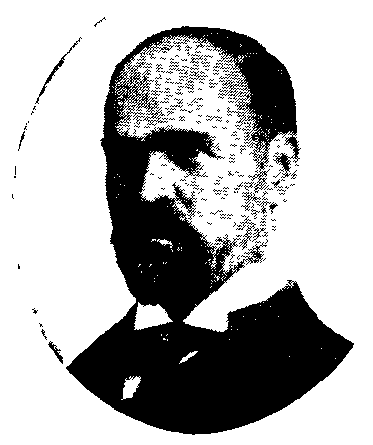
\includegraphics[width=25mm]{images/AMpic.png} \\
\textsc{Alexander Macfarlane}\\
From a photograph of 1898
\end{center}

\tableofcontents

%%PORTRAITS of MATHEMATICIANS

%% GEORGE PEACOCK (1791-1858)
%% A Lecture delivered April 12, 1901.

%% AUGUSTUS DE MORGAN (1806-1871)
%% A Lecture delivered April 13, 1901.

%% SIR WILLIAM ROWAN HAMILTON (1805-1865)
%% A Lecture delivered April 16, 1901.

%% GEORGE BOOLE (1815-1864)
%% A Lecture delivered April 19, 1901.

%% ARTHUR CAYLEY (1821-1895)
%% A Lecture delivered April 20, 1901.

%% WILLIAM KINGDON CLIFFORD (1845-1879)
%% A Lecture delivered April 23, 1901.

%% HENRY JOHN STEPHEN SMITH (1826-1883)
%% A Lecture delivered March 15, 1902.

%% JAMES JOSEPH SYLVESTER (1814-1897)
%% A Lecture delivered March 21, 1902.

%% THOMAS PENYNGTON KIRKMAN (1806-1895)
%% A Lecture delivered April 20, 1903.

%% ISAAC TODHUNTER (1820-1884)
%% A Lecture delivered April 13, 1904.

%% INDEX

\MainMatter

\chapter [George Peacock (1791-1858)]
{GEORGE PEACOCK\footnote{This Lecture was delivered April 12,
1901.---\textsc{Editors.}}}

\large\begin{center}{(1791-1858)}\end{center}\normalsize

George Peacock was born on April 9, 1791, at Denton in the north
of England, 14 miles from Richmond in Yorkshire. His father, the
Rev.\ Thomas Peacock, was a clergyman of the Church of England,
incumbent and for 50 years curate of the parish of Denton, where
he also kept a school. In early life Peacock did not show any
precocity of genius, and was more remarkable for daring feats of
climbing than for any special attachment to study. He received his
elementary education from his father, and at 17 years of age, was
sent to Richmond, to a school taught by a graduate of Cambridge
University to receive instruction preparatory to entering that
University. At this school he distinguished himself greatly both
in classics and in the rather elementary mathematics then required
for entrance at Cambridge. In 1809 he became a student of Trinity
College, Cambridge.

Here it may be well to give a brief account of that University, as
it was the alma mater of four out of the six mathematicians
discussed in this course of lectures\footnote{Dr.\ Macfarlane's
first course included the first six lectures given in this
volume.---\textsc{Editors.}}.

At that time the University of Cambridge consisted of seventeen
colleges, each of which had an independent endowment, buildings,
master, fellows and scholars. The endowments, generally in the
shape of lands, have come down from ancient times; for example,
Trinity College was founded by Henry VIII in 1546, and at the
beginning of the 19th century it consisted of a master, 60 fellows
and 72 scholars. Each college was provided with residence halls, a
dining hall, and a chapel. Each college had its own staff of
instructors called tutors or lecturers, and the function of the
University apart from the colleges was mainly to examine for
degrees. Examinations for degrees consisted of a pass examination
and an honors examination, the latter called a tripos. Thus, the
mathematical tripos meant the examinations of candidates for the
degree of Bachelor of Arts who had made a special study of
mathematics. The examination was spread over a week, and those who
obtained honors were divided into three classes, the highest class
being called \emph{wranglers}, and the highest man among the
wranglers, \emph{senior wrangler}. In more recent times this
examination developed into what De~Morgan called a ``great writing
race;'' the questions being of the nature of short problems. A
candidate put himself under the training of a coach, that is, a
mathematician who made it a business to study the kind of problems
likely to be set, and to train men to solve and write out the
solution of as many as possible per hour. As a consequence the
lectures of the University professors and the instruction of the
college tutors were neglected, and nothing was studied except what
would pay in the tripos examination. Modifications have been
introduced to counteract these evils, and the conditions have been
so changed that there are now no senior wranglers. The tripos
examination used to be followed almost immediately by another
examination in higher mathematics to determine the award of two
prizes named the Smith's prizes. ``Senior wrangler'' was
considered the greatest academic distinction in England.

In 1812 Peacock took the rank of second wrangler, and the second
Smith's prize, the senior wrangler being John Herschel. Two years
later he became a candidate for a fellowship in his college and
won it immediately, partly by means of his extensive and accurate
knowledge of the classics. A fellowship then meant about
\pounds200 a year, tenable for seven years provided the Fellow did
not marry meanwhile, and capable of being extended after the seven
years provided the Fellow took clerical Orders. The limitation to
seven years, although the Fellow devoted himself exclusively to
science, cut short and prevented by anticipation the career of
many a laborer for the advancement of science. Sir Isaac Newton
was a Fellow of Trinity College, and its limited terms nearly
deprived the world of the \emph{Principia}.

The year after taking a Fellowship, Peacock was appointed a tutor
and lecturer of his college, which position he continued to hold
for many years. At that time the state of mathematical learning at
Cambridge was discreditable. How could that be? you may ask; was
not Newton a professor of mathematics in that University? did he
not write the \emph{Principia} in Trinity College? had his
influence died out so soon? The true reason was he was worshipped
too much as an authority; the University had settled down to the
study of Newton instead of Nature, and they had followed him in
one grand mistake---the ignoring of the differential notation in
the calculus. Students of the differential calculus are more or
less familiar with the controversy which raged over the respective
claims of Newton and Leibnitz to the invention of the calculus;
rather over the question whether Leibnitz was an independent
inventor, or appropriated the fundamental ideas from Newton's
writings and correspondence, merely giving them a new clothing in
the form of the differential notation. Anyhow, Newton's countrymen
adopted the latter alternative; they clung to the fluxional
notation of Newton; and following Newton, they ignored the
notation of Leibnitz and everything written in that notation. The
Newtonian notation is as follows: If $y$ denotes a fluent, then
$\dot{y}$ denotes its fluxion, and $\ddot{y}$ the fluxion of
$\dot{y}$; if $y$ itself be considered a fluxion, then $y^\prime$
denotes its fluent, and $y^{\prime\prime}$ the fluent of
$y^\prime$ and so on; a differential is denoted by \textsc{o}. In
the notation of Leibnitz $\dot{y}$ is written $\frac{dy}{dx}$,
$\ddot{y}$ is written $\frac{d^2 y}{dx^2}$, $y^\prime$ is
$\int\!ydx$, and so on. The result of this Chauvinism on the part
of the British mathematicians of the eighteenth century was that
the developments of the calculus were made by the contemporary
mathematicians of the Continent, namely, the Bernoullis, Euler,
Clairault, Delambre, Lagrange, Laplace, Legendre. At the beginning
of the 19th century, there was only one mathematician in Great
Britain (namely Ivory, a Scotsman) who was familiar with the
achievements of the Continental mathematicians. Cambridge
University in particular was wholly given over not merely to the
use of the fluxional notation but to ignoring the differential
notation. The celebrated saying of Jacobi was then literally true,
although it had ceased to be true when he gave it utterance. He
visited Cambridge about 1842. When dining as a guest at the high
table of one of the colleges he was asked who in his opinion was
the greatest of the living mathematicians of England; his reply
was ``There is none.''

Peacock, in common with many other students of his own standing,
was profoundly impressed with the need of reform, and while still
an undergraduate formed a league with Babbage and Herschel to
adopt measures to bring it about. In 1815 they formed what they
called the \emph{Analytical Society}, the object of which was
stated to be to advocate the \emph{d}'ism of the Continent versus
the \emph{dot}-age of the University. Evidently the members of the
new society were armed with wit as well as mathematics. Of these
three reformers, Babbage afterwards became celebrated as the
inventor of an analytical engine, which could not only perform the
ordinary processes of arithmetic, but, when set with the proper
data, could tabulate the values of any function and print the
results. A part of the machine was constructed, but the inventor
and the Government (which was supplying the funds) quarrelled, in
consequence of which the complete machine exists only in the form
of drawings. These are now in the possession of the British
Government, and a scientific commission appointed to examine them
has reported that the engine could be constructed. The third
reformer---Herschel---was a son of Sir William Herschel, the
astronomer who discovered Uranus, and afterwards as Sir John
Herschel became famous as an astronomer and scientific
philosopher.

The first movement on the part of the Analytical Society was to
translate from the French the smaller work of Lacroix on the
differential and integral calculus; it was published in 1816. At
that time the best manuals, as well as the greatest works on
mathematics, existed in the French language. Peacock followed up
the translation with a volume containing a copious
\emph{Collection of Examples of the Application of the
Differential and Integral Calculus}, which was published in 1820.
The sale of both books was rapid, and contributed materially to
further the object of the Society. Then high wranglers of one year
became the examiners of the mathematical tripos three or four
years afterwards. Peacock was appointed an examiner in 1817, and
he did not fail to make use of the position as a powerful lever to
advance the cause of reform. In his questions set for the
examination the differential notation was for the first time
officially employed in Cambridge. The innovation did not escape
censure, but he wrote to a friend as follows: ``I assure you that
I shall never cease to exert myself to the utmost in the cause of
reform, and that I will never decline any office which may
increase my power to effect it. I am nearly certain of being
nominated to the office of Moderator in the year 1818-1819, and as
I am an examiner in virtue of my office, for the next year I shall
pursue a course even more decided than hitherto, since I shall
feel that men have been prepared for the change, and will then be
enabled to have acquired a better system by the publication of
improved elementary books. I have considerable influence as a
lecturer, and I will not neglect it. It is by silent perseverance
only, that we can hope to reduce the many-headed monster of
prejudice and make the University answer her character as the
loving mother of good learning and science.'' These few sentences
give an insight into the character of Peacock: he was an ardent
reformer and a few years brought success to the cause of the
Analytical Society.

Another reform at which Peacock labored was the teaching of
algebra. In 1830 he published a \emph{Treatise on Algebra} which
had for its object the placing of algebra on a true scientific
basis, adequate for the development which it had received at the
hands of the Continental mathematicians. As to the state of the
science of algebra in Great Britain, it may be judged of by the
following facts. Baron Maseres, a Fellow of Clare College,
Cambridge, and William Frend, a second wrangler, had both written
books protesting against the use of the negative quantity. Frend
published his \emph{Principles of Algebra} in 1796, and the
preface reads as follows: ``The ideas of number are the clearest
and most distinct of the human mind; the acts of the mind upon
them are equally simple and clear. There cannot be confusion in
them, unless numbers too great for the comprehension of the
learner are employed, or some arts are used which are not
justifiable. The first error in teaching the first principles of
algebra is obvious on perusing a few pages only of the first part
of Maclaurin's \emph{Algebra}. Numbers are there divided into two
sorts, positive and negative; and an attempt is made to explain
the nature of negative numbers by allusion to book debts and other
arts. Now when a person cannot explain the principles of a science
without reference to a metaphor, the probability is, that he has
never thought accurately upon the subject. A number may be greater
or less than another number; it may be added to, taken from,
multiplied into, or divided by, another number; but in other
respects it is very intractable; though the whole world should be
destroyed, one will be one, and three will be three, and no art
whatever can change their nature. You may put a mark before one,
which it will obey; it submits to be taken away from a number
greater than itself, but to attempt to take it away from a number
less than itself is ridiculous. Yet this is attempted by
algebraists who talk of a number less than nothing; of multiplying
a negative number into a negative number and thus producing a
positive number; of a number being imaginary. Hence they talk of
two roots to every equation of the second order, and the learner
is to try which will succeed in a given equation; they talk of
solving an equation which requires two impossible roots to make it
soluble; they can find out some impossible numbers which being
multiplied together produce unity. This is all jargon, at which
common sense recoils; but from its having been once adopted, like
many other figments, it finds the most strenuous supporters among
those who love to take things upon trust and hate the colour of a
serious thought.'' So far, Frend. Peacock knew that Argand,
Fran\c{c}ais and Warren had given what seemed to be an explanation
not only of the negative quantity but of the imaginary, and his
object was to reform the teaching of algebra so as to give it a
true scientific basis.

At that time every part of exact science was languishing in Great
Britain. Here is the description given by Sir John Herschel: ``The
end of the 18th and the beginning of the 19th century were
remarkable for the small amount of scientific movement going on in
Great Britain, especially in its more exact departments.
Mathematics were at the last gasp, and Astronomy nearly so---I
mean in those members of its frame which depend upon precise
measurement and systematic calculation. The chilling torpor of
routine had begun to spread itself over all those branches of
Science which wanted the excitement of experimental research.'' To
elevate astronomical science the Astronomical Society of London
was founded, and our three reformers Peacock, Babbage and Herschel
were prime movers in the undertaking. Peacock was one of the most
zealous promoters of an astronomical observatory at Cambridge, and
one of the founders of the Philosophical Society of Cambridge.

The year 1831 saw the beginning of one of the greatest scientific
organizations of modern times. That year the British Association
for the Advancement of Science (prototype of the American, French
and Australasian Associations) held its first meeting in the
ancient city of York. Its objects were stated to be: first, to
give a stronger impulse and a more systematic direction to
scientific enquiry; second, to promote the intercourse of those
who cultivate science in different parts of the British Empire
with one another and with foreign philosophers; third, to obtain a
more general attention to the objects of science, and the removal
of any disadvantages of a public kind which impede its progress.
One of the first resolutions adopted was to procure reports on the
state and progress of particular sciences, to be drawn up from
time to time by competent persons for the information of the
annual meetings, and the first to be placed on the list was a
report on the progress of mathematical science. Dr.\ Whewell, the
mathematician and philosopher, was a Vice-president of the
meeting: he was instructed to select the reporter. He first asked
Sir W.~R.\ Hamilton, who declined; he then asked Peacock, who
accepted. Peacock had his report ready for the third meeting of
the Association, which was held in Cambridge in 1833; although
limited to Algebra, Trigonometry, and the Arithmetic of Sines, it
is one of the best of the long series of valuable reports which
have been prepared for and printed by the Association.

In 1837 he was appointed Lowndean professor of astronomy in the
University of Cambridge, the chair afterwards occupied by Adams,
the co-discoverer of Neptune, and now occupied by Sir Robert Ball,
celebrated for his \emph{Theory of Screws}. In 1839 he was
appointed Dean of Ely, the diocese of Cambridge. While holding
this position he wrote a text book on algebra in two volumes, the
one called \emph{Arithmetical Algebra}, and the other
\emph{Symbolical Algebra}. Another object of reform was the
statutes of the University; he worked hard at it and was made a
member of a commission appointed by the Government for the
purpose; but he died on November 8, 1858, in the 68th year of his
age. His last public act was to attend a meeting of the
Commission.

Peacock's main contribution to mathematical analysis is his
attempt to place algebra on a strictly logical basis. He founded
what has been called the philological or symbolical school of
mathematicians; to which Gregory, De~Morgan and Boole belonged.
His answer to Maseres and Frend was that the science of algebra
consisted of two parts---arithmetical algebra and symbolical
algebra---and that they erred in restricting the science to the
arithmetical part. His view of arithmetical algebra is as follows:
``In arithmetical algebra we consider symbols as representing
numbers, and the operations to which they are submitted as
included in the same definitions as in common arithmetic; the
signs $+$ and $-$ denote the operations of addition and
subtraction in their ordinary meaning only, and those operations
are considered as impossible in all cases where the symbols
subjected to them possess values which would render them so in
case they were replaced by digital numbers; thus in expressions
such as $a + b$ we must suppose $a$ and $b$ to be quantities of
the same kind; in others, like $a - b$, we must suppose $a$
greater than $b$ and therefore homogeneous with it; in products
and quotients, like $ab$ and $\frac{a}{b}$ we must suppose the
multiplier and divisor to be abstract numbers; all results
whatsoever, including negative quantities, which are not strictly
deducible as legitimate conclusions from the definitions of the
several operations must be rejected as impossible, or as foreign
to the science.''

Peacock's principle may be stated thus: the elementary symbol of
arithmetical algebra denotes a digital, i.e., an integer number;
and every combination of elementary symbols must reduce to a
digital number, otherwise it is impossible or foreign to the
science. If $a$ and $b$ are numbers, then $a + b$ is always a
number; but $a - b$ is a number only when $b$ is less than $a$.
Again, under the same conditions, $ab$ is always a number, but
$\frac{a}{b}$ is really a number only when $b$ is an exact divisor
of $a$. Hence we are reduced to the following dilemma: Either
$\frac{a}{b}$ must be held to be an impossible expression in
general, or else the meaning of the fundamental symbol of algebra
must be extended so as to include rational fractions. If the
former horn of the dilemma is chosen, arithmetical algebra becomes
a mere shadow; if the latter horn is chosen, the operations of
algebra cannot be defined on the supposition that the elementary
symbol is an integer number. Peacock attempts to get out of the
difficulty by supposing that a symbol which is used as a
multiplier is always an integer number, but that a symbol in the
place of the multiplicand may be a fraction. For instance, in
$ab$, $a$ can denote only an integer number, but $b$ may denote a
rational fraction. Now there is no more fundamental principle in
arithmetical algebra than that $ab = ba$; which would be
illegitimate on Peacock's principle.

One of the earliest English writers on arithmetic is Robert
Record, who dedicated his work to King Edward the Sixth. The
author gives his treatise the form of a dialogue between master
and scholar. The scholar battles long over this difficulty,---that
multiplying a thing could make it less. The master attempts to
explain the anomaly by reference to proportion; that the product
due to a fraction bears the same proportion to the thing
multiplied that the fraction bears to unity. But the scholar is
not satisfied and the master goes on to say: ``If I multiply by
more than one, the thing is increased; if I take it but once, it
is not changed, and if I take it less than once, it cannot be so
much as it was before. Then seeing that a fraction is less than
one, if I multiply by a fraction, it follows that I do take it
less than once.'' Whereupon the scholar replies, ``Sir, I do thank
you much for this reason,---and I trust that I do perceive the
thing.''

The fact is that even in arithmetic the two processes of
multiplication and division are generalized into a common
multiplication; and the difficulty consists in passing from the
original idea of multiplication to the generalized idea of a
\emph{tensor}, which idea includes compressing the magnitude as
well as stretching it. Let $m$ denote an integer number; the next
step is to gain the idea of the reciprocal of $m$, not as
$\frac{1}{m}$ but simply as $/m$. When $m$ and $/n$ are compounded
we get the idea of a rational fraction; for in general $m/n$ will
not reduce to a number nor to the reciprocal of a number.

Suppose, however, that we pass over this objection; how does
Peacock lay the foundation for general algebra? He calls it
symbolical algebra, and he passes from arithmetical algebra to
symbolical algebra in the following manner: ``Symbolical algebra
adopts the rules of arithmetical algebra but removes altogether
their restrictions; thus symbolical subtraction differs from the
same operation in arithmetical algebra in being possible for all
relations of value of the symbols or expressions employed. All the
results of arithmetical algebra which are deduced by the
application of its rules, and which are general in form though
particular in value, are results likewise of symbolical algebra
where they are general in value as well as in form; thus the
product of $a^{m}$ and $a^{n}$ which is $a^{m+n}$ when $m$ and $n$
are whole numbers and therefore general in form though particular
in value, will be their product likewise when $m$ and $n$ are
general in value as well as in form; the series for $(a+b)^{n}$
determined by the principles of arithmetical algebra when $n$ is
any whole number, \emph{if it be exhibited in a general form,
without reference to a final term}, may be shown upon the same
principle to the equivalent series for $(a+b)^n$ when $n$ is
general both in form and value.''

The principle here indicated by means of examples was named by
Peacock the ``principle of the permanence of equivalent forms,''
and at page 59 of the \emph{Symbolical Algebra} it is thus
enunciated: ``Whatever algebraical forms are equivalent when the
symbols are general in form, but specific in value, will be
equivalent likewise when the symbols are general in value as well
as in form.''

For example, let $a$, $b$, $c$, $d$ denote any integer numbers,
but subject to the restrictions that $b$ is less than $a$, and $d$
less than $c$; it may then be shown arithmetically that
\begin{displaymath}
(a - b)(c - d)=ac + bd - ad - bc.
\end{displaymath}
Peacock's principle says that the form on the left side is
equivalent to the form on the right side, not only when the said
restrictions of being less are removed, but when $a$, $b$, $c$,
$d$ denote the most general algebraical symbol. It means that $a$,
$b$, $c$, $d$ may be rational fractions, or surds, or imaginary
quantities, or indeed operators such as $\frac{d}{dx}$. The
equivalence is not established by means of the nature of the
quantity denoted; the equivalence is assumed to be true, and then
it is attempted to find the different interpretations which may be
put on the symbol.

It is not difficult to see that the problem before us involves the
fundamental problem of a rational logic or theory of knowledge;
namely, how are we able to ascend from particular truths to more
general truths. If $a$, $b$, $c$, $d$ denote integer numbers, of
which $b$ is less than $a$ and $d$ less than $c$, then
\begin{displaymath}
(a - b)(c - d)=ac + bd - ad - bc.
\end{displaymath}
It is first seen that the above restrictions may be removed, and
still the above equation hold. But the antecedent is still too
narrow; the true scientific problem consists in specifying the
meaning of the symbols, which, and only which, will admit of the
forms being equal. It is not to find \emph{some meanings}, but the
\emph{most general meaning}, which allows the equivalence to be
true. Let us examine some other cases; we shall find that
Peacock's principle is not a solution of the difficulty; the great
logical process of generalization cannot be reduced to any such
easy and arbitrary procedure. When $a$, $m$, $n$ denote integer
numbers, it can be shown that
\begin{displaymath}
a^ma^n = a^{m+n}.
\end{displaymath}
According to Peacock the form on the left is always to be equal to
the form on the right, and the meanings of $a$, $m$, $n$ are to be
found by interpretation. Suppose that $a$ takes the form of the
incommensurate quantity $e$, the base of the natural system of
logarithms. A number is a degraded form of a complex quantity
$p+q^{\sqrt{-1}}$ and a complex quantity is a degraded form of a
quaternion; consequently one meaning which may be assigned to $m$
and $n$ is that of quaternion. Peacock's principle would lead us
to suppose that $e^me^n = e^{m+n}$, $m$ and $n$ denoting
quaternions; but that is just what Hamilton, the inventor of the
quaternion generalization, denies. There are reasons for believing
that he was mistaken, and that the forms remain equivalent even
under that extreme generalization of $m$ and $n$; but the point is
this: it is not a question of conventional definition and formal
truth; it is a question of objective definition and real truth.
Let the symbols have the prescribed meaning, does or does not the
equivalence still hold? And if it does not hold, what is the
higher or more complex form which the equivalence assumes?


\chapter [Augustus De~Morgan (1806-1871)]{AUGUSTUS
DE~MORGAN\footnote{This Lecture was delivered April 13,
1901.---\textsc{Editors.}}}

\large\begin{center}{(1806-1871)}\end{center}\normalsize

Augustus De~Morgan was born in the month of June at Madura in the
presidency of Madras, India; and the year of his birth may be
found by solving a conundrum proposed by himself, ``I was $x$
years of age in the year $x^2$.'' The problem is indeterminate,
but it is made strictly determinate by the century of its
utterance and the limit to a man's life. His father was Col.\
De~Morgan, who held various appointments in the service of the
East India Company. His mother was descended from James Dodson,
who computed a table of anti-logarithms, that is, the numbers
corresponding to exact logarithms. It was the time of the Sepoy
rebellion in India, and Col.\ De~Morgan removed his family to
England when Augustus was seven months old. As his father and
grandfather had both been born in India, De~Morgan used to say
that he was neither English, nor Scottish, nor Irish, but a Briton
``unattached,'' using the technical term applied to an
undergraduate of Oxford or Cambridge who is not a member of any
one of the Colleges.

When De~Morgan was ten years old, his father died. Mrs.\ De~Morgan
resided at various places in the southwest of England, and her son
received his elementary education at various schools of no great
account. His mathematical talents were unnoticed till he had
reached the age of fourteen. A friend of the family accidentally
discovered him making an elaborate drawing of a figure in Euclid
with ruler and compasses, and explained to him the aim of Euclid,
and gave him an initiation into demonstration.

De~Morgan suffered from a physical defect---one of his eyes was
rudimentary and useless. As a consequence, he did not join in the
sports of the other boys, and he was even made the victim of cruel
practical jokes by some schoolfellows. Some psychologists have
held that the perception of distance and of solidity depends on
the action of two eyes, but De~Morgan testified that so far as he
could make out he perceived with his one eye distance and solidity
just like other people.

He received his secondary education from Mr.\ Parsons, a Fellow of
Oriel College, Oxford, who could appreciate classics much better
than mathematics. His mother was an active and ardent member of
the Church of England, and desired that her son should become a
clergyman; but by this time De~Morgan had begun to show his
non-grooving disposition, due no doubt to some extent to his
physical infirmity. At the age of sixteen he was entered at
Trinity College, Cambridge, where he immediately came under the
tutorial influence of Peacock and Whewell. They became his
life-long friends; from the former he derived an interest in the
renovation of algebra, and from the latter an interest in the
renovation of logic---the two subjects of his future life work.

At college the flute, on which he played exquisitely, was his
recreation. He took no part in athletics but was prominent in the
musical clubs. His love of knowledge for its own sake interfered
with training for the great mathematical race; as a consequence he
came out fourth wrangler. This entitled him to the degree of
Bachelor of Arts; but to take the higher degree of Master of Arts
and thereby become eligible for a fellowship it was then necessary
to pass a theological test. To the signing of any such test
De~Morgan felt a strong objection, although he had been brought up
in the Church of England. About 1875 theological tests for
academic degrees were abolished in the Universities of Oxford and
Cambridge.

As no career was open to him at his own university, he decided to
go to the Bar, and took up residence in London; but he much
preferred teaching mathematics to reading law. About this time the
movement for founding the London University took shape. The two
ancient universities were so guarded by theological tests that no
Jew or Dissenter from the Church of England could enter as a
student; still less be appointed to any office. A body of
liberal-minded men resolved to meet the difficulty by establishing
in London a University on the principle of religious neutrality.
De~Morgan, then 22 years of age, was appointed Professor of
Mathematics. His introductory lecture ``On the study of
mathematics'' is a discourse upon mental education of permanent
value which has been recently reprinted in the United States.

The London University was a new institution, and the relations of
the Council of management, the Senate of professors and the body
of students were not well defined. A dispute arose between the
professor of anatomy and his students, and in consequence of the
action taken by the Council, several of the professors resigned,
headed by De~Morgan. Another professor of mathematics was
appointed, who was accidentally drowned a few years later.
De~Morgan had shown himself a prince of teachers: he was invited
to return to his chair, which thereafter became the continuous
center of his labors for thirty years.

The same body of reformers---headed by Lord Brougham, a Scotsman
eminent both in science and politics---who had instituted the
London University, founded about the same time a Society for the
Diffusion of Useful Knowledge. Its object was to spread scientific
and other knowledge by means of cheap and clearly written
treatises by the best writers of the time. One of its most
voluminous and effective writers was De~Morgan. He wrote a great
work on \emph{The Differential and Integral Calculus} which was
published by the Society; and he wrote one-sixth of the articles
in the \emph{Penny Cyclopedia}, published by the Society, and
issued in penny numbers. When De~Morgan came to reside in London
he found a congenial friend in William Frend, notwithstanding his
mathematical heresy about negative quantities. Both were
arithmeticians and actuaries, and their religious views were
somewhat similar. Frend lived in what was then a suburb of London,
in a country-house formerly occupied by Daniel Defoe and Isaac
Watts. De~Morgan with his flute was a welcome visitor; and in 1837
he married Sophia Elizabeth, one of Frend's daughters.

The London University of which De~Morgan was a professor was a
different institution from the University of London. The
University of London was founded about ten years later by the
Government for the purpose of granting degrees after examination,
without any qualification as to residence. The London University
was affiliated as a teaching college with the University of
London, and its name was changed to University College. The
University of London was not a success as an examining body; a
teaching University was demanded. De~Morgan was a highly
successful teacher of mathematics. It was his plan to lecture for
an hour, and at the close of each lecture to give out a number of
problems and examples illustrative of the subject lectured on; his
students were required to sit down to them and bring him the
results, which he looked over and returned revised before the next
lecture. In De~Morgan's opinion, a thorough comprehension and
mental assimilation of great principles far outweighed in
importance any merely analytical dexterity in the application of
half-understood principles to particular cases.

De~Morgan had a son George, who acquired great distinction in
mathematics both at University College and the University of
London. He and another like-minded alumnus conceived the idea of
founding a Mathematical Society in London, where mathematical
papers would be not only received (as by the Royal Society) but
actually read and discussed. The first meeting was held in
University College; De~Morgan was the first president, his son the
first secretary. It was the beginning of the London Mathematical
Society. In the year 1866 the chair of mental philosophy in
University College fell vacant. Dr.\ Martineau, a Unitarian
clergyman and professor of mental philosophy, was recommended
formally by the Senate to the Council; but in the Council there
were some who objected to a Unitarian clergyman, and others who
objected to theistic philosophy. A layman of the school of Bain
and Spencer was appointed. De~Morgan considered that the old
standard of religious neutrality had been hauled down, and
forthwith resigned. He was now 60 years of age. His pupils secured
a pension of \$500 for him, but misfortunes followed. Two years
later his son George---the younger Bernoulli, as he loved to hear
him called, in allusion to the two eminent mathematicians of that
name, related as father and son---died. This blow was followed by
the death of a daughter. Five years after his resignation from
University College De~Morgan died of nervous prostration on March
18, 1871, in the 65th year of his age.

De~Morgan was a brilliant and witty writer, whether as a
controversialist or as a correspondent. In his time there
flourished two Sir William Hamiltons who have often been
confounded. The one Sir William was a baronet (that is, inherited
the title), a Scotsman, professor of logic and metaphysics in the
University of Edinburgh; the other was a knight (that is, won the
title), an Irishman, professor of astronomy in the University of
Dublin. The baronet contributed to logic the doctrine of the
quantification of the predicate; the knight, whose full name was
William Rowan Hamilton, contributed to mathematics the geometric
algebra called Quaternions. De~Morgan was interested in the work
of both, and corresponded with both; but the correspondence with
the Scotsman ended in a public controversy, whereas that with the
Irishman was marked by friendship and terminated only by death. In
one of his letters to Rowan, De~Morgan says, ``Be it known unto
you that I have discovered that you and the other Sir W.~H.\ are
reciprocal polars with respect to me (intellectually and morally,
for the Scottish baronet is a polar bear, and you, I was going to
say, are a polar gentleman). When I send a bit of investigation to
Edinburgh, the W.~H.\ of that ilk says I took it from him. When I
send you one, you take it from me, generalize it at a glance,
bestow it thus generalized upon society at large, and make me the
second discoverer of a known theorem.''

The correspondence of De~Morgan with Hamilton the mathematician
extended over twenty-four years; it contains discussions not only
of mathematical matters, but also of subjects of general interest.
It is marked by geniality on the part of Hamilton and by wit on
the part of De~Morgan. The following is a specimen: Hamilton
wrote, ``My copy of Berkeley's work is not mine; like Berkeley,
you know, I am an Irishman.'' De~Morgan replied, ``Your phrase `my
copy is not mine' is not a bull. It is perfectly good English to
use the same word in two different senses in one sentence,
particularly when there is usage. Incongruity of language is no
bull, for it expresses meaning. But incongruity of ideas (as in
the case of the Irishman who was pulling up the rope, and finding
it did not finish, cried out that somebody had cut off the other
end of it) is the genuine bull.''

De~Morgan was full of personal peculiarities. We have noticed his
almost morbid attitude towards religion, and the readiness with
which he would resign an office. On the occasion of the
installation of his friend, Lord Brougham, as Rector of the
University of Edinburgh, the Senate offered to confer on him the
honorary degree of LL.D.; he declined the honor as a misnomer. He
once printed his name: Augustus De~Morgan,
\begin{displaymath}
\mbox{H}\cdot\mbox{O}\cdot\mbox{M}\cdot\mbox{O}\,\cdot\,
\mbox{P}\cdot\mbox{A}\cdot\mbox{U}\cdot\mbox{C}\cdot\mbox{A}
\cdot\mbox{R}\cdot\mbox{U}\cdot\mbox{M}\,\cdot\,\mbox{L}\cdot\mbox{I}
\cdot\mbox{T}\cdot\mbox{E}\cdot\mbox{R}\cdot\mbox{A}\cdot\mbox{R}
\cdot\mbox{U}\cdot\mbox{M.}
\end{displaymath}
\noindent He disliked the country, and while his family enjoyed
the seaside, and men of science were having a good time at a
meeting of the British Association in the country he remained in
the hot and dusty libraries of the metropolis. He said that he
felt like Socrates, who declared that the farther he got from
Athens the farther was he from happiness. He never sought to
become a Fellow of the Royal Society, and he never attended a
meeting of the Society; he said that he had no ideas or sympathies
in common with the physical philosopher. His attitude was
doubtless due to his physical infirmity, which prevented him from
being either an observer or an experimenter. He never voted at an
election, and he never visited the House of Commons, or the Tower,
or Westminster Abbey.

Were the writings of De~Morgan published in the form of collected
works, they would form a small library. We have noticed his
writings for the Useful Knowledge Society. Mainly through the
efforts of Peacock and Whewell, a Philosophical Society had been
inaugurated at Cambridge; and to its Transactions De~Morgan
contributed four memoirs on the foundations of algebra, and an
equal number on formal logic. The best presentation of his view of
algebra is found in a volume, entitled \emph{Trigonometry and
Double Algebra}, published in 1849; and his earlier view of formal
logic is found in a volume published in 1847. His most unique work
is styled a \emph{Budget of Paradoxes}; it originally appeared as
letters in the columns of the \emph{Athen\ae{}um} journal; it was
revised and extended by De~Morgan in the last years of his life,
and was published posthumously by his widow. ``If you wish to read
something entertaining,'' said Professor Tait to me, ``get
De~Morgan's \emph{Budget of Paradoxes} out of the library.'' We
shall consider more at length his theory of algebra, his
contribution to exact logic, and his Budget of Paradoxes.

In my last lecture I explained Peacock's theory of algebra. It was
much improved by D.~F.\ Gregory, a younger member of the Cambridge
School, who laid stress not on the permanence of equivalent forms,
but on the permanence of certain formal laws. This new theory of
algebra as the science of symbols and of their laws of combination
was carried to its logical issue by De~Morgan; and his doctrine on
the subject is still followed by English algebraists in general.
Thus Chrystal founds his \emph{Textbook of Algebra} on De~Morgan's
theory; although an attentive reader may remark that he
practically abandons it when he takes up the subject of infinite
series. De~Morgan's theory is stated in his volume on
\emph{Trigonometry and Double Algebra}. In the chapter (of the
book) headed ``On symbolic algebra'' he writes: ``In abandoning
the meaning of symbols, we also abandon those of the words which
describe them. Thus addition is to be, for the present, a sound
void of sense. It is a mode of combination represented by $+$;
when $+$ receives its meaning, so also will the word addition. It
is most important that the student should bear in mind that, with
one exception, no word nor sign of arithmetic or algebra has one
atom of meaning throughout this chapter, the object of which is
symbols, and their laws of combination, giving a symbolic algebra
which may hereafter become the grammar of a hundred distinct
significant algebras. If any one were to assert that $+$ and $-$
might mean reward and punishment, and $A$, $B$, $C$, etc., might
stand for virtues and vices, the reader might believe him, or
contradict him, as he pleases, but not out of this chapter. The
one exception above noted, which has some share of meaning, is the
sign $=$ placed between two symbols as in $A = B$. It indicates
that the two symbols have the same resulting meaning, by whatever
steps attained. That $A$ and $B$, if quantities, are the same
amount of quantity; that if operations, they are of the same
effect, etc.''

Here, it may be asked, why does the symbol $=$ prove refractory to
the symbolic theory? De~Morgan admits that there is one exception;
but an exception proves the rule, not in the usual but illogical
sense of establishing it, but in the old and logical sense of
testing its validity. If an exception can be established, the rule
must fall, or at least must be modified. Here I am talking not of
grammatical rules, but of the rules of science or nature.

De~Morgan proceeds to give an inventory of the fundamental symbols
of algebra, and also an inventory of the laws of algebra. The
symbols are $0$, $1$, $+$, $-$, $\times$, $\div$, $(\,)^{(\,)}$, and
letters; these only, all others are derived. His inventory of the
fundamental laws is expressed under fourteen heads, but some of
them are merely definitions. The laws proper may be reduced to the
following, which, as he admits, are not all independent of one
another:
\begin{enumerate}[I.]
\item Law of signs. $+ + = +$, $+ - = -$, $- + = -$, $- - = +$,
$\times \times = \times$, $\times \div = \div$, $\div \times =
\div$, $\div \div = \times$.
\item Commutative law. $a+b = b+a$, $ab=ba$.
\item Distributive law. $a(b+c) = ab+ac$.
\item Index laws. $a^b \times a^c = a^{b+c}$, $(a^b)^c = a^{bc}$,
$(ab)^c = a^c b^c$.
\item $a- a= 0$, $a \div a = 1$.
\end{enumerate}
\noindent The last two may be called the rules of reduction.
De~Morgan professes to give a complete inventory of the laws which
the symbols of algebra must obey, for he says, ``Any system of
symbols which obeys these laws and no others, except they be
formed by combination of these laws, and which uses the preceding
symbols and no others, except they be new symbols invented in
abbreviation of combinations of these symbols, is symbolic
algebra.'' From his point of view, none of the above principles
are rules; they are formal laws, that is, arbitrarily chosen
relations to which the algebraic symbols must be subject. He does
not mention the law, which had already been pointed out by
Gregory, namely, $(a+b)+c = a+(b+c), (ab)c = a(bc)$ and to which
was afterwards given the name of the \emph{law of association}. If
the commutative law fails, the associative may hold good; but not
\emph{vice versa}. It is an unfortunate thing for the symbolist or
formalist that in universal arithmetic $m^n$ is not equal to
$n^m$; for then the commutative law would have full scope. Why
does he not give it full scope? Because the foundations of algebra
are, after all, real not formal, material not symbolic. To the
formalists the index operations are exceedingly refractory, in
consequence of which some take no account of them, but relegate
them to applied mathematics. To give an inventory of the laws
which the symbols of algebra must obey is an impossible task, and
reminds one not a little of the task of those philosophers who
attempt to give an inventory of the \emph{a priori} knowledge of
the mind.

De~Morgan's work entitled \emph{Trigonometry and Double Algebra}
consists of two parts; the former of which is a treatise on
Trigonometry, and the latter a treatise on generalized algebra
which he calls Double Algebra. But what is meant by Double as
applied to algebra? and why should Trigonometry be also treated in
the same textbook? The first stage in the development of algebra
is \emph{arithmetic}, where numbers only appear and symbols of
operations such as $+$, $\times$, etc. The next stage is
\emph{universal arithmetic}, where letters appear instead of
numbers, so as to denote numbers universally, and the processes
are conducted without knowing the values of the symbols. Let $a$
and $b$ denote any numbers; then such an expression as $a-b$ may
be impossible; so that in universal arithmetic there is always a
proviso, \emph{provided the operation is possible}. The third
stage is \emph{single algebra}, where the symbol may denote a
quantity forwards or a quantity backwards, and is adequately
represented by segments on a straight line passing through an
origin. Negative quantities are then no longer impossible; they
are represented by the backward segment. But an impossibility
still remains in the latter part of such an expression as
$a+b\sqrt{-1}$ which arises in the solution of the quadratic
equation. The fourth stage is \emph{double algebra}; the algebraic
symbol denotes in general a segment of a line in a given plane; it
is a double symbol because it involves two specifications, namely,
length and direction; and $\sqrt{-1}$ is interpreted as denoting a
quadrant. The expression $a+b\sqrt{-1}$ then represents a line in
the plane having an abscissa $a$ and an ordinate $b$. Argand and
Warren carried double algebra so far; but they were unable to
interpret on this theory such an expression as $e^{a\sqrt{-1}}$.
De~Morgan attempted it by \emph{reducing} such an expression to
the form $b+q\sqrt{-1}$, and he considered that he had shown that
it could be always so reduced. The remarkable fact is that this
double algebra satisfies all the fundamental laws above
enumerated, and as every apparently impossible combination of
symbols has been interpreted it looks like the complete form of
algebra.

If the above theory is true, the next stage of development ought
to be \emph{triple} algebra and if $a+b\sqrt{-1}$ truly represents
a line in a given plane, it ought to be possible to find a third
term which added to the above would represent a line in space.
Argand and some others guessed that it was $a + b\sqrt{-1} +
c\sqrt{-1}\,^{\sqrt{-1}}$ although this contradicts the truth
established by Euler that $\sqrt{-1}\,^{\sqrt{-1}}=e^{-
\frac{1}{2} \pi}$. De~Morgan and many others worked hard at the
problem, but nothing came of it until the problem was taken up by
Hamilton. We now see the reason clearly: the symbol of double
algebra denotes not a length and a direction; but a multiplier and
\emph{an angle}. In it the angles are confined to one plane; hence
the next stage will be a \emph{quadruple algebra}, when the axis
of the plane is made variable. And this gives the answer to the
first question; double algebra is nothing but analytical plane
trigonometry, and this is the reason why it has been found to be
the natural analysis for alternating currents. But De~Morgan never
got this far; he died with the belief ``that double algebra must
remain as the full development of the conceptions of arithmetic,
so far as those symbols are concerned which arithmetic immediately
suggests.''

When the study of mathematics revived at the University of
Cambridge, so also did the study of logic. The moving spirit was
Whewell, the Master of Trinity College, whose principal writings
were a \emph{History of the Inductive Sciences}, and
\emph{Philosophy of the Inductive Sciences}. Doubtless De~Morgan
was influenced in his logical investigations by Whewell; but other
contemporaries of influence were Sir W.\ Hamilton of Edinburgh, and
Professor Boole of Cork. De~Morgan's work on \emph{Formal Logic},
published in 1847, is principally remarkable for his development
of the numerically definite syllogism. The followers of Aristotle
say and say truly that from two particular propositions such as
\emph{Some} $M$'s \emph{are} $A$'s, and \emph{Some} $M$'s
\emph{are} $B$'s nothing follows of necessity about the relation
of the $A$'s and $B$'s. But they go further and say in order that
any relation about the $A$'s and $B$'s may follow of necessity,
the middle term must be taken universally in one of the premises.
De~Morgan pointed out that from \emph{Most} $M$'s \emph{are} $A$'s
and \emph{Most} $M$'s \emph{are} $B$'s it follows of necessity
that some $A$'s are $B$'s and he formulated the numerically
definite syllogism which puts this principle in exact quantitative
form. Suppose that the number of the $M$'s is $m$, of the $M$'s
that are $A$'s is $a$, and of the $M$'s that are $B$'s is $b$;
then there are at least $(a+b-m)$ $A$'s that are $B$'s. Suppose
that the number of souls on board a steamer was $1000$, that $500$
were in the saloon, and $700$ were lost; it follows of necessity,
that at least $700+500-1000$, that is, $200$, saloon passengers
were lost. This single principle suffices to prove the validity of
all the Aristotelian moods; it is therefore a fundamental
principle in necessary reasoning.

Here then De~Morgan had made a great advance by introducing
\emph{quantification of the terms}. At that time Sir W.\ Hamilton
was teaching at Edinburgh a doctrine of the quantification of the
predicate, and a correspondence sprang up. However, De~Morgan soon
perceived that Hamilton's quantification was of a different
character; that it meant for example, substituting the two forms
\emph{The whole of} $A$ \emph{is the whole of} $B$, and \emph{The
whole of} $A$ \emph{is a part of} $B$ for the Aristotelian form
All $A$'s are $B$'s. Philosophers generally have a large share of
intolerance; they are too apt to think that they have got hold of
the whole truth, and that everything outside of their system is
error. Hamilton thought that he had placed the keystone in the
Aristotelian arch, as he phrased it; although it must have been a
curious arch which could stand 2000 years without a keystone. As a
consequence he had no room for De~Morgan's innovations. He accused
De~Morgan of plagiarism, and the controversy raged for years in
the columns of the \emph{Athen\ae{}um}, and in the publications of
the two writers.

The memoirs on logic which De~Morgan contributed to the
Transactions of the Cambridge Philosophical Society subsequent to
the publication of his book on \emph{Formal Logic} are by far the
most important contributions which he made to the science,
especially his fourth memoir, in which he begins work in the broad
field of the \emph{logic of relatives}. This is the true field for
the logician of the twentieth century, in which work of the
greatest importance is to be done towards improving language and
facilitating thinking processes which occur all the time in
practical life. Identity and difference are the two relations
which have been considered by the logician; but there are many
others equally deserving of study, such as equality, equivalence,
consanguinity, affinity, etc.

In the introduction to the \emph{Budget of Paradoxes} De~Morgan
explains what he means by the word. ``A great many individuals,
ever since the rise of the mathematical method, have, each for
himself, attacked its direct and indirect consequences. I shall
call each of these persons a \emph{paradoxer}, and his system a
\emph{paradox}. I use the word in the old sense: a paradox is
something which is apart from general opinion, either in subject
matter, method, or conclusion. Many of the things brought forward
would now be called \emph{crotchets}, which is the nearest word we
have to old \emph{paradox}. But there is this difference, that by
calling a thing a crotchet we mean to speak lightly of it; which
was not the necessary sense of paradox. Thus in the 16th century
many spoke of the earth's motion as the \emph{paradox of
Copernicus} and held the ingenuity of that theory in very high
esteem, and some I think who even inclined towards it. In the
seventeenth century the depravation of meaning took place, in
England at least.''

How can the sound paradoxer be distinguished from the false
paradoxer? De~Morgan supplies the following test: ``The manner in
which a paradoxer will show himself, as to sense or nonsense, will
not depend upon what he maintains, but upon whether he has or has
not made a sufficient knowledge of what has been done by others,
especially as to the mode of doing it, a preliminary to inventing
knowledge for himself\ldots. New knowledge, when to any purpose,
must come by contemplation of old knowledge, in every matter which
concerns thought; mechanical contrivance sometimes, not very
often, escapes this rule. All the men who are now called
discoverers, in every matter ruled by thought, have been men
versed in the minds of their predecessors and learned in what had
been before them. There is not one exception.''

I remember that just before the American Association met at
Indianapolis in 1890, the local newspapers heralded a great
discovery which was to be laid before the assembled savants---a
young man living somewhere in the country had squared the circle.
While the meeting was in progress I observed a young man going
about with a roll of paper in his hand. He spoke to me and
complained that the paper containing his discovery had not been
received. I asked him whether his object in presenting the paper
was not to get it read, printed and published so that everyone
might inform himself of the result; to all of which he assented
readily. But, said I, many men have worked at this question, and
their results have been tested fully, and they are printed for the
benefit of anyone who can read; have you informed yourself of
their results? To this there was no assent, but the sickly smile
of the false paradoxer.

The \emph{Budget} consists of a review of a large collection of
paradoxical books which De~Morgan had accumulated in his own
library, partly by purchase at bookstands, partly from books sent
to him for review, partly from books sent to him by the authors.
He gives the following classification: squarers of the circle,
trisectors of the angle, duplicators of the cube, constructors of
perpetual motion, subverters of gravitation, stagnators of the
earth, builders of the universe. You will still find specimens of
all these classes in the New World and in the new century.

De~Morgan gives his personal knowledge of paradoxers. ``I suspect
that I know more of the English class than any man in Britain. I
never kept any reckoning: but I know that one year with
another?---and less of late years than in earlier time?---I have
talked to more than five in each year, giving more than a hundred
and fifty specimens. Of this I am sure, that it is my own fault if
they have not been a thousand. Nobody knows how they swarm, except
those to whom they naturally resort. They are in all ranks and
occupations, of all ages and characters. They are very earnest
people, and their purpose is bona fide, the dissemination of their
paradoxes. A great many---the mass, indeed---are illiterate, and a
great many waste their means, and are in or approaching penury.
These discoverers despise one another.''

A paradoxer to whom De~Morgan paid the compliment which Achilles
paid Hector---to drag him round the walls again and again---was
James Smith, a successful merchant of Liverpool. He found $\pi = 3
\frac{1}{8}$. His mode of reasoning was a curious caricature of
the \emph{reductio ad absurdum} of Euclid. He said let $\pi = 3
\frac{1}{8}$, and then showed that on that supposition, every
other value of $\pi$ must be absurd; consequently $\pi =
3\frac{1}{8}$ is the true value. The following is a specimen of De
Morgan's dragging round the walls of Troy: ``Mr.\ Smith continues
to write me long letters, to which he hints that I am to answer.
In his last of 31 closely written sides of note paper, he informs
me, with reference to my obstinate silence, that though I think
myself and am thought by others to be a mathematical Goliath, I
have resolved to play the mathematical snail, and keep within my
shell. A mathematical \emph{snail}! This cannot be the thing so
called which regulates the striking of a clock; for it would mean
that I am to make Mr.\ Smith sound the true time of day, which I
would by no means undertake upon a clock that gains 19 seconds odd
in every hour by false quadrative value of $\pi$. But he ventures
to tell me that pebbles from the sling of simple truth and common
sense will ultimately crack my shell, and put me \emph{hors de
combat}. The confusion of images is amusing: Goliath turning
himself into a snail to avoid $\pi = 3\frac{1}{8}$ and James
Smith, Esq., of the Mersey Dock Board: and put \emph{hors de
combat} by pebbles from a sling. If Goliath had crept into a snail
shell, David would have cracked the Philistine with his foot.
There is something like modesty in the implication that the
crack-shell pebble has not yet taken effect; it might have been
thought that the slinger would by this time have been
singing---And thrice [and one-eighth] I routed all my foes, And
thrice [and one-eighth] I slew the slain.''

In the region of pure mathematics De~Morgan could detect easily
the false from the true paradox; but he was not so proficient in
the field of physics. His father-in-law was a paradoxer, and his
wife a paradoxer; and in the opinion of the physical philosophers
De~Morgan himself scarcely escaped. His wife wrote a book
describing the phenomena of spiritualism, table-rapping,
table-turning, etc.; and De~Morgan wrote a preface in which he
said that he knew some of the asserted facts, believed others on
testimony, but did not pretend to know \emph{whether} they were
caused by spirits, or had some unknown and unimagined origin. From
this alternative he left out ordinary material causes. Faraday
delivered a lecture on \emph{Spiritualism}, in which he laid it
down that in the investigation we ought to set out with the idea
of what is physically possible, or impossible; De~Morgan could not
understand this.

\chapter [Sir William Rowan Hamilton (1805-1865)]{SIR WILLIAM
ROWAN~HAMILTON\footnote{This Lecture was delivered April 16,
1901.---\textsc{Editors.}}}

\large\begin{center}{(1805-1865)}\end{center}\normalsize

William Rowan Hamilton was born in Dublin, Ireland, on the 3d of
August, 1805. His father, Archibald Hamilton, was a solicitor in
the city of Dublin; his mother, Sarah Hutton, belonged to an
intellectual family, but she did not live to exercise much
influence on the education of her son. There has been some dispute
as to how far Ireland can claim Hamilton; Professor Tait of
Edinburgh in the Encyclopaedia Brittanica claims him as a
Scotsman, while his biographer, the Rev.\ Charles Graves, claims
him as essentially Irish. The facts appear to be as follows: His
father's mother was a Scotch woman; his father's father was a
citizen of Dublin. But the name ``Hamilton'' points to Scottish
origin, and Hamilton himself said that his family claimed to have
come over from Scotland in the time of James I\@. Hamilton always
considered himself an Irishman; and as Burns very early had an
ambition to achieve something for the renown of Scotland, so
Hamilton in his early years had a powerful ambition to do
something for the renown of Ireland. In later life he used to say
that at the beginning of the century people read French
mathematics, but that at the end of it they would be reading Irish
mathematics.

Hamilton, when three years of age, was placed in the charge of his
uncle, the Rev.\ James Hamilton, who was the curate of Trim, a
country town, about twenty miles from Dublin, and who was also the
master of the Church of England school. From his uncle he received
all his primary and secondary education and also instruction in
Oriental languages. As a child Hamilton was a prodigy; at three
years of age he was a superior reader of English and considerably
advanced in arithmetic; at four a good geographer; at five able to
read and translate Latin, Greek, and Hebrew, and liked to recite
Dryden, Collins, Milton and Homer; at eight a reader of Italian
and French and giving vent to his feelings in extemporized Latin;
at ten a student of Arabic and Sanscrit. When twelve years old he
met Zerah Colburn, the American calculating boy, and engaged with
him in trials of arithmetical skill, in which trials Hamilton came
off with honor, although Colburn was generally the victor. These
encounters gave Hamilton a decided taste for arithmetical
computation, and for many years afterwards he loved to perform
long operations in arithmetic in his mind, extracting the square
and cube root, and solving problems that related to the properties
of numbers. When thirteen he received his initiation into algebra
from Clairault's \emph{Algebra} in the French, and he made an
epitome, which he ambitiously entitled ``A Compendious Treatise on
Algebra by William Hamilton.''

When Hamilton was fourteen years old, his father died and left his
children slenderly provided for. Henceforth, as the elder brother
of three sisters, Hamilton had to act as a man. This year he
addressed a letter of welcome, written in the Persian language, to
the Persian Ambassador, then on a visit to Dublin; and he met
again Zerah Colburn. In the interval Zerah had attended one of the
great public schools of England. Hamilton had been at a country
school in Ireland, and was now able to make a successful
investigation of the methods by which Zerah made his lightning
calculations. When sixteen, Hamilton studied the Differential
Calculus by the help of a French textbook, and began the study of
the \emph{M\'ecanique c\'eleste} of Laplace, and he was able at
the beginning of this study to detect a flaw in the reasoning by
which Laplace demonstrates the theorem of the parallelogram of
forces. This criticism brought him to the notice of Dr.\ Brinkley,
who was then the professor of astronomy in the University of
Dublin, and resided at Dunkirk, about five miles from the centre
of the city. He also began an investigation for himself of
equations which represent systems of straight lines in a plane,
and in so doing hit upon ideas which he afterwards developed into
his first mathematical memoir to the Royal Irish Academy. Dr.\
Brinkley is said to have remarked of him at this time: ``This
young man, I do not say \emph{will be}, but \emph{is}, the first
mathematician of his age.''

At the age of eighteen Hamilton entered Trinity College, Dublin,
the University of Dublin founded by Queen Elizabeth, and differing
from the Universities of Oxford and Cambridge in having only one
college. Unlike Oxford, which has always given prominence to
classics, and Cambridge, which has always given prominence to
mathematics, Dublin at that time gave equal prominence to classics
and to mathematics. In his first year Hamilton won the very rare
honor of \emph{optime} at his examination in Homer. In the old
Universities marks used to be and in some cases still are
published, descending not in percentages but by means of the scale
of Latin adjectives: \emph{optime, valdebene, bene, satis,
mediocriter, vix medi, non}; \emph{optime} means passed with the
very highest distinction; \emph{vix} means passed but with great
difficulty. This scale is still in use in the medical examinations
of the University of Edinburgh. Before entering college Hamilton
had been accustomed to translate Homer into blank verse, comparing
his result with the translations of Pope and Cowper; and he had
already produced some original poems. In this, his first year he
wrote a poem ``On college ambition'' which is a fair specimen of
his poetical attainments.

\begin{verse}
  Oh! Ambition hath its hour \\
  Of deep and spirit-stirring power; \\
  Not in the tented field alone, \\
  Nor peer-engirded court and throne; \\
  Nor the intrigues of busy life; \\
  But ardent Boyhood's generous strife, \\
  While yet the Enthusiast spirit turns \\
  Where'er the light of Glory burns, \\
  Thinks not how transient is the blaze, \\
  But longs to barter Life for Praise.

  Look round the arena, and ye spy \\
  Pallid cheek and faded eye; \\
  Among the bands of rivals, few \\
  Keep their native healthy hue: \\
  Night and thought have stolen away \\
  Their once elastic spirit's play. \\
  A few short hours and all is o'er, \\
  Some shall win one triumph more; \\
  Some from the place of contest go \\
  Again defeated, sad and slow.

  What shall reward the conqueror then \\
  For all his toil, for all his pain, \\
  For every midnight throb that stole \\
  So often o'er his fevered soul? \\
  Is it the applaudings loud \\
  Or wond'ring gazes of the crowd; \\
  Disappointed envy's shame, \\
  Or hollow voice of fickle Fame? \\
  These may extort the sudden smile, \\
  May swell the heart a little while; \\
  But they leave no joy behind, \\
  Breathe no pure transport o'er the mind, \\
  Nor will the thought of selfish gladness \\
  Expand the brow of secret sadness.

  Yet if Ambition hath its hour \\
  Of deep and spirit-stirring power, \\
  Some bright rewards are all its own, \\
  And bless its votaries alone: \\
  The anxious friend's approving eye; \\
  The generous rivals' sympathy; \\
  And that best and sweetest prize \\
  Given by silent Beauty's eyes! \\
  These are transports true and strong, \\
  Deeply felt, remembered long: \\
  Time and sorrow passing o'er \\
  Endear their memory but the more.
\end{verse}

The ``silent Beauty'' was not an abstraction, but a young lady
whose brothers were fellow-students of Trinity College. This led
to much effusion of poetry; but unfortunately while Hamilton was
writing poetry about her another young man was talking prose to
her; with the result that Hamilton experienced a disappointment.
On account of his self-consciousness, inseparable probably from
his genius, he felt the disappointment keenly. He was then known
to the professor of astronomy, and walking from the College to the
Observatory along the Royal Canal, he was actually tempted to
terminate his life in the water.

In his second year he formed the plan of reading so as to compete
for the highest honors both in classics and in mathematics. At
graduation two gold medals were awarded, the one for distinction
in classics, the other for distinction in mathematics. Hamilton
aimed at carrying off both. In his junior year he received an
\emph{optime} in mathematical physics; and, as the winner of two
\emph{optimes}, the one in classics, the other in mathematics, he
immediately became a celebrity in the intellectual circle of
Dublin.

In his senior year he presented to the Royal Irish Academy a
memoir embodying his research on systems of lines. He now called
it a ``Theory of Systems of Rays'' and it was printed in the
\emph{Transactions}. About this time Dr.\ Brinkley was appointed
to the bishopric of Cloyne, and in consequence resigned the
professorship of astronomy. In the United Kingdom it is customary
when a post becomes vacant for aspirants to lodge a formal
application with the appointing board and to supplement their own
application by testimonial letters from competent authorities. In
the present case quite a number of candidates appeared, among them
Airy, who afterwards became Astronomer Royal of England, and
several Fellows of Trinity College, Dublin. Hamilton did not
become a formal candidate, but he was invited to apply, with the
result that he received the appointment while still an
undergraduate, and not twenty-two years of age. Thus was his
undergraduate career signalized much more than by the carrying off
of the two gold medals. Before assuming the duties of his chair he
made a tour through England and Scotland, and met for the first
time the poet Wordsworth at his home at Rydal Mount, in
Cumberland. They had a midnight walk, oscillating backwards and
forwards between Rydal and Ambleside, absorbed in converse on high
themes, and finding it almost impossible to part. Wordsworth
afterwards said that Coleridge and Hamilton were the two most
wonderful men, taking all their endowments together, that he had
ever met.

In October, 1827, he came to reside at the place which was
destined to be the scene of his scientific labors. I had the
pleasure of visiting it last summer as the guest of his successor.
The Observatory is situated on the top of a hill, Dunsink, about
five miles from Dublin. The house adjoins the observatory; to the
east is an extensive lawn; to the west a garden with stone wall
and shaded walks; to the south a terraced field; at the foot of
the hill is the Royal Canal; to the southeast the city of Dublin;
while the view is bounded by the sea and the Dublin and Wicklow
Mountains; a fine home for a poet or a philosopher or a
mathematician, and in Hamilton all three were combined.

Settled at the Observatory he started out diligently as an
observer, but he found it difficult to stand the low temperatures
incident to the work. He never attained skill as an observer, and
unfortunately he depended on a very poor assistant. Himself a
brilliant computer, with a good observer for assistant, the work
of the observatory ought to have flourished. One of the first
distinguished visitors at the Observatory was the poet Wordsworth,
in commemoration of which one of the shaded walks in the garden
was named Wordsworth's walk. Wordsworth advised him to concentrate
his powers on science; and, not long after, wrote him as follows:
``You send me showers of verses which I receive with much
pleasure, as do we all: yet have we fears that this employment may
seduce you from the path of science which you seem destined to
tread with so much honor to yourself and profit to others. Again
and again I must repeat that the composition of verse is
infinitely more of an art than men are prepared to believe, and
absolute success in it depends upon innumerable \emph{minuti\ae{}}
which it grieves me you should stoop to acquire a knowledge
of\ldots Again I do venture to submit to your consideration,
whether the poetical parts of your nature would not find a field
more favorable to their exercise in the regions of prose; not
because those regions are humbler, but because they may be
gracefully and profitably trod, with footsteps less careful and in
measures less elaborate.''

Hamilton possessed the poetic imagination; what he was deficient
in was the technique of the poet. The imagination of the poet is
kin to the imagination of the mathematician; both extract the
ideal from a mass of circumstances. In this connection De~Morgan
wrote: ``The moving power of mathetical \emph{invention} is not
reasoning but imagination. We no longer apply the homely term
\emph{maker} in literal translation of \emph{poet}; but
discoverers of all kinds, whatever may be their lines, are makers,
or, as we mow say, have the creative genius.'' Hamilton spoke of
the \emph{M\'ecanique analytique} of Lagrange as a ``scientific
poem''; Hamilton himself was styled the Irish Lagrange. Engineers
venerate Rankine, electricians venerate Maxwell; both were
scientific discoverers and likewise poets, that is, amateur poets.
The proximate cause of the shower of verses was that Hamilton had
fallen in love for the second time. The young lady was Miss
de~Vere, daughter of an accomplished Irish baronet, and who like
Tennyson's Lady Clara Vere de~Vere could look back on a long and
illustrious descent. Hamilton had a pupil in Lord Adare, the
eldest son of the Earl of Dunraven, and it was while visiting
Adare Manor that he was introduced to the De~Vere family, who
lived near by at Curragh Chase. His suit was encouraged by the
Countess of Dunraven, it was favorably received by both father and
mother, he had written many sonnets of which Ellen de~Vere was the
inspiration, he had discussed with her astronomy, poetry and
philosophy; and was on the eve of proposing when he gave up
because the young lady incidentally said to him that ``she could
not live happily anywhere but at Curragh.'' His action shows the
working of a too self-conscious mind, proud of his own
intellectual achievements, and too much awed by her long descent.
So he failed for the second time; but both of these ladies were
friends of his to the last.

At the age of 27 he contributed to the Irish Academy a
supplementary paper on his Theory of Systems of Rays, in which he
predicted the phenomenon of conical refraction; namely, that under
certain conditions a single ray incident on a biaxial crystal
would be broken up into a cone of rays, and likewise that under
certain conditions a single emergent ray would appear as a cone of
rays. The prediction was made by Hamilton on Oct.\ 22nd; it was
experimentally verified by his colleague Prof.\ Lloyd on Dec.\
14th. It is not experiment alone or mathematical reasoning alone
which has built up the splendid temple of physical science, but
the two working together; and of this we have a notable
exemplification in the discovery of conical refraction.

Twice Hamilton chose well but failed; now he made another choice
and succeeded. The lady was a Miss Bayly, who visited at the home
of her sister near Dunsink hill. The lady had serious misgivings
about the state of her health; but the marriage took place. The
kind of wife which Hamilton needed was one who could govern him
and efficiently supervise all domestic matters; but the wife he
chose was, from weakness of body and mind, incapable of doing it.
As a consequence, Hamilton worked for the rest of his life under
domestic difficulties of no ordinary kind.

At the age of 28 he made a notable addition to the theory of
Dynamics by extending to it the idea of a Characteristic Function,
which he had previously applied with success to the science of
Optics in his Theory of Systems of Rays. It was contributed to the
Royal Society of London, and printed in their \emph{Philosophical
Transactions}. The Royal Society of London is the great scientific
society of England, founded in the reign of Charles II, and of
which Newton was one of the early presidents; Hamilton was invited
to become a fellow but did not accept, as he could not afford the
expense.

At the age of 29 he read a paper before the Royal Irish Academy,
which set forth the result of long meditation and investigation on
the nature of Algebra as a science; the paper is entitled
``Algebra as the Science of Pure Time.'' The main idea is that as
Geometry considered as a science is founded upon the pure
intuition of space, so algebra as a science is founded upon the
pure intuition of time. He was never satisfied with Peacock's
theory of algebra as a ``System of Signs and their Combinations'';
nor with De~Morgan's improvement of it; he demanded a more real
foundation. In reading Kant's \emph{Critique of Pure Reason} he
was struck by the following passage: ``Time and space are two
sources of knowledge from which various \emph{a priori}
synthetical cognitions can be derived. Of this, pure mathematics
gives a splendid example in the case of our cognitions of space
and its various relations. As they are both pure forms of sensuous
intuition, they render synthetical propositions \emph{a priori}
possible.'' Thus, according to Kant, space and time are forms of
the intellect; and Hamilton reasoned that, as geometry is the
science of the former, so algebra must be the science of the
latter. When algebra is based on any unidimensional subject, such
as time, or a straight line, a difficulty arises in explaining the
roots of a quadratic equation when they are imaginary. To get over
this difficulty Hamilton invented a theory of algebraic couplets,
which has proved a conundrum in the mathematical world. Some 20
years ago there nourished in Edinburgh a mathematician named Sang
who had computed the most elaborate tables of logarithms in
existence---which still exist in manuscript. On reading the theory
in question he first judged that either Hamilton was crazy, or
else that he (Sang) was crazy, but eventually reached the more
comforting alternative. On the other hand, Prof.\ Tait believes in
its soundness, and endeavors to bring it down to the ordinary
comprehension.

We have seen that the British Association for the Advancement of
Science was founded in 1831, and that its first meeting was in the
ancient city of York. It was a policy of the founders not to meet
in London, but in the provincial cities, so that thereby greater
interest in the advance of science might be produced over the
whole land. The cities chosen for the place of meeting in
following years were the University towns: Oxford, Cambridge,
Edinburgh, Dublin. Hamilton was the only representative of Ireland
present at the Oxford meeting; and at the Oxford, Cambridge, and
Edinburgh meetings he not only contributed scientific papers, but
he acquired renown as a scientific orator. In the case of the
Dublin meeting he was chief organizer beforehand, and chief orator
when it met. The week of science was closed by a grand dinner
given in the library of Trinity College; and an incident took
place which is thus described by an American scientist:

``We assembled in the imposing hall of Trinity Library, two
hundred and eighty feet long, at six o'clock. When the company was
principally assembled, I observed a little stir near the place
where I stood, which nobody could explain, and which, in fact, was
not comprehended by more than two or three persons present. In a
moment, however, I perceived myself standing near the Lord
Lieutenant and his suite, in front of whom a space had been
cleared, and by whom was Professor Hamilton, looking very much
embarrassed. The Lord Lieutenant then called him by name, and he
stepped into the vacant space. `I am,' said his Excellency, `about
to exercise a prerogative of royalty, and it gives me great
pleasure to do it, on this splendid public occasion, which has
brought together so many distinguished men from all parts of the
empire, and from all parts even of the world where science is held
in honor. But, in exercising it, Professor Hamilton, I do not
confer a distinction. I but set the royal, and therefore the
national mark on a distinction already acquired by your genius and
labors.' He went on in this way for three of four minutes, his
voice very fine, rich and full; his manner as graceful and
dignified as possible; and his language and allusions appropriate
and combined into very ample flowing sentences. Then, receiving
the State sword from one of his attendants, he said, `Kneel down,
Professor Hamilton'; and laying the blade gracefully and gently
first on one shoulder, and then on the other, he said, `Rise up,
Sir William Rowan Hamilton.' The Knight rose, and the Lord
Lieutenant then went up, and with an appearance of great tact in
his manner, shook hands with him. No reply was made. The whole
scene was imposing, rendered so, partly by the ceremony itself,
but more by the place in which it passed, by the body of very
distinguished men who were assembled there, and especially by the
extraordinarily dignified and beautiful manner in which it was
performed by the Lord Lieutenant. The effect at the time was
great, and the general impression was that, as the honor was
certainly merited by him who received it, so the words by which it
was conferred were so graceful and appropriate that they
constituted a distinction by themselves, greater than the
distinction of knighthood. I was afterwards told that this was the
first instance in which a person had been knighted by a Lord
Lieutenant either for scientific or literary merit.''

Two years after another great honor came to Hamilton---the
presidency of the Royal Irish Academy. While holding this office,
in the year 1843, when 38 years old, he made the discovery which
will ever be considered his highest title to fame. The story of
the discovery is told by Hamilton himself in a letter to his son:
``On the 16th day of October, which happened to be a Monday, and
Council day of the Royal Irish Academy, I was walking in to attend
and preside, and your mother was walking with me along the Royal
Canal, to which she had perhaps driven; and although she talked
with me now and then, yet an undercurrent of thought was going on
in my mind, which gave at last a result, whereof it is not too
much to say that I felt at once the importance. An electric
circuit seemed to close; and a spark flashed forth, the herald (as
I foresaw immediately) of many long years to come of definitely
directed thought and work, by myself if spared, and at all events
on the part of others, if I should even be allowed to live long
enough distinctly to communicate the discovery. Nor could I resist
the impulse---unphilosophical as it may have been---to cut with a
knife on a stone of Brougham Bridge, as we passed it, the
fundamental formula with the symbols $i$,$j$,$k$; namely,
\begin{displaymath}
i^2 = j^2 = k^2 = ijk = -1,
\end{displaymath}
which contains the solution of the problem, but of course as an
inscription has long since mouldered away. A more durable notice
remains, however, in the Council Book of the Academy for that day,
which records the fact that I then asked for and obtained leave to
read a paper on Quaternions, at the first general meeting of the
session, which reading took place accordingly on Monday the 13th
of November following.''

Last summer Prof.\ Joly and I took the walk here described. We
started from the Observatory, walked down the terraced field, then
along the path by the side of the Royal Canal towards Dublin until
we came to the second bridge spanning the canal. The path of
course goes under the Bridge, and the inner side of the Bridge
presents a very convenient surface for an inscription. I have seen
this incident quoted as an example of how a genius strikes on a
discovery all of a sudden. No doubt a problem was solved then and
there, but the problem had engaged Hamilton's thoughts and
researches for fifteen years. It is rather an illustration of how
genius is patience, or a faculty for infinite labor. What was
Hamilton struggling to do all these years? To emerge from Flatland
into Space; in other words, Algebra had been extended so as to
apply to lines in a plane; but no one had been able to extend it
so as to apply to lines in space. The greatness of the feat is
made evident by the fact that most analysts are still crawling in
Flatland. The same year in which he discovered Quaternions the
Government granted him a pension of \pounds200 per annum for life,
on account of his scientific work.

We have seen how Hamilton gained two \emph{optimes}, one in
classics, the other in physics, the highest possible distinction
in his college course; how he was appointed professor of astronomy
while yet an undergraduate; how he was a scientific chief in the
British Association at 27; how he was knighted for his scientific
achievements at 30; how he was appointed president of the Royal
Irish Academy at 32; how he discovered Quaternions and received a
Government pension at 38; can you imagine that this brilliant and
successful genius would fall a victim to intemperance? About this
time at a dinner of a scientific society in Dublin he lost control
of himself, and was so mortified that, on the advice of friends he
resolved to abstain totally. This resolution he kept for two
years; when happening to be a member of a scientific party at the
castle of Lord Rosse, an amateur astronomer then the possessor of
the largest telescope in existence, he was taunted for sticking to
water, particularly by Airy the Greenwich astronomer. He broke his
good resolution, and from that time forward the craving for
alcoholic stimulants clung to him. How could Hamilton with all his
noble aspirations fall into such a vice? The explanation lay in
the want of order which reigned in his home. He had no regular
times for his meals; frequently had no regular meals at all, but
resorted to the sideboard when hunger compelled him. What more
natural in such condition than that he should refresh himself with
a quaff of that beverage for which Dublin is famous---porter
labelled $X^3$? After Hamilton's death the dining-room was found
covered with huge piles of manuscript, with convenient walks
between the piles; when these literary remains were wheeled out
and examined, china plates with the relics of food upon them were
found between the sheets of manuscript, plates sufficient in
number to furnish a kitchen. He used to carry on, says his eldest
son, long trains of algebraical and arithmetical calculations in
his mind, during which he was unconscious of the earthly necessity
of eating; ``we used to bring in a `snack' and leave it in his
study, but a brief nod of recognition of the intrusion of the chop
or cutlet was often the only result, and his thoughts went on
soaring upwards.''

In 1845 Hamilton attended the second Cambridge meeting of the
British Association; and after the meeting he was lodged for a
week in the rooms in Trinity College which tradition points out as
those in which Sir Isaac Newton composed the \emph{Principia}.
This incident was intended as a compliment and it seems to have
impressed Hamilton powerfully. He came back to the Observatory
with the fixed purpose of preparing a work on Quaternions which
might not unworthily compare with the \emph{Principia} of Newton,
and in order to obtain more leisure for this undertaking he
resigned the office of president of the Royal Irish Academy. He
first of all set himself to the preparation of a course of
lectures on Quaternions, which were delivered in Trinity College,
Dublin, in 1848, and were six in number. Among his hearers were
George Salmon, now well known for his highly successful series of
manuals on Analytical Geometry; and Arthur Cayley, then a Fellow
of Trinity College, Cambridge. These lectures were afterward
expanded and published in 1853, under the title of \emph{Lectures
on Quaternions}, at the expense of Trinity College, Dublin.
Hamilton had never had much experience as a teacher; the volume
was criticised for diffuseness of style, and certainly Hamilton
sometimes forgot the expositor in the orator. The book was a
paradox---a sound paradox, and of his experience as a paradoxer
Hamilton wrote: ``It required a certain capital of scientific
reputation, amassed in former years, to make it other than
dangerously imprudent to hazard the publication of a work which
has, although at bottom quite conservative, a highly revolutionary
air. It was part of the ordeal through which I had to pass, an
episode in the battle of life, to know that even candid and
friendly people secretly or, as it might happen, openly, censured
or ridiculed me, for what appeared to them my monstrous
innovations.'' One of these monstrous innovations was the
principle that $ij$ is not $=ji$ but $=-ji$; the truth of which is
evident from the diagram. Critics said that he held that $3 \times
4$ is not $= 4 \times 3$; which proceeds on the assumption that
only numbers can be represented by letter symbols.

\begin{center}
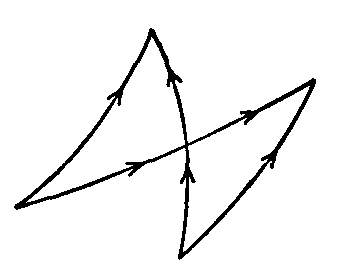
\includegraphics[width=25mm]{images/WRHfig1.png}
\end{center}

Soon after the publication of the Lectures, he became aware of its
imperfection as a manual of instruction, and he set himself to
prepare a second book on the model of Euclid's \emph{Elements}. He
estimated that it would fill 400 pages and take two years to
prepare; it amounted to nearly 800 closely printed pages and took
seven years. At times he would work for twelve hours on a stretch;
and he also suffered from anxiety as to the means of publication.
Trinity College advanced \pounds200, he paid \pounds50 out of his
own pocket, but when illness came upon him the expense of paper
and printing had mounted up to \pounds400. He was seized by an
acute attack of gout, from which, after several months of
suffering, he died on Sept.\ 2, 1865, in the 61st year of his age.

It is pleasant to know that this great mathematician received
during his last illness an honor from the United States, which
made him feel that he had realized the aim of his great labors.
While the war between the North and South was in progress, the
National Academy of Sciences was founded, and the news which came
to Hamilton was that he had been elected one of ten foreign
members, and that his name had been voted to occupy the specially
honorable position of first on the list. Sir William Rowan
Hamilton was thus the first foreign associate of the National
Academy of Sciences of the United States.

As regards religion Hamilton was deeply reverential in nature. He
was born and brought up in the Church of England, which was then
the established Church in Ireland. He lived in the time of the
Oxford movement, and for some time he sympathized with it; but
when several of his friends, among them the brother of Miss
De~Vere, passed over into the Roman Catholic Church, he modified
his opinion of the movement and remained Protestant to the end.

The immense intellectual activity of Hamilton, especially during
the years when he was engaged on the enormous labor of writing the
\emph{Elements of Quaternions}, made him a recluse, and
necessarily took away from his power of attending to the practical
affairs of life. Some said that however great a master of pure
time he might be he was not a master of sublunary time. His
neighbors also took advantage of his goodness of heart.
Surrounding the house there is an extensive lawn affording good
pasture, and on it Hamilton pastured a cow. A neighbor advised
Hamilton that his cow would be much better contented by having
another cow for company and bargained with Hamilton to furnish the
companion provided Hamilton paid something like a dollar per
month.

Here is Hamilton's own estimate of himself. ``I have very long
admired Ptolemy's description of his great astronomical master,
Hipparchus, as \selectlanguage{greek}>an'hr fil'oponos ka`i
filal'hjhc\selectlanguage{english}; a labor-loving and
truth-loving man. Be such my epitaph.''

Hamilton's family consisted of two sons and one daughter. At the
time of his death, the \emph{Elements of Quaternions} was all
finished excepting one chapter. His eldest son, William Edwin
Hamilton, wrote a preface, and the volume was published at the
expense of Trinity College, Dublin. Only 500 copies were printed,
and many of those were presented. In consequence it soon became a
scarce book, and as much as \$35.00 has been paid for a copy. A
new edition, in two volumes, is now being published by Prof.\
Joly, his successor in Dunsink Observatory.

\chapter [George Boole (1815-1864)]{GEORGE
BOOLE\footnote{This Lecture was delivered April 19,
1901.---\textsc{Editors.}}}

\large\begin{center}{(1815-1864)}\end{center}\normalsize

George Boole was born at Lincoln, England, on the 2d of November,
1815. His father, a tradesman of very limited means, was attached
to the pursuit of science, particularly of mathematics, and was
skilled in the construction of optical instruments. Boole received
his elementary education at the National School of the city, and
afterwards at a commercial school; but it was his father who
instructed him in the elements of mathematics, and also gave him a
taste for the construction and adaptation of optical instruments.
However, his early ambition did not urge him to the further
prosecution of mathematical studies, but rather to becoming
proficient in the ancient classical languages. In this direction
he could receive no help from his father, but to a friendly
bookseller of the neighborhood he was indebted for instruction in
the rudiments of the Latin Grammar. To the study of Latin he soon
added that of Greek without any external assistance; and for some
years he perused every Greek or Latin author that came within his
reach. At the early age of twelve his proficiency in Latin made
him the occasion of a literary controversy in his native city. He
produced a metrical translation of an ode of Horace, which his
father in the pride of his heart inserted in a local journal,
stating the age of the translator. A neighboring school-master
wrote a letter to the journal in which he denied, from internal
evidence, that the version could have been the work of one so
young. In his early thirst for knowledge of languages and ambition
to excel in verse he was like Hamilton, but poor Boole was much
more heavily oppressed by the \emph{res angusta domi}---the hard
conditions of his home. Accident discovered to him certain defects
in his methods of classical study, inseparable from the want of
proper early training, and it cost him two years of incessant
labor to correct them.

Between the ages of sixteen and twenty he taught school as an
assistant teacher, first at Doncaster in Yorkshire, afterwards at
Waddington near Lincoln; and the leisure of these years he devoted
mainly to the study of the principal modern languages, and of
patristic literature with the view of studying to take orders in
the Church. This design, however, was not carried out, owing to
the financial circumstances of his parents and some other
difficulties. In his twentieth year he decided on opening a school
on his own account in his native city; thenceforth he devoted all
the leisure he could command to the study of the higher
mathematics, and solely with the aid of such books as he could
procure. Without other assistance or guide he worked his way
onward, and it was his own opinion that he had lost five years of
educational progress by his imperfect methods of study, and the
want of a helping hand to get him over difficulties. No doubt it
cost him much time; but when he had finished studying he was
already not only learned but an experienced investigator.

We have seen that at this time (1835) the great masters of
mathematical analysis wrote in the French language; and Boole was
naturally led to the study of the \emph{M\'ecanique celeste} of
Laplace, and the \emph{M\'ecanique analytique} of Lagrange. While
studying the latter work he made notes from which there eventually
emerged his first mathematical memoir, entitled, ``On certain
theorems in the calculus of variations.'' By the same works his
attention was attracted to the transformation of homogeneous
functions by linear substitutions, and in the course of his
subsequent investigations he was led to results which are now
regarded as the foundation of the modern Higher Algebra. In the
publication of his results he received friendly assistance from
D.~F.\ Gregory, a younger member of the Cambridge school, and
editor of the newly founded \emph{Cambridge Mathematical Journal}.
Gregory and other friends suggested that Boole should take the
regular mathematical course at Cambridge, but this he was unable
to do; he continued to teach school for his own support and that
of his aged parents, and to cultivate mathematical analysis in the
leisure left by a laborious occupation.

Duncan F.\ Gregory was one of a Scottish family already
distinguished in the annals of science. His grandfather was James
Gregory, the inventor of the refracting telescope and discoverer
of a convergent series for $\pi$. A cousin of his father was David
Gregory, a special friend and fellow worker of Sir Isaac Newton.
D.~F.\ Gregory graduated at Cambridge, and after graduation he
immediately turned his attention to the logical foundations of
analysis. He had before him Peacock's theory of algebra, and he
knew that in the analysis as developed by the French school there
were many remarkable phenomena awaiting explanation; particularly
theorems which involved what was called the separation of symbols.
He embodied his results in a paper ``On the real Nature of
symbolical Algebra'' which was printed in the \emph{Transactions}
of the Royal Society of Edinburgh.

Boole became a master of the method of separation of symbols, and
by attempting to apply it to the solution of differential
equations with variable coefficients was led to devise a general
method in analysis. The account of it was printed in the
\emph{Transactions} of the Royal Society of London, and brought
its author a Royal medal. Boole's study of the separation of
symbols naturally led him to a study of the foundations of
analysis, and he had before him the writings of Peacock, Gregory
and De~Morgan. He was led to entertain very wide views of the
domain of mathematical analysis; in fact that it was coextensive
with exact analysis, and so embraced formal logic. In 1848, as we
have seen, the controversy arose between Hamilton and De~Morgan
about the quantification of terms; the general interest which that
controversy awoke in the relation of mathematics to logic induced
Boole to prepare for publication his views on the subject, which
he did that same year in a small volume entitled
\emph{Mathematical Analysis of Logic}.

About this time what are denominated the Queen's Colleges of
Ireland were instituted at Belfast, Cork and Galway; and in 1849
Boole was appointed to the chair of mathematics in the Queen's
College at Cork. In this more suitable environment he set himself
to the preparation of a more elaborate work on the mathematical
analysis of logic. For this purpose he read extensively books on
psychology and logic, and as a result published in 1854 the work
on which his fame chiefly rests---``An Investigation of the Laws
of Thought, on which are founded the mathematical theories of
logic and probabilities.'' Subsequently he prepared textbooks on
\emph{Differential Equations} and \emph{Finite Differences}; the
former of which remained the best English textbook on its subject
until the publication of Forsyth's \emph{Differential Equations}.

Prefixed to the \emph{Laws of Thought} is a dedication to Dr.\
Ryall, Vice-President and Professor of Greek in the same College.
In the following year, perhaps as a result of the dedication, he
married Miss Everest, the niece of that colleague. Honors came:
Dublin University made him an LL.D., Oxford a D.C.L.; and the
Royal Society of London elected him a Fellow. But Boole's career
was cut short in the midst of his usefulness and scientific
labors. One day in 1864 he walked from his residence to the
College, a distance of two miles, in a drenching rain, and
lectured in wet clothes. The result was a feverish cold which soon
fell upon his lungs and terminated his career on December 8, 1864,
in the 50th year of his age.

De~Morgan was the man best qualified to judge of the value of
Boole's work in the field of logic; and he gave it generous praise
and help. In writing to the Dublin Hamilton he said, ``I shall be
glad to see his work (\emph{Laws of Thought}) out, for he has, I
think, got hold of the true connection of algebra and logic.'' At
another time he wrote to the same as follows: ``All metaphysicians
except you and I and Boole consider mathematics as four books of
Euclid and algebra up to quadratic equations.'' We might infer
that these three contemporary mathematicians who were likewise
philosophers would form a triangle of friends. But it was not so;
Hamilton was a friend of De~Morgan, and De~Morgan a friend of
Boole; but the relation of \emph{friend}, although convertible, is
not necessarily transitive. Hamilton met De~Morgan only once in
his life, Boole on the other hand with comparative frequency; yet
he had a voluminous correspondence with the former extending over
20 years, but almost no correspondence with the latter.
De~Morgan's investigations of double algebra and triple algebra
prepared him to appreciate the quaternions, whereas Boole was too
much given over to the symbolic theory to appreciate geometric
algebra.

Hamilton's biography has appeared in three volumes, prepared by
his friend Rev.\ Charles Graves; De~Morgan's biography has
appeared in one volume, prepared by his widow; of Boole no
biography has appeared. A biographical notice of Boole was written
for the \emph{Proceedings} of the Royal Society of London by his
friend the Rev.\ Robert Harley, and it is to it that I am indebted
for most of my biographical data. Last summer when in England I
learned that the reason why no adequate biography of Boole had
appeared was the unfortunate temper and lack of sound judgment of
his widow. Since her husband's death Mrs.\ Boole has published a
paradoxical book of the false kind worthy of a notice in
De~Morgan's \emph{Budget}.

The work done by Boole in applying mathematical analysis to logic
necessarily led him to consider the general question of how
reasoning is accomplished by means of symbols. The view which he
adopted on this point is stated at page 68 of the \emph{Laws of
Thought}. ``The conditions of valid reasoning by the aid of
symbols, are: \emph{First}, that a fixed interpretation be
assigned to the symbols employed in the expression of the data;
and that the laws of the combination of those symbols be correctly
determined from that interpretation; \emph{Second}, that the
formal processes of solution or demonstration be conducted
throughout in obedience to all the laws determined as above,
without regard to the question of the interpretability of the
particular results obtained; \emph{Third}, that the final result
be interpretable in form, and that it be actually interpreted in
accordance with that system of interpretation which has been
employed in the expression of the data.'' As regards these
conditions it may be observed that they are very different from
the formalist view of Peacock and De~Morgan, and that they incline
towards a realistic view of analysis, as held by Hamilton. True he
speaks of interpretation instead of meaning, but it is a fixed
interpretation; and the rules for the processes of solution are
not to be chosen arbitrarily, but are to be found out from the
particular system of interpretation of the symbols.

It is Boole's second condition which chiefly calls for study and
examination; respecting it he observes as follows: ``The principle
in question may be considered as resting upon a general law of the
mind, the knowledge of which is not given to us \emph{a priori},
that is, antecedently to experience, but is derived, like the
knowledge of the other laws of the mind, from the clear
manifestation of the general principle in the particular instance.
A single example of reasoning, in which symbols are employed in
obedience to laws founded upon their interpretation, but without
any sustained reference to that interpretation, the chain of
demonstration conducting us through intermediate steps which are
not interpretable to a final result which is interpretable, seems
not only to establish the validity of the particular application,
but to make known to us the general law manifested therein. No
accumulation of instances can properly add weight to such
evidence. It may furnish us with clearer conceptions of that
common element of truth upon which the application of the
principle depends, and so prepare the way for its reception. It
may, where the immediate force of the evidence is not felt, serve
as a verification, \emph{a posteriori}, of the practical validity
of the principle in question. But this does not affect the
position affirmed, viz., that the general principle must be seen
in the particular instance---seen to be general in application as
well as true in the special example. The employment of the
uninterpretable symbol $\sqrt{-1}$ in the intermediate processes
of trigonometry furnishes an illustration of what has been said. I
apprehend that there is no mode of explaining that application
which does not covertly assume the very principle in question. But
that principle, though not, as I conceive, warranted by formal
reasoning based upon other grounds, seems to deserve a place among
those axiomatic truths which constitute in some sense the
foundation of general knowledge, and which may properly be
regarded as expressions of the mind's own laws and constitution.''

We are all familiar with the fact that algebraic reasoning may be
conducted through intermediate equations without requiring a
sustained reference to the meaning of these equations; but it is
paradoxical to say that these equations can, in any case, have no
meaning or interpretation. It may not be necessary to consider
their meaning, it may even be difficult to find their meaning, but
that they have a meaning is a dictate of common sense. It is
entirely paradoxical to say that, as a general process, we can
start from equations having a meaning, and arrive at equations
having a meaning by passing through equations which have no
meaning. The particular instance in which Boole sees the truth of
the paradoxical principle is the successful employment of the
uninterpretable symbol $\sqrt{-1}$ in the intermediate processes
of trigonometry. So soon then as this symbol is interpreted, or
rather, so soon as its meaning is demonstrated, the evidence for
the principle fails, and Boole's transcendental logic falls.

In the algebra of quantity we start from elementary symbols
denoting numbers, but are soon led to compound forms which do not
reduce to numbers; so in the algebra of logic we start from
elementary symbols denoting classes, but are soon introduced to
compound expressions which cannot be reduced to simple classes.
Most mathematical logicians say, Stop, we do not know what this
combination means. Boole says, It may be meaningless, go ahead all
the same. The design of the \emph{Laws of Thought} is stated by
the author to be to investigate the fundamental laws of those
operations of the mind by which reasoning is performed; to give
expression to them in the symbolical language of a Calculus, and
upon this foundation to establish the Science of Logic and
construct its method; to make that method itself the basis of a
general method for the application of the mathematical doctrine of
Probabilities; and, finally to collect from the various elements
of truth brought to view in the course of these inquiries some
probable intimations concerning the nature and constitution of the
human mind.

Boole's inventory of the symbols required in the algebra of logic
is as follows: \emph{first}, Literal symbols, as $x$, $y$, etc.,
representing things as subjects of our conceptions; \emph{second},
Signs of operation, as $+$, $-$, $\times$, standing for those
operations of the mind by which the conceptions of things are
combined or resolved so as to form new conceptions involving the
same elements; \emph{third}, The sign of identity $=$; not
equality merely, but identity which involves equality. The symbols
$x$, $y$, etc., are used to denote classes; and it is one of
Boole's maxims that substantives and adjectives alike denote
classes. ``They may be regarded,'' he says, ``as differing only in
this respect, that the former expresses the substantive existence
of the individual thing or things to which it refers, the latter
implies that existence. If we attach to the adjective the
universally understood subject, `being' or `thing,' it becomes
virtually a substantive, and may for all the essential purposes of
reasoning be replaced by the substantive.'' Let us then agree to
represent the class of individuals to which a particular name is
applicable by a single letter as $x$. If the name is \emph{men}
for instance, let $x$ represent \emph{all men}, or the class
\emph{men}. Again, if an adjective, as \emph{good}, is employed as
a term of description, let us represent by a letter, as $y$, all
things to which the description \emph{good} is applicable, that
is, \emph{all good things} or the class \emph{good things}. Then
the combination $yx$ will represent \emph{good men}.

Boole's symbolic logic was brought to my notice by Professor Tait,
when I was a student in the physical laboratory of Edinburgh
University. I studied the \emph{Laws of Thought} and I found that
those who had written on it regarded the method as highly
mysterious; the results wonderful, but the processes obscure. I
reduced everything to diagram and model, and I ventured to publish
my views on the subject in a small volume called \emph{Principles
of the Algebra of Logic}; one of the chief points I made is the
philological and analytical difference between the substantive and
the adjective. What I said was that the word \emph{man} denotes a
class, but the word \emph{white} does not; in the former a
definite unit-object is specified, in the latter no unit-object is
specified. We can exhibit a type of a \emph{man}, we cannot
exhibit a type of a \emph{white}.

The identification of the substantive and adjective on the one
hand and their discrimination on the other hand, lead to different
conceptions of what De~Morgan called the \emph{universe}. Boole's
conception of the Universe is as follows (\emph{Laws of Thought},
p. 42): ``In every discourse, whether of the mind conversing with
its own thoughts, or of the individual in his intercourse with
others, there is an assumed or expressed limit within which the
subjects of its operation are confined. The most unfettered
discourse is that in which the words we use are understood in the
widest possible application, and for them the limits of discourse
are coextensive with those of the universe itself. But more
usually we confine ourselves to a less spacious field. Sometimes
in discoursing of men we imply (without expressing the limitation)
that it is of men only under certain circumstances and conditions
that we speak, as of civilized men, or of men in the vigor of
life, or of men under some other condition or relation. Now,
whatever may be the extent of the field within which all the
objects of our discourse are found, that field may properly be
termed the universe of discourse.''

Another view leads to the conception of the Universe as a
collection of homogeneous units, which may be finite or infinite
in number; and in a particular problem the mind considers the
relation of identity between different groups of this collection.
This \emph{universe} corresponds to \emph{the series of events},
in the theory of Probability; and the characters correspond to the
different ways in which the event may happen. The difference is
that the Algebra of Logic considers necessary data and relations;
while the theory of Probability considers probable data and
relations. I will explain the elements of Boole's method on this
theory.

\begin{center}
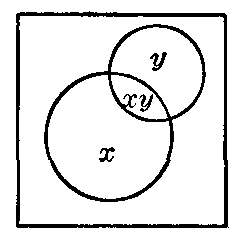
\includegraphics[width=25mm]{images/GBfig1.png} \\
\footnotesize \textsc{Fig.\ 1.} \normalsize
\end{center}

The square is a collection of points: it may serve to represent
any collection of homogeneous units, whether finite or infinite in
number, that is, the universe of the problem. Let $x$ denote
\emph{inside the left-hand circle}, and $y$ \emph{inside the
right-hand circle}. $Uxy$ will denote the points inside both
circles (Fig.\ 1). In arithmetical value $x$ may range from $1$ to
$0$; so also $y$; while $xy$ cannot be greater than $x$ or $y$, or
less than $0$ or $x+y-1$. This last is the principle of the
syllogism. From the co-ordinate nature of the operations $x$ and
$y$, it is evident that $Uxy = Uyx$; but this is a different thing
from commuting, as Boole does, the relation of $U$ and $x$, which
is not that of co-ordination, but of subordination of $x$ to $U$,
and which is properly denoted by writing $U$ first.

Suppose $y$ to be the same character as $x$; we will then always
have $Uxx=Ux$; that is, an elementary selective symbol $x$ is
always such that $x^2 = x$. These are but the symbols of ordinary
algebra which satisfy this relation, namely $1$ and $0$; these are
also the extreme selective symbols \emph{all} and \emph{none}. The
law in question was considered Boole's paradox; it plays a very
great part in the development of his method.

\begin{center}
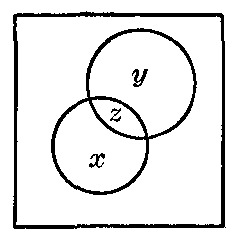
\includegraphics[width=25mm]{images/GBfig2.png} \\
\footnotesize \textsc{Fig.\ 2.} \normalsize
\end{center}

Let $Uxy = Uz$, where $=$ means \emph{identical with}, not
\emph{equal to}; we may write $xy = z$, leaving the $U$ to be
understood. It does not mean that the combination of characters
$xy$ is identical with the character $z$; but that those points
which have the characters $x$ and $y$ are identical with the
points which have the character $z$ (Fig. 2). From $xy = z$, we
derive $x = \frac{1}{y} z$; what is the meaning of this
expression? We shall return to the question, after we have
considered $+$ and $-$.

\begin{center}
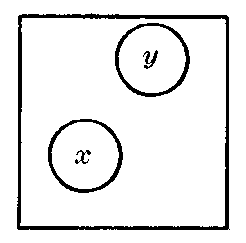
\includegraphics[width=25mm]{images/GBfig3.png} \quad
   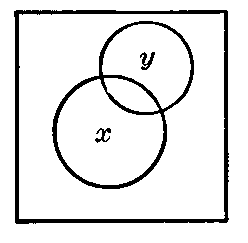
\includegraphics[width=25mm]{images/GBfig4.png} \\
\footnotesize \textsc{Fig.\ 3} \qquad \qquad \qquad
   \textsc{Fig.\ 4} \normalsize
\end{center}

Let us now consider the expression $U(x+y)$. If the $x$ points and
the $y$ points are outside of one another, it means the sum of the
$x$ points and the $y$ points (Fig.\ 3). So far all are agreed. But
suppose that the $x$ points and the $y$ points are partially
identical (Fig.\ 4); then there arises difference of opinion. Boole
held that the common points must be taken twice over, or in other
words that the symbols $x$ and $y$ must be treated all the same as
if they were independent of one another; otherwise, he held, no
general analysis is possible. $U(x+y)$ will not in general denote
a single class of points; it will involve in general a
duplication.

\begin{center}
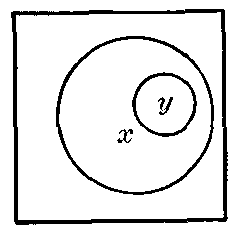
\includegraphics[width=25mm]{images/GBfig5.png} \\
\footnotesize \textsc{Fig.\ 5.} \normalsize
\end{center}

Similarly, Boole held that the expression $U(x-y)$ does not
involve the condition of the $Uy$ being wholly included in the
$Ux$ (Fig.\ 5). If that condition is satisfied, $U(x-y)$ denotes a
simple class; namely, the $Ux$'s \emph{without} the $Uy$'s. But
when there is partial coincidence (as in Fig.\ 4), the common
points will be cancelled, and the result will be the $Ux$'s which
are not $y$ taken positively and the $Uy$'s which are not $x$
taken negatively. In Boole's view $U(x-y)$ was in general an
intermediate uninterpretable form, which might be used in
reasoning the same way as analysts used $\sqrt{-1}$.

Most of the mathematical logicians who have come after Boole are
men who would have stuck at the impossible subtraction in ordinary
algebra. They say virtually, ``How can you throw into a heap the
same things twice over; and how can you take from a heap things
that are not there.'' Their great principle is the impossibility of
taking the pants from a Highlander. Their only conception of the
analytical processes of addition and subtraction is throwing into
a heap and taking out of a heap. It does not occur to them that
the processes of algebra are \emph{ideal}, and not subject to
gross material restrictions.

If $x+y$ denotes a quality without duplication, it will satisfy
the condition
\begin{align*}
                   (x+y)^2 &= x+y, \\
               x^2+2xy+y^2 &= x+y, \\
  \text{but } x^2 = x, y^2 &= y,   \\
            \therefore 2xy &= 0.
\end{align*}

Similarly, if $x-y$ denote a simple quality, then
\begin{align*}
                 (x-y)^2 &= x-y, \\
             x^2+y^2-2xy &= x-y, \\
      x^2 = x, \quad y^2 &= y,   \\
\text{therefore, } y-2xy &=-y,   \\
            \therefore y &= xy.
\end{align*}

In other words, the $Uy$ must be included in the $Ux$ (Fig.\ 5).
Here we have assumed that the law of signs is the same as in
ordinary algebra, and the result comes out correct.

Suppose $Uz$=$Uxy$; then $Ux=U\frac{1}{y}z$. How are the $Ux$'s
related to the $Uy$'s, and the Uz's? From the diagram (in Fig.\ 2)
we see that the $Ux$'s are identical with all the $Uyz$'s together
with an indefinite portion of the $U$'s, which are neither $y$ nor
$z$. Boole discovered a general method for finding the meaning of
any function of elementary logical symbols, which applied to the
above case, is as follows:

When $y$ is an elementary symbol,
\begin{align*}
                  1&=y+(1-y). \\
\text{Similarly } 1&=z+(1-z). \\
       \therefore 1&=yz+y(1-z)+(1-y)z+(1-y)(1-z),
\end{align*}
\noindent which means that the $U$'s either have both qualities
$y$ and $z$, or $y$ but not $z$, or $z$ but not $y$, or neither
$y$ and $z$. Let
\begin{equation*}
\frac{1}{y}z = Ayz + By(1-z) + C(1-y)z + D(1-y)(1-z),
\end{equation*}
\noindent it is required to determine the coefficients $A$, $B$,
$C$, $D$. Suppose $y=1$, $z=1$; then $1=A$. Suppose $y=1$, $z=0$,
then $0=B$. Suppose $y=0$, $z=1$; then $\frac{1}{0}=C$, and $C$ is
infinite; therefore $(1-y)z=0$; which we see to be true from the
diagram. Suppose $y=0$, $z=0$; then $\frac{0}{0}=D$, or $D$ is
indeterminate. Hence
\begin{equation*}
\frac{1}{y}z = yz+\text{an indefinite portion of }(1-y)(1-z).
\end{equation*}

\begin{center}
*\hspace{1cm}*\hspace{1cm}*\hspace{1cm}*\hspace{1cm}*
\end{center}

Boole attached great importance to the index law $x^2=x$. He held
that it expressed a law of thought, and formed the characteristic
distinction of the operations of the mind in its ordinary
discourse and reasoning, as compared with its operations when
occupied with the general algebra of quantity. It makes possible,
he said, the solution of a quintic or equation of higher degree,
when the symbols are logical. He deduces from it the axiom of
metaphysicians which is termed the principle of contradiction, and
which affirms that it is impossible for any being to possess a
quality, and at the same time not to possess it. Let $x$ denote an
elementary quality applicable to the universe $U$; then $1 - x$
denotes the absence of that quality. But if $x^{2} = x$, then $0 =
x - x^{2}, 0 = x(1 - x)$, that is, from $Ux^{2}=Ux$ we deduce
$Ux(1 - x) = 0$.

He considers $x(1 - x) = 0$ as an expression of the principle of
contradiction. He proceeds to remark: ``The above interpretation
has been introduced not on account of its immediate value in the
present system, but as an illustration of a significant fact in
the philosophy of the intellectual powers, viz., that what has
been commonly regarded as the fundamental axiom of metaphysics is
but the consequence of a law of thought, mathematical in its form.
I desire to direct attention also to the circumstance that the
equation in which that fundamental law of thought is expressed is
an equation of the second degree. Without speculating at all in
this chapter upon the question whether that circumstance is
necessary in its own nature, we may venture to assert that if it
had not existed, the whole procedure of the understanding would
have been different from what it is.''

We have seen that De~Morgan investigated long and published much
on mathematical logic. His logical writings are characterized by a
display of many symbols, new alike to logic and to mathematics; in
the words of Sir W.\ Hamilton of Edinburgh, they are ``horrent
with mysterious spicul\ae{}.'' It was the great merit of Boole's
work that he used the immense power of the ordinary algebraic
notation as an exact language and proved its power for making
ordinary language more exact. De~Morgan could well appreciate the
magnitude of the feat, and he gave generous testimony to it as
follows:

``Boole's system of logic is but one of many proofs of genius and
patience combined. I might legitimately have entered it among my
\emph{paradoxes}, or things counter to general opinion: but it is
a paradox which, like that of Copernicus, excited admiration from
its first appearance. That the symbolic processes of algebra,
invented as tools of numerical calculation, should be competent to
express every act of thought, and to furnish the grammar and
dictionary of an all-containing system of logic, would not have
been believed until it was proved. When Hobbes, in the time of the
Commonwealth, published his ``Computation or Logique'' he had a
remote glimpse of some of the points which are placed in the light
of day by Mr.\ Boole. The unity of the forms of thought in all the
applications of reason, however remotely separated, will one day
be matter of notoriety and common wonder: and Boole's name will be
remembered in connection with one of the most important steps
towards the attainment of this knowledge.''


\chapter [Arthur Cayley (1821-1895)]{ARTHUR
CAYLEY\footnote{This Lecture was delivered April 20,
1901.---\textsc{Editors.}}}

\large\begin{center}{(1821-1895)}\end{center}\normalsize

Arthur Cayley was born at Richmond in Surrey, England, on August
16, 1821. His father, Henry Cayley, was descended from an ancient
Yorkshire family, but had settled in St.\ Petersburg, Russia, as a
merchant. His mother was Maria Antonia Doughty, a daughter of
William Doughty; who, according to some writers, was a Russian;
but her father's name indicates an English origin. Arthur spent
the first eight years of his life in St.\ Petersburg. In 1829 his
parents took up their permanent abode at Blackheath, near London;
and Arthur was sent to a private school. He early showed great
liking for, and aptitude in, numerical calculations. At the age of
14 he was sent to King's College School, London; the master of
which, having observed indications of mathematical genius, advised
the father to educate his son, not for his own business, as he had
at first intended, but to enter the University of Cambridge.

At the unusually early age of 17 Cayley began residence at Trinity
College, Cambridge. As an undergraduate he had generally the
reputation of being a mere mathematician; his chief diversion was
novel-reading. He was also fond of travelling and mountain
climbing, and was a member of the Alpine Club. The cause of the
Analytical Society had now triumphed, and the \emph{Cambridge
Mathematical Journal} had been instituted by Gregory and Leslie
Ellis. To this journal, at the age of twenty, Cayley contributed
three papers, on subjects which had been suggested by reading the
\emph{M\'ecanique analytique} of Lagrange and some of the works of
Laplace. We have already noticed how the works of Lagrange and
Laplace served to start investigation in Hamilton and Boole.
Cayley finished his undergraduate course by winning the place of
Senior Wrangler, and the first Smith's prize. His next step was to
take the M.A.\ degree, and win a Fellowship by competitive
examination. He continued to reside at Cambridge for four years;
during which time he took some pupils, but his main work was the
preparation of 28 memoirs to the \emph{Mathematical Journal}. On
account of the limited tenure of his fellowship it was necessary
to choose a profession; like De~Morgan, Cayley chose the law, and
at 25 entered at Lincoln's Inn, London. He made a specialty of
conveyancing and became very skilled at the work; but he regarded
his legal occupation mainly as the means of providing a
livelihood, and he reserved with jealous care a due portion of his
time for mathematical research. It was while he was a pupil at the
bar that he went over to Dublin for the express purpose of hearing
Hamilton's lectures on Quaternions. He sat alongside of Salmon
(now provost of Trinity College, Dublin) and the readers of
Salmon's books on Analytical Geometry know how much their author
was indebted to his correspondence with Cayley in the matter of
bringing his textbooks up to date. His friend Sylvester, his
senior by five years at Cambridge, was then an actuary, resident
in London; they used to walk together round the courts of
Lincoln's Inn, discussing the theory of invariants and covariants.
During this period of his life, extending over fourteen years,
Cayley produced between two and three hundred papers.

At Cambridge University the ancient professorship of pure
mathematics is denominated the Lucasian, and is the chair which
was occupied by Sir Isaac Newton. About 1860 certain funds
bequeathed by Lady Sadleir to the University, having become
useless for their original purpose, were employed to establish
another professorship of pure mathematicas, called the Sadlerian.
The duties of the new professor were defined to be ``to explain
and teach the principles of pure mathematics and to apply himself
to the advancement of that science.'' To this chair Cayley was
elected when 42 years old. He gave up a lucrative practice for a
modest salary; but he never regretted the exchange, for the chair
at Cambridge enabled him to end the divided allegiance between law
and mathematics, and to devote his energies to the pursuit which
he liked best. He at once married and settled down in Cambridge.
More fortunate than Hamilton in his choice, his home life was one
of great happiness. His friend and fellow investigator, Sylvester,
once remarked that Cayley had been much more fortunate than
himself; that they both lived as bachelors in London, but that
Cayley had married and settled down to a quiet and peaceful life
at Cambridge; whereas he had never married, and had been fighting
the world all his days. The remark was only too true (as may be
seen in the lecture on Sylvester).

At first the teaching duty of the Sadlerian professorship was
limited to a course of lectures extending over one of the terms of
the academic year; but when the University was reformed about
1886, and part of the college funds applied to the better
endowment of the University professors, the lectures were extended
over two terms. For many years the attendance was small, and came
almost entirely from those who had finished their career of
preparation for competitive examinations; after the reform the
attendance numbered about fifteen. The subject lectured on was
generally that of the memoir on which the professor was for the
time engaged.

The other duty of the chair---the advancement of mathematical
science was---discharged in a handsome manner by the long series
of memoirs which he published, ranging over every department of
pure mathematics. But it was also discharged in a much less
obtrusive way; he became the standing referee on the merits of
mathematical papers to many societies both at home and abroad.
Many mathematicians, of whom Sylvester was an example, find it
irksome to study what others have written, unless, perchance, it
is something dealing directly with their own line of work. Cayley
was a man of more cosmopolitan spirit; he had a friendly sympathy
with other workers, and especially with young men making their
first adventure in the field of mathematical research. Of referee
work he did an immense amount; and of his kindliness to young
investigators I can speak from personal experience. Several papers
which I read before the Royal Society of Edinburgh on the Analysis
of Relationships were referred to him, and he recommended their
publication. Soon after I was invited by the Anthropological
Society of London to address them on the subject, and while there,
I attended a meeting of the Mathematical Society of London. The
room was small, and some twelve mathematicians were assembled
round a table, among whom was Prof.\ Cayley, as became evident to
me from the proceedings. At the close of the meeting Cayley gave
me a cordial handshake and referred in the kindest terms to my
papers which he had read. He was then about 60 years old,
considerably bent, and not filling his clothes. What was most
remarkable about him was the active glance of his gray eyes and
his peculiar boyish smile.

In 1876 he published a \emph{Treatise on Elliptic Functions},
which was his only book. He took great interest in the movement
for the University education of women. At Cambridge the women's
colleges are Girton and Newnham. In the early days of Girton
College he gave direct help in teaching, and for some years he was
chairman of the council of Newnham College, in the progress of
which he took the keenest interest to the last. His mathematical
investigations did not make him a recluse; on the contrary he was
of great practical usefulness, especially from his knowledge of
law, in the administration of the University.

In 1872 he was made an honorary fellow of Trinity College, and
three years later an ordinary fellow, which meant stipend as well
as honor. About this time his friends subscribed for a
presentation portrait, which now hangs on the side wall of the
dining hall of Trinity College, next to the portrait of James
Clerk Maxwell, while on the end wall, behind the high table, hang
the more ancient portraits of Sir Isaac Newton and Lord Bacon of
Verulam. In the portrait Cayley is represented as seated at a
desk, quill in hand, after the mode in which he used to write out
his mathematical investigations. The investigation, however, was
all thought out in his mind before he took up the quill.

Maxwell was one of the greatest electricians of the nineteenth
century. He was a man of philosophical insight and poetical power,
not unlike Hamilton, but differing in this, that he was no orator.
In that respect he was more like Goldsmith, who ``could write like
an angel, but only talked like poor poll.'' Maxwell wrote an
address to the committee of subscribers who had charge of the
Cayley portrait fund, wherein the scientific poet with his pen
does greater honor to the mathematician than the artist, named
Dickenson, could do with his brush. Cayley had written on space of
\emph{n} dimensions, and the main point in the address is derived
from the artist's business of depicting on a plane what exists in
space:

\begin{verse}
O wretched race of men, to space confined! \\
What honor can ye pay to him whose mind \\
To that which lies beyond hath penetrated? \\
The symbols he hath formed shall sound his praise, \\
And lead him on through unimagined ways \\
To conquests new, in worlds not yet created.

First, ye Determinants, in ordered row \\
And massive column ranged, before him go, \\
To form a phalanx for his safe protection. \\
Ye powers of the $n$th root of $-1$! \\
Around his head in endless cycles run, \\
As unembodied spirits of direction.

And you, ye undevelopable scrolls! \\
Above the host where your emblazoned rolls, \\
Ruled for the record of his bright inventions. \\
Ye cubic surfaces! by threes and nines \\
Draw round his camp your seven and twenty lines \\
The seal of Solomon in three dimensions.

March on, symbolic host! with step sublime, \\
Up to the flaming bounds of Space and Time! \\
There pause, until by Dickenson depicted \\
In two dimensions, we the form may trace \\
Of him whose soul, too large for vulgar space, \\
In $n$ dimensions flourished unrestricted.
\end{verse}

The verses refer to the subjects investigated in several of
Cayley's most elaborate memoirs; such as, Chapters on the
Analytical Geometry of \emph{n} dimensions; On the theory of
Determinants; Memoir on the theory of Matrices; Memoirs on skew
surfaces, otherwise Scrolls; On the delineation of a Cubic Scroll,
etc.

In 1881 he received from the Johns Hopkins University, Baltimore,
where Sylvester was then professor of mathematics, an invitation
to deliver a course of lectures. He accepted the invitation, and
lectured at Baltimore during the first five months of 1882 on the
subject of the \emph{Abelian and Theta Functions}.

The next year Cayley came prominently before the world, as
President of the British Association for the Advancement of
Science. The meeting was held at Southport, in the north of
England. As the President's address is one of the great popular
events of the meeting, and brings out an audience of general
culture, it is usually made as little technical as possible.
Hamilton was the kind of mathematician to suit such an occasion,
but he never got the office, on account of his occasional breaks.
Cayley had not the oratorical, the philosophical, or the poetical
gifts of Hamilton, but then he was an eminently safe man. He took
for his subject the Progress of Pure Mathematics; and he opened
his address in the following na\"{\i}ve manner: ``I wish to speak
to you to-night upon Mathematics. I am quite aware of the
difficulty arising from the abstract nature of my subject; and if,
as I fear, many or some of you, recalling the providential
addresses at former meetings, should wish that you were now about
to have from a different President a discourse on a different
subject, I can very well sympathize with you in the feeling. But
be that as it may, I think it is more respectful to you that I
should speak to you upon and do my best to interest you in the
subject which has occupied me, and in which I am myself most
interested. And in another point of view, I think it is right that
the address of a president should be on his own subject, and that
different subjects should be thus brought in turn before the
meetings. So much the worse, it may be, for a particular meeting:
but the meeting is the individual, which on evolution principles,
must be sacrificed for the development of the race.'' I daresay
that after this introduction, all the evolution philosophers
listened to him attentively, whether they understood him or not.
But Cayley doubtless felt that he was addressing not only the
popular audience then and there before him, but the mathematicians
of distant places and future times; for the address is a valuable
historical review of various mathematical theories, and is
characterized by freshness, independence of view, suggestiveness,
and learning.

In 1889 the Cambridge University Press requested him to prepare
his mathematical papers for publication in a collected form---a
request which he appreciated very much. They are printed in
magnificent quarto volumes, of which seven appeared under his own
editorship. While editing these volumes, he was suffering from a
painful internal malady, to which he succumbed on January 26,
1895, in the 74th year of his age. When the funeral took place, a
great assemblage met in Trinity Chapel, comprising members of the
University, official representatives of Russia and America, and
many of the most illustrious philosophers of Great Britain.

The remainder of his papers were edited by Prof.\ Forsyth, his
successor in the Sadlerian chair. The Collected Mathematical
papers number thirteen quarto volumes, and contain 967 papers. His
writings are his best monument, and certainly no mathematician has
ever had his monument in grander style. De~Morgan's works would be
more extensive, and much more useful, but he did not have behind
him a University Press. As regards fads, Cayley retained to the
last his fondness for novel-reading and for travelling. He also
took special pleasure in paintings and architecture, and he
practised water-color painting, which he found useful sometimes in
making mathematical diagrams.

To the third edition of Tait's \emph{Elementary Treatise on
Quaternions}, Cayley contributed a chapter entitled ``Sketch of
the analytical theory of quaternions.'' In it the $\sqrt{-1}$
reappears in all its glory, and in entire, so it is said,
independence of $i$, $j$, $k$. The remarkable thing is that
Hamilton started with a quaternion theory of analysis, and that
Cayley should present instead an analytical theory of quaternions.
I daresay that Prof.\ Tait was sorry that he allowed the chapter
to enter his book, for in 1894 there arose a brisk discussion
between himself and Cayley on ``Coordinates versus Quaternions,''
the record of which is printed in the Proceedings of the Royal
Society of Edinburgh. Cayley maintained the position that while
coordinates are applicable to the whole science of geometry and
are the natural and appropriate basis and method in the science,
quaternions seemed a particular and very artificial method for
treating such parts of the science of three-dimensional geometry
as are most naturally discussed by means of the rectangular
coordinates $x$, $y$, $z$. In the course of his paper Cayley says:
``I have the highest admiration for the notion of a quaternion;
but, as I consider the full moon far more beautiful than any
moonlit view, so I regard the notion of a quaternion as far more
beautiful than any of its applications. As another illustration, I
compare a quaternion formula to a pocket-map---a capital thing to
put in one's pocket, but which for use must be unfolded: the
formula, to be understood, must be translated into coordinates.''
He goes on to say, ``I remark that the imaginary of ordinary
algebra---for distinction call this $\theta$---has no relation
whatever to the quaternion symbols $i$, $j$, $k$; in fact, in the
general point of view, all the quantities which present
themselves, are, or may be, complex values $a + \theta b$, or in
other words, say that a scalar quantity is in general of the form
$a + \theta b$. Thus quaternions do not properly present
themselves in plane or two-dimensional geometry at all; but they
belong essentially to solid or three-dimensional geometry, and
they are most naturally applicable to the class of problems which
in coordinates are dealt with by means of the three rectangular
coordinates $x$, $y$, $z$."

To the pocketbook illustration it may be replied that a set of
coordinates is an immense wall map, which you cannot carry about,
even though you should roll it up, and therefore is useless for
many important purposes. In reply to the arguments, it may be
said, \emph{first}, $\sqrt{-1}$ has a relation to the symbols $i$,
$j$, $k$, for each of these can be analyzed into a unit axis
multiplied by $\sqrt{-1}$; \emph{second}, as regards plane
geometry, the ordinary form of complex quantity is a degraded form
of the quaternion in which the constant axis of the plane is left
unspecified. Cayley took his illustrations from his experience as
a traveller. Tait brought forward an illustration from which you
might imagine he had visited the Bethlehem Iron Works, and hunted
tigers in India. He says, ``A much more natural and adequate
comparison would, it seems to me, liken Coordinate Geometry to a
steam-hammer, which an expert may employ on any destructive or
constructive work of one general kind, say the cracking of an
eggshell, or the welding of an anchor. But you must have your
expert to manage it, for without him it is useless. He has to toil
amid the heat, smoke, grime, grease, and perpetual din of the
suffocating engine-room. The work has to be brought to the hammer,
for it cannot usually be taken to its work. And it is not in
general, transferable; for each expert, as a rule, knows, fully
and confidently, the working details of his own weapon only.
Quaternions, on the other hand, are like the elephant's trunk,
ready at \emph{any} moment for \emph{anything}, be it to pick up a
crumb or a field-gun, to strangle a tiger, or uproot a tree;
portable in the extreme, applicable anywhere---alike in the
trackless jungle and in the barrack square---directed by a little
native who requires no special skill or training, and who can be
transferred from one elephant to another without much hesitation.
Surely this, which adapts itself to its work, is the grander
instrument. But then, \emph{it} is the natural, the other, the
artificial one.''

The reply which Tait makes, so far as it is an argument, is: There
are two systems of quaternions, the $i$, $j$, $k$ one, and another
one which Hamilton developed from it; Cayley knows the first only,
he himself knows the second; the former is an intensely artificial
system of imaginaries, the latter is the natural organ of
expression for quantities in space. Should a fourth edition of his
\emph{Elementary Treatise} be called for $i$, $j$, $k$ will
disappear from it, excepting in Cayley's chapter, should it be
retained. Tait thus describes the first system: ``Hamilton's
extraordinary \emph{Preface} to his first great book shows how
from Double Algebras, through Triplets, Triads, and Sets, he
finally reached Quaternions. This was the genesis of the
Quaternions of the forties, and the creature thus produced is
still essentially the Quaternion of Prof.\ Cayley. It is a
magnificent analytical conception; but it is nothing more than the
full development of the system of imaginaries $i$, $j$, $k$;
defined by the equations,
\begin{equation*}
i^{2} = j^{2} = k^{2} = ijk = -1,
\end{equation*}
\noindent with the associative, but \emph{not} the commutative,
law for the factors. The novel and splendid points in it were the
treatment of all directions in space as essentially alike in
character, and the recognition of the unit vector's claim to rank
also as a quadrantal versor. These were indeed inventions of the
first magnitude, and of vast importance. And here I thoroughly
agree with Prof.\ Cayley in his admiration. Considered as an
analytical system, based throughout on pure imaginaries, the
Quaternion method is elegant in the extreme. But, unless it had
been also something more, something very different and much higher
in the scale of development, I should have been content to admire
it;---and to pass it by.''

From ``the most intensely artificial of systems, arose, as if by
magic, an absolutely natural one'' which Tait thus further
describes. ``To me Quaternions are primarily a Mode of
Representation:---immensely superior to, but of essentially the
same kind of usefulness as, a diagram or a model. They are,
virtually, the thing represented; and are thus antecedent to, and
independent of, coordinates; giving, in general, all the main
relations, in the problem to which they are applied, without the
necessity of appealing to coordinates at all. Coordinates may,
however, easily be read into them:---when anything (such as
metrical or numerical detail) is to be gained thereby.
Quaternions, in a word, exist in space, and we have only to
recognize them:---but we have to invent or imagine coordinates of
all kinds.''

To meet the objection why Hamilton did not throw $i$, $j$, $k$
overboard, and expound the developed system, Tait says: ``Most
unfortunately, alike for himself and for his grand conception,
Hamilton's nerve failed him in the composition of his first great
volume. Had he then renounced, for ever, all dealings with $i$,
$j$, $k$, his triumph would have been complete. He spared Agog,
and the best of the sheep, and did not utterly destroy them. He
had a paternal fondness for $i$, $j$, $k$; perhaps also a not
unnatural liking for a meretricious title such as the mysterious
word \emph{Quaternion}; and, above all, he had an earnest desire
to make the utmost return in his power for the liberality shown
him by the authorities of Trinity College, Dublin. He had fully
recognized, and proved to others, that his $i$, $j$, $k$, were
mere excrescences and blots on his improved method:---but he
unfortunately considered that their continued (if only partial)
recognition was indispensable to the reception of his method by a
world steeped in---Cartesianism! Through the whole compass of each
of his tremendous volumes one can find traces of his desire to
avoid even an allusion to $i$, $j$, $k$, and along with them, his
sorrowful conviction that, should he do so, he would be left
without a single reader.''

To Cayley's presidential address we are indebted for information
about the view which he took of the foundations of exact science,
and the philosophy which commended itself to his mind. He quoted
Plato and Kant with approval, J.~S.\ Mill with faint praise.
Although he threw a sop to the empirical philosophers at the
beginning of his address, he gave them something to think of
before he finished.

He first of all remarks that the connection of arithmetic and
algebra with the notion of time is far less obvious than that of
geometry with the notion of space; in which he, of course, made a
hit at Hamilton's theory of Algebra as the science of pure time.
Further on he discusses the theory directly, and concludes as
follows: ``Hamilton uses the term algebra in a very wide sense,
but whatever else he includes under it, he includes all that in
contradistinction to the Differential Calculus would be called
algebra. Using the word in this restricted sense, I cannot myself
recognize the connection of algebra with the notion of time;
granting that the notion of continuous progression presents itself
and is of importance, I do not see that it is in anywise the
fundamental notion of the science. And still less can I appreciate
the manner in which the author connects with the notion of time
his algebraical couple, or imaginary magnitude, $a+b\sqrt{-1}$.''
So you will observe that doctors differ---Tait and Cayley---about
the soundness of Hamilton's theory of couples. But it can be shown
that a couple may not only be represented on a straight line, but
actually means a portion of a straight line; and as a line is
unidimensional, this favors the truth of Hamilton's theory.

As to the nature of mathematical science Cayley quoted with
approval from an address of Hamilton's:

``These purely mathematical sciences of algebra and geometry are
sciences of the pure reason, deriving no weight and no assistance
from experiment, and isolated or at least isolable from all
outward and accidental phenomena. The idea of order with its
subordinate ideas of number and figure, we must not call innate
ideas, if that phrase be defined to imply that all men must
possess them with equal clearness and fulness; they are, however,
ideas which seem to be so far born with us that the possession of
them in any conceivable degree is only the development of our
original powers, the unfolding of our proper humanity.''

It is the aim of the evolution philosopher to reduce all knowledge
to the empirical status; the only intuition he grants is a kind of
instinct formed by the experience of ancestors and transmitted
cumulatively by heredity. Cayley first takes him up on the subject
of arithmetic: ``Whatever difficulty be raisable as to geometry,
it seems to me that no similar difficulty applies to arithmetic;
mathematician, or not, we have each of us, in its most abstract
form, the idea of number; we can each of us appreciate the truth
of a proposition in numbers; and we cannot but see that a truth in
regard to numbers is something different in kind from an
experimental truth generalized from experience. Compare, for
instance, the proposition, that the sun, having already risen so
many times, will rise to-morrow, and the next day, and the day
after that, and so on; and the proposition that even and odd
numbers succeed each other alternately \emph{ad infinitum}; the
latter at least seems to have the characters of universality and
necessity. Or again, suppose a proposition observed to hold good
for a long series of numbers, one thousand numbers, two thousand
numbers, as the case may be: this is not only no proof, but it is
absolutely no evidence, that the proposition is a true
proposition, holding good for all numbers whatever; there are in
the Theory of Numbers very remarkable instances of propositions
observed to hold good for very long series of numbers which are
nevertheless untrue.''

Then he takes him up on the subject of geometry, where the
empiricist rather boasts of his success. ``It is well known that
Euclid's twelfth axiom, even in Playfair's form of it, has been
considered as needing demonstration; and that Lobatschewsky
constructed a perfectly consistent theory, wherein this axiom was
assumed not to hold good, or say a system of non-Euclidean plane
geometry. My own view is that Euclid's twelfth axiom in Playfair's
form of it does not need demonstration, but is part of our notion
of space, of the physical space of our experience---the space,
that is, which we become acquainted with by experience, but which
is the representation lying at the foundation of all external
experience. Riemann's view before referred to may I think be said
to be that, having \emph{in intellectu} a more general notion of
space (in fact a notion of non-Euclidean space), we learn by
experience that space (the physical space of our experience) is,
if not exactly, at least to the highest degree of approximation,
Euclidean space. But suppose the physical space of our experience
to be thus only approximately Euclidean space, what is the
consequence which follows? \emph{Not} that the propositions of
geometry are only approximately true, but that they remain
absolutely true in regard to that Euclidean space which has been
so long regarded as being the physical space of our experience.''

In his address he remarks that the fundamental notion which
underlies and pervades the whole of modern analysis and geometry
is that of imaginary magnitude in analysis and of imaginary space
(or space as a \emph{locus in quo} of imaginary points and
figures) in geometry. In the case of two given curves there are
two equations satisfied by the coordinates ($x$, $y$) of the
several points of intersection, and these give rise to an equation
of a certain order for the coordinate $x$ or $y$ of a point of
intersection. In the case of a straight line and a circle this is
a quadratic equation; it has two roots real or imaginary. There
are thus two values, say of $x$, and to each of these corresponds
a single value of $y$. There are therefore two points of
intersection, viz., a straight line and a circle intersect always
in two points, real or imaginary. It is in this way we are led
analytically to the notion of imaginary points in geometry. He
asks, What is an imaginary point? Is there in a plane a point the
coordinates of which have given imaginary values? He seems to say
No, and to fall back on the notion of an imaginary space as the
\emph{locus in quo} of the imaginary point.


\chapter [William Kingdon Clifford (1845-1879)]{WILLIAM
KINGDON~CLIFFORD\footnote{This Lecture was delivered April 23,
1901.---\textsc{Editors.}}}

\large\begin{center}{(1845-1879)}\end{center}\normalsize

William Kingdon Clifford was born at Exeter, England, May 4, 1845.
His father was a well-known and active citizen and filled the
honorary office of justice of the peace; his mother died while he
was still young. It is believed that Clifford inherited from his
mother not only some of his genius, but a weakness in his physical
constitution. He received his elementary education at a private
school in Exeter, where examinations were annually held by the
Board of Local Examinations of the Universities of Oxford and
Cambridge; at these examinations Clifford gained numerous
distinctions in widely different subjects. When fifteen years old
he was sent to King's College, London, where he not only
demonstrated his peculiar mathematical abilities, but also gained
distinction in classics and English literature.

When eighteen, he entered Trinity College, Cambridge; the college
of Peacock, De~Morgan, and Cayley. He already had the reputation
of possessing extraordinary mathematical powers; and he was
eccentric in appearance, habits and opinions. He was reported to
be an ardent High Churchman, which was then a more remarkable
thing at Cambridge than it is now. His undergraduate career was
distinguished by eminence in mathematics, English literature and
gymnastics. One who was his companion in gymnastics wrote: ``His
neatness and dexterity were unusually great, but the most
remarkable thing was his great strength as compared with his
weight, as shown in some exercises. At one time he would pull up
on the bar with either hand, which is well known to be one of the
greatest feats of strength. His nerve at dangerous heights was
extraordinary.'' In his third year he won the prize awarded by
Trinity College for declamation, his subject being Sir Walter
Raleigh; as a consequence he was called on to deliver the annual
oration at the next Commemoration of Benefactors of the College.
He chose for his subject, Dr.\ Whewell, Master of the College,
eminent for his philosophical and scientific attainments, whose
death had occurred but recently. He treated it in an original and
unexpected manner; Dr.\ Whewell's claim to admiration and
emulation being put on the ground of his intellectual life
exemplifying in an eminent degree the active and creating faculty.
``Thought is powerless, except it make something outside of
itself; the thought which conquers the world is not contemplative
but active. And it is this that I am asking you to worship
to-day.''

To obtain high honors in the Mathematical Tripos, a student must
put himself in special training under a mathematican, technically
called a coach, who is not one of the regular college instructors,
nor one of the University professors, but simply makes a private
business of training men to pass that particular examination.
Skill consists in the rate at which one can solve and more
especially write out the solution of problems. It is excellent
training of a kind, but there is no time for studying fundamental
principles, still less for making any philosophical
investigations. Mathematical insight is something higher than
skill in solving problems; consequently the senior wrangler has
not always turned out the most distinguished mathematician in
after life. We have seen that De~Morgan was fourth wrangler.
Clifford also could not be kept to the dust of the race-course;
but such was his innate mathematical insight that he came out
second wrangler. Other instances of the second wrangler turning
out the better mathematician are Whewell, Sylvester, Kelvin,
Maxwell.

In 1868, when he was 23 years old, he was elected a Fellow of his
College; and while a resident fellow, he took part in the eclipse
expedition of 1870 to Italy, and passed through the experience of
a shipwreck near Catania on the coast of the island of Sicily. In
1871 he was appointed professor of Applied Mathematics and
Mechanics in University College, London; De~Morgan's college, but
not De~Morgan's chair. Henceforth University College was the
centre of his labors.

He was now urged by friends to seek admission into the Royal
Society of London. This is the ancient scientific society of
England, founded in the time of Charles II, and numbering among
its first presidents Sir Isaac Newton. About the middle of the
nineteenth century the admission of new members was restricted to
fifteen each year; and from applications the Council recommends
fifteen names which are posted up, and subsequently balloted for
by the Fellows. Hamilton and De~Morgan never applied. Clifford did
not apply immediately, but he became a Fellow a few years later.
He joined the London Mathematical Society---for it met in
University College---and he became one of its leading spirits.
Another metropolitan Society in which he took much interest was
the Metaphysical Society; like Hamilton, De~Morgan, and Boole,
Clifford was a scientific philosopher.

In 1875 Clifford married; the lady was Lucy, daughter of Mr.\ John
Lane, formerly of Barbadoes. His home in London became the
meeting-point of a numerous body of friends, in which almost every
possible variety of taste and opinion was represented, and many of
whom had nothing else in common. He took a special delight in
amusing children, and for their entertainment wrote a collection
of fairy tales called \emph{The Little People}. In this respect he
was like a contemporary mathematician, Mr.\ Dodgson---``Lewis
Carroll''---the author of \emph{Alice in Wonderland}. A children's
party was one of Clifford's greatest pleasures. At one such party
he kept a waxwork show, children doing duty for the figures; but I
daresay he drew the line at walking on all fours, as Mr.\ Dodgson
was accustomed to do. A children's party was to be held in a house
in London and it happened that there was a party of adults held
simultaneously in the neighboring house; to give the children a
surprise Dodgson resolved to walk in on all fours; unfortunately
he crawled into the parlor of the wrong house!

Clifford possessed unsurpassed power as a teacher. Mr.\ Pollock, a
fellow student, gives an instance of Clifford's theory of what
teaching ought to be, and his constant way of carrying it out in
his discourses and conversations on mathematical and scientific
subjects. ``In the analytical treatment of statics there occurs a
proposition called Ivory's Theorem concerning the attractions of
an ellipsoid. The textbooks demonstrate it by a formidable
apparatus of coordinates and integrals, such as we were wont to
call a \emph{grind}. On a certain day in the Long Vacation of
1866, which Clifford and I spent at Cambridge, I was not a little
exercised by the theorem in question, as I suppose many students
have been before and since. The chain of symbolic proof seemed
artificial and dead; it compelled the understanding, but failed to
satisfy the reason. After reading and learning the proposition one
still failed to see what it was all about. Being out for a walk
with Clifford, I opened my perplexities to him; I think that I can
recall the very spot. What he said I do not remember in detail;
which is not surprising, as I have had no occasion to remember
anything about Ivory's Theorem these twelve years. But I know that
as he spoke he appeared not to be working out a question, but
simply telling what he saw. Without any diagram or symbolic aid he
described the geometrical conditions on which the solution
depended, and they seemed to stand out visibly in space. There
were no longer consequences to be deduced, but real and evident
facts which only required to be seen.''

Clifford inherited a constitution in which nervous energy and
physical stren\-gth were unequally balanced. It was in his case
specially necessary to take good care of his health, but he did
the opposite; he would frequently sit up most of the night working
or talking. Like Hamilton he would work twelve hours on a stretch;
but, unlike Hamilton, he had laborious professional duties
demanding his personal attention at the same time. The consequence
was that five years after his appointment to the chair in
University College, his health broke down; indications of
pulmonary disease appeared. To recruit his health he spent six
months in Algeria and Spain, and came back to his professional
duties again. A year and a half later his health broke down a
second time, and he was obliged to leave again for the shores of
the Mediterranean. In the fall of 1878 he returned to England for
the last time, when the winter came he left for the Island of
Madeira; all hope of recovery was gone; he died March 3, 1879 in
the 34th year of his age.

On the title page of the volume containing his collected
mathematical papers I find a quotation, ``If he had lived we might
have known something.'' Such is the feeling one has when one looks
at his published works and thinks of the shortness of his life. In
his lifetime there appeared \emph{Elements of Dynamic, Part I}.
Posthumously there have appeared \emph{Elements of Dynamic, Part
II; Collected Mathematical Papers; Lectures and Essays; Seeing and
Thinking; Common Sense of the Exact Sciences}. The manuscript of
the last book was left in a very incomplete state, but the design
was filled up and completed by two other mathematicians.

In a former lecture I had occasion to remark on the relation of
Mathematics to Poetry---on the fact that in mathematical
investigation there is needed a higher power of imagination akin
to the creative instinct of the poet. The matter is discussed by
Clifford in a discourse on ``Some of the conditions of mental
development,'' which he delivered at the Royal Institution in 1868
when he was 23 years of age. This institution was founded by Count
Rumford, an American, and is located in London. There are
Professorships of Chemistry, Physics, and Physiology; its
professors have included Davey, Faraday, Young, Tyndall, Rayleigh,
Dewar. Their duties are not to teach the elements of their science
to regular students, but to make investigations, and to lecture to
the members of the institution, who are in general wealthy and
titled people.

In this discourse Clifford said ``Men of science have to deal with
extremely abstract and general conceptions. By constant use and
familiarity, these, and the relations between them, become just as
real and external as the ordinary objects of experience, and the
perception of new relations among them is so rapid, the
correspondence of the mind to external circumstances so great,
that a real scientific sense is developed, by which things are
perceived as immediately and truly as I see you now. Poets and
painters and musicians also are so accustomed to put outside of
them the idea of beauty, that it becomes a real external
existence, a thing which they see with spiritual eyes and then
describe to you, but by no means create, any more than we seem to
create the ideas of table and forms and light, which we put
together long ago. There is no scientific discoverer, no poet, no
painter, no musician, who will not tell you that he found ready
made his discovery or poem or picture---that it came to him from
outside, and that he did not consciously create it from within.
And there is reason to think that these senses or insights are
things which actually increase among mankind. It is certain, at
least, that the scientific sense is immensely more developed now
than it was three hundred years ago; and though it may be
impossible to find any absolute standard of art, yet it is
acknowledged that a number of minds which are subject to artistic
training will tend to arrange themselves under certain great
groups and that the members of each group will give an independent
and yet consentient testimony about artistic questions. And this
arrangement into schools, and the definiteness of the conclusions
reached in each, are on the increase, so that here, it would seem,
are actually two new senses, the scientific and the artistic,
which the mind is now in the process of forming for itself.''

Clifford himself wrote a good many poems, but only a few have been
published. The following verses were sent to George Eliot, the
novelist, with a presentation copy of \emph{The Little People}:

\begin{verse}
Baby drew a little house, \\
\vin  Drew it all askew; \\
Mother saw the crooked door \\
\vin  And the window too.

Mother heart, whose wide embrace \\
\vin  Holds the hearts of men, \\
Grows with all our growing hopes, \\
\vin  Gives them birth again,

Listen to this baby-talk: \\
\vin  'Tisn't wise or clear; \\
But what baby-sense it has \\
\vin  Is for you to hear.
\end{verse}

An amusement in which Clifford took pleasure even in his maturer
years was the flying of kites. He made some mathematical
investigations in the subject, anticipating, as it were, the
interest which has been taken in more recent years in the subject
of motion through the atmosphere. Clifford formed a project of
writing a series of textbooks on Mathematics beginning at the very
commencement of each subject and carrying it on rapidly to the
most advanced stages. He began with the \emph{Elements of
Dynamic}, of which three books were printed in his lifetime, and a
fourth book, in a supplementary volume, after his death. The work
is unique for the clear ideas given of the science; ideas and
principles are more prominent than symbols and formulae. He takes
such familiar words as \emph{spin, twist, squirt, whirl}, and
gives them an exact meaning. The book is an example of what he
meant by scientific insight, and from its excellence we can
imagine what the complete series of textbooks would have been.

In Clifford's lifetime it was said in England that he was the only
mathematician who could discourse on mathematics to an audience
composed of people of general culture and make them think that
they understood the subject. In 1872 he was invited to deliver an
evening lecture before the members of the British Association, at
Brighton; he chose for his subject ``The aims and instruments of
scientific thought.'' The main theses of the lecture are
\emph{First}, that scientific thought is the application of past
experience to new circumstances by means of an observed order of
events. \emph{Second}, this order of events is not theoretically
or absolutely exact, but only exact enough to correct experiments
by. As an instance of what is, and what is not scientific thought,
he takes the phenomenon of double refraction. ``A mineralogist, by
measuring the angles of a crystal, can tell you whether or no it
possesses the property of double refraction without looking
through it. He requires no scientific thought to do that. But Sir
William Rowan Hamilton, knowing these facts and also the
explanation of them which Fresnel had given, thought about the
subject, and he predicted that by looking through certain crystals
in a particular direction we should see not two dots but a
continuous circle. Mr.\ Lloyd made the experiment, and saw the
circle, a result which had never been even suspected. This has
always been considered one of the most signal instances of
scientific thought in the domain of physics. It is most distinctly
an application of experience gained under certain circumstances to
entirely different circumstances.''

In physical science there are two kinds of law---distinguished as
``empirical'' and ``rational.'' The former expresses a relation
which is sufficiently true for practical purposes and within
certain limits; for example, many of the formulas used by
engineers. But a rational law states a connection which is
accurately true, without any modification of limit. In the
theorems of geometry we have examples of scientific exactness; for
example, in the theorem that the sum of the three interior angles
of a plane triangle is equal to two right angles. The equality is
one not of approximation, but of exactness. Now the philosopher
Kant pointed to such a truth and said: We know that it is true not
merely here and now, but everywhere and for all time; such
knowledge cannot be gained by experience; there must be some other
source of such knowledge. His solution was that space and time are
forms of the sensibility; that truths about them are not obtained
by empirical induction, but by means of intuition; and that the
characters of necessity and universality distinguished these
truths from other truths. This philosophy was accepted by Sir
William Rowan Hamilton, and to him it was not a barren philosophy,
for it served as the starting point of his discoveries in algebra
which culminated in the discovery of quaternions.

This philosophy was admired but not accepted by Clifford; he was,
so long as he lived, too strongly influenced by the philosophy
which has been built upon the theory of evolution. He admits that
the only way of escape from Kant's conclusions is by denying the
theoretical exactness of the proposition referred to. He says,
``About the beginning of the present century the foundations of
geometry were criticised independently by two mathematicians,
Lobatchewsky and Gauss, whose results have been extended and
generalized more recently by Riemann and Helmholtz. And the
conclusion to which these investigations lead is that, although
the assumptions which were very properly made by the ancient
geometers are practically exact---that is to say, more exact than
experiment can be---for such finite things as we have to deal
with, and such portions of space as we can reach; yet the truth of
them for very much larger things, or very much smaller things, or
parts of space which are at present beyond our reach, is a matter
to be decided by experiment, when its powers are considerably
increased. I want to make as clear as possible the real state of
this question at present, because it is often supposed to be a
question of words or metaphysics, whereas it is a very distinct
and simple question of fact. I am supposed to know that the three
angles of a rectilinear triangle are exactly equal to two right
angles. Now suppose that three points are taken in space, distant
from one another as far as the Sun is from $\alpha$ Centauri, and
that the shortest distances between these points are drawn so as
to form a triangle. And suppose the angles of this triangle to be
very accurately measured and added together; this can at present
be done so accurately that the error shall certainly be less than
one minute, less therefore than the five-thousandth part of a
right angle. Then I do not know that this sum would differ at all
from two right angles; but also I do not know that the difference
would be less than ten degrees or the ninth part of a right
angle.''

You will observe that Clifford's philosophy depends on the
validity of Lobatchewsky's ideas. Now it has been shown by an
Italian mathematician, named Beltrami, that the plane geometry of
Lobatchewsky corresponds to trigonometry on a surface called the
\emph{pseudosphere}. Clifford and other followers of Lobatchewsky
admit Beltrami's interpretation, an interpretation which does not
involve any paradox about geometrical space, and which leaves the
trigonometry of the plane alone as a different thing. If that
interpretation is true, the Lobatchewskian plane triangle is after
all a triangle on a special surface, and the \emph{straight} lines
joining the points are not the shortest absolutely, but only the
\emph{shortest} with respect to the surface, whatever that may
mean. If so, then Clifford's argument for the empirical nature of
the proposition referred to fails; and nothing prevents us from
falling back on Kant's position, namely, that there is a body of
knowledge characterized by absolute exactness and possessing
universal application in time and space; and as a particular case
thereof we believe that the sum of the three angles of Clifford's
gigantic triangle is precisely two right angles.

Trigonometry on a spherical surface is a generalized form of plane
trigonometry, from the theorems of the former we can deduce the
theorems of the latter by supposing the radius of the sphere to be
infinite. The sum of the three angles of a spherical triangle is
greater than two right angles; the sum of the angles of a plain
triangle is equal to two right angles; we infer that there is
another surface, complementary to the sphere, such that the angles
of any triangle on it are less than two right angles. The
complementary surface to which I refer is not the pseudosphere,
but the equilateral hyperboloid. As the plane is the transition
surface between the sphere and the equilateral hyperboloid, and a
triangle on it is the transition triangle between the spherical
triangle and the equilateral hyperboloidal triangle, the sum of
the angles of the plane triangle must be exactly equal to two
right angles.

In 1873, the British Association met at Bradford; on this occasion
the evening discourse was delivered by Maxwell, the celebrated
physicist. He chose for his subject ``Molecules.'' The application
of the method of spectrum-analysis assures the physicist that he
can find out in his laboratory truths of universal validity in
space and time. In fact, the chief maxim of physical science,
according to Maxwell is, that physical changes are independent of
the conditions of space and time, and depend only on conditions of
configuration of bodies, temperature, pressure, etc. The address
closed with a celebrated passage in striking contrast to
Clifford's address: ``In the heavens we discover by their light,
and by their light alone, stars so distant from each other that no
material thing can ever have passed from one to another; and yet
this light, which is to us the sole evidence of the existence of
these distant worlds, tells us also that each of them is built up
of molecules of the same kinds as those which are found on earth.
A molecule of hydrogen, for example, whether in Sirius or in
Arcturus, executes its vibrations in precisely the same time. No
theory of evolution can be formed to account for the similarity of
molecules, for evolution necessarily implies continuous change,
and the molecule is incapable of growth or decay, of generation or
destruction. None of the processes of Nature since the time when
Nature began, have produced the slightest difference in the
properties of any molecule. We are therefore unable to ascribe
either the existence of the molecules or the identity of their
properties to any of the causes which we call natural. On the
other hand, the exact equality of each molecule to all others of
the same kind gives it, as Sir John Herschel has well said, the
essential character of a manufactured article, and precludes the
idea of its being eternal and self-existent.''

What reply could Clifford make to this? In a discourse on the
``First and last catastrophe'' delivered soon afterwards, he said
``If anyone not possessing the great authority of Maxwell, had put
forward an argument, founded upon a scientific basis, in which
there occurred assumptions about what things can and what things
cannot have existed from eternity, and about the exact similarity
of two or more things established by experiment, we would say:
`Past eternity; absolute exactness; won't do'; and we should pass
on to another book. The experience of all scientific culture for
all ages during which it has been a light to men has shown us that
we never do get at any conclusions of that sort. We do not get at
conclusions about infinite time, or infinite exactness. We get at
conclusions which are as nearly true as experiment can show, and
sometimes which are a great deal more correct than direct
experiment can be, so that we are able actually to correct one
experiment by deductions from another, but we never get at
conclusions which we have a right to say are absolutely exact.''

Clifford had not faith in the exactness of mathematical science
nor faith in that maxim of physical science which has built up the
new astronomy, and extended all the bounds of physical science.
Faith in an exact order of Nature was the characteristic of
Faraday, and he was by unanimous consent the greatest electrician
of the nineteenth century. What is the general direction of
progress in science? Physics is becoming more and more
mathematical; chemistry is becoming more and more physical, and I
daresay the biological sciences are moving in the same direction.
They are all moving towards exactness; consequently a true
philosophy of science will depend on the principles of mathematics
much more than upon the phenomena of biology. Clifford, I believe,
had he lived longer, would have changed his philosophy for a more
mathematical one. In 1874 there appeared in \emph{Nature} among
the letters from correspondents one to the following effect:

An anagram: The practice of enclosing discoveries in sealed
packets and sending them to Academies seems so inferior to the old
one of Huyghens, that the following is sent you for publication in
the old conservated form:
\begin{displaymath}
A^{8}C^{3}DE^{12}F^{4}GH^{6}J^{6}L^{3}M^{3}N^{5}O^{6}PR^{4}S^{5}T^{14}U^{6}V^{2
}WXY^{2}.
\end{displaymath}

This anagram was explained in a book entitled \emph{The Unseen
Universe}, which was published anonymously in 1875; and is there
translated, ``Thought conceived to affect the matter of another
universe simultaneously with this may explain a future state.''
The book was evidently a work of a physicist or physicists, and as
physicists were not so numerous then as they are now, it was not
difficult to determine the authorship from internal evidence. It
was attributed to Tait, the professor of physics at Edinburgh
University, and Balfour Stewart, the professor of physics at Owens
College, Manchester. When the fourth edition appeared, their names
were given on the title page.

The kernel of the book is the above so-called discovery, first
published in the form of an anagram. Preliminary chapters are
devoted to a survey of the beliefs of ancient peoples on the
subject of the immortality of the soul; to physical axioms; to the
physical doctrine of energy, matter, and ether; and to the
biological doctrine of development; in the last chapter we come to
the unseen universe. What is meant by the \emph{unseen universe}?
Matter is made up of molecules, which are supposed to be
vortex-rings of an imperfect fluid, namely, the luminiferous
ether; the luminous ether is made up of much smaller molecules,
which are vortex-rings in a second ether. These smaller molecules
with the ether in which they float are the unseen universe. The
authors see reason to believe that the unseen universe absorbs
energy from the visible universe and \emph{vice versa}. The soul
is a frame which is made of the refined molecules and exists in
the unseen universe. In life it is attached to the body. Every
thought we think is accompanied by certain motions of the coarse
molecules of the brain, these motions are propagated through the
visible universe, but a part of each motion is absorbed by the
fine molecules of the soul. Consequently the soul has an organ of
memory as well as the body; at death the soul with its organ of
memory is simply set free from association with the coarse
molecules of the body. In this way the authors consider that they
have shown the physical possibility of the immortality of the
soul.

The curious part of the book follows: the authors change their
possibility into a theory and apply it to explain the main
doctrines of Christianity; and it is certainly remarkable to find
in the same book a discussion of Carnot's heat-engine and
extensive quotations from the apostles and prophets. Clifford
wrote an elaborate review which he finished in one sitting
occupying twelve hours. He pointed out the difficulties to which
the main speculation, which he admitted to be ingenious, is
liable; but his wrath knew no bounds when he proceeded to consider
the application to the doctrines of Christianity; for from being a
High Churchman in youth he became an agnostic in later years; and
he could not write on any religious question without using
language which was offensive even to his friends.

The \emph{Phaedo} of Plato is more satisfying to the mind than the
\emph{Unseen Universe} of Tait and Stewart. In it, Socrates
discusses with his friends the immortality of the soul, just
before taking the draught of poison. One argument he advances is,
How can the works of an artist be more enduring than the artist
himself? This is a question which comes home in force when we
peruse the works of Peacock, De~Morgan, Hamilton, Boole, Cayley
and Clifford.


\chapter [Henry John Stephen Smith (1826-1883)]{HENRY JOHN
STEPHEN~SMITH\footnote{This Lecture was delivered March 15,
1902.---\textsc{Editors.}}}

\large\begin{center}{(1826-1883)}\end{center}\normalsize

Henry John Stephen Smith was born in Dublin, Ireland, on November
2, 1826. His father, John Smith, was an Irish barrister, who had
graduated at Trinity College, Dublin, and had afterwards studied
at the Temple, London, as a pupil of Henry John Stephen, the
editor of Blackstone's \emph{Commentaries}; hence the given name
of the future mathematician. His mother was Mary Murphy, an
accomplished and clever Irishwoman, tall and beautiful. Henry was
the youngest of four children, and was but two years old when his
father died. His mother would have been left in straitened
circumstances had she not been successful in claiming a bequest of
\pounds10,000 which had been left to her husband but had been
disputed. On receiving this money, she migrated to England, and
finally settled in the Isle of Wight.

Henry as a child was sickly and very near-sighted. When four years
of age he displayed a genius for mastering languages. His first
instructor was his mother, who had an accurate knowledge of the
classics. When eleven years of age, he, along with his brother and
sisters, was placed in the charge of a private tutor, who was
strong in the classics; in one year he read a large portion of the
Greek and Latin authors commonly studied. His tutor was impressed
with his power of memory, quickness of perception, indefatigable
diligence, and intuitive grasp of whatever he studied. In their
leisure hours the children would improvise plays from Homer, or
Robinson Crusoe; and they also became diligent students of animal
and insect life. Next year a new tutor was strong in the
mathematics, and with his aid Henry became acquainted with
advanced arithmetic, and the elements of algebra and geometry. The
year following, Mrs.\ Smith moved to Oxford, and placed Henry
under the care of Rev.\ Mr.\ Highton, who was not only a sound
scholar, but an exceptionally good mathematician. The year
following Mr.\ Highton received a mastership at Rugby with a
boardinghouse attached to it (which is important from a financial
point of view) and he took Henry Smith with him as his first
boarder. Thus at the age of fifteen Henry Smith was launched into
the life of the English public school, and Rugby was then under
the most famous headmaster of the day, Dr.\ Arnold. Schoolboy life
as it was then at Rugby has been depicted by Hughes in ``Tom
Brown's Schooldays.''

Here he showed great and all-around ability. It became his
ambition to crown his school career by carrying off an entrance
scholarship at Balliol College, Oxford. But as a sister and
brother had already died of consumption, his mother did not allow
him to complete his third and final year at Rugby, but took him to
Italy, where he continued his reading privately. Notwithstanding
this manifest disadvantage, he was able to carry off the coveted
scholarship; and at the age of nineteen he began residence as a
student of Balliol College. The next long vacation was spent in
Italy, and there his health broke down. By the following winter he
had not recovered enough to warrant his return to Oxford; instead,
he went to Paris, and took several of the courses at the Sorbonne
and the Coll\`ege de France. These studies abroad had much
influence on his future career as a mathematician. Thereafter he
resumed his undergraduate studies at Oxford, carried off what is
considered the highest classical honor, and in 1849, when 23 years
old, finished his undergraduate career with a double-first; that
is, in the honors examination for bachelor of arts he took
first-class rank in the classics, and also first-class rank in the
mathematics.

It is not very pleasant to be a double first, for the outwardly
envied and distinguished recipient is apt to find himself in the
position of the ass between two equally inviting bundles of hay,
unless indeed there is some external attraction superior to both.
In the case of Smith, the external attraction was the bar, for
which he was in many respects well suited; but the feebleness of
his constitution led him to abandon that course. So he had a
difficulty in deciding between classics and mathematics, and there
is a story to the effect that he finally solved the difficulty by
tossing up a penny. He certainly used the expression: but the
reasons which determined his choice in favor of mathematics were
first, his weak sight, which made thinking preferable to reading,
and secondly, the opportunity which presented itself.

At that time Oxford was recovering from the excitement which had
been produced by the Tractarian movement, and which had ended in
Newman going over to the Church of Rome. But a Parliamentary
Commission had been appointed to inquire into the working of the
University. The old system of close scholarships and fellowships
was doomed, and the close preserves of the Colleges were being
either extinguished or thrown open to public competition. Resident
professors, married tutors or fellows were almost or quite
unknown; the heads of the several colleges, then the governing
body of the University, formed a little society by themselves.
Balliol College (founded by John Balliol, the unfortunate King of
Scotland who was willing to sell its independence) was then the
most distinguished for intellectual eminence; the master was
singular among his compeers for keeping steadily in view the true
aim of a college, and he reformed the abuses of privilege and
close endowment as far as he legally could. Smith was elected a
fellow with the hope that he would consent to reside, and take the
further office of tutor in mathematics, which he did. Soon after
he became one of the mathematical tutors of Balliol he was asked
by his college to deliver a course of lectures on chemistry. For
this purpose he took up the study of chemical analysis, and
exhibited skill in manipulation and accuracy in work. He had an
idea of seeking numerical relations connecting the atomic weights
of the elements, and some mathematical basis for their properties
which might enable experiments to be predicted by the operation of
the mind.

About this time Whewell, the master of Trinity College, Cambridge,
wrote \emph{The Plurality of Worlds}, which was at first published
anonymously. Whewell pointed out what he called law of waste
traceable in the Divine economy; and his argument was that the
other planets were waste effects, the Earth the only oasis in the
desert of our system, the only world inhabited by intelligent
beings; Sir David Brewster, a Scottish physicist, inventor of the
kaleidoscope, wrote a fiery answer entitled ``More worlds than
one, the creed of the philosopher and the hope of the Christian.''
In 1855 Smith wrote an essay on this subject for a volume of
Oxford and Cambridge Essays in which the fallibility both of men
of science and of theologians was impartially exposed. It was his
first and only effort at popular writing.

His two earliest mathematical papers were on geometrical subjects,
but the third concerned that branch of mathematics in which he won
fame---the theory of numbers. How he was led to take up this
branch of mathematics is not stated on authority, but it was
probably as follows: There was then no school of mathematics at
Oxford; the symbolical school was flourishing at Cambridge; and
Hamilton was lecturing on Quaternions at Dublin. Smith did not
estimate either of these very highly; he had studied at Paris
under some of the great French analysts; he had lived much on the
Continent, and was familiar with the French, German and Italian
languages. As a scholar he was drawn to the masterly disquisitions
of Gauss, who had made the theory of numbers a principal subject
of research. I may quote here his estimate of Gauss and of his
work: ``If we except the great name of Newton (and the exception
is one which Gauss himself would have been delighted to make) it
is probable that no mathematician of any age or country has ever
surpassed Gauss in the combination of an abundant fertility of
invention with an absolute vigorousness in demonstration, which
the ancient Greeks themselves might have envied. It may be
admitted, without any disparagement to the eminence of such great
mathematicians as Euler and Cauchy that they were so overwhelmed
with the exuberant wealth of their own creations, and so
fascinated by the interest attaching to the results at which they
arrived, that they did not greatly care to expend their time in
arranging their ideas in a strictly logical order, or even in
establishing by irrefragable proof propositions which they
instinctively felt, and could almost see to be true. With Gauss
the case was otherwise. It may seem paradoxical, but it is
probably nevertheless true that it is precisely the effort after a
logical perfection of form which has rendered the writings of
Gauss open to the charge of obscurity and unnecessary difficulty.
The fact is that there is neither obscurity nor difficulty in his
writings, as long as we read them in the submissive spirit in
which an intelligent schoolboy is made to read his Euclid. Every
assertion that is made is fully proved, and the assertions succeed
one another in a perfectly just analogical order; there nothing so
far of which we can complain. But when we have finished the
perusal, we soon begin to feel that our work is but begun, that we
are still standing on the threshold of the temple, and that there
is a secret which lies behind the veil and is as yet concealed
from us. No vestige appears of the process by which the result
itself was obtained, perhaps not even a trace of the
considerations which suggested the successive steps of the
demonstration. Gauss says more than once that for brevity, he
gives only the synthesis, and suppresses the analysis of his
propositions. \emph{Pauca sed matura}---few but
well-matured---were the words with which he delighted to describe
the character which he endeavored to impress upon his mathematical
writings. If, on the other hand, we turn to a memoir of Euler's,
there is a sort of free and luxuriant gracefulness about the whole
performance, which tells of the quiet pleasure which Euler must
have taken in each step of his work; but we are conscious
nevertheless that we are at an immense distance from the severe
grandeur of design which is characteristic of all Gauss's greater
efforts.''

Following the example of Gauss, he wrote his first paper on the
theory of numbers in Latin: ``De compositione numerorum primorum
form\ae{} $4^n+1$ ex duobus quadratis.'' In it he proves in an
original manner the theorem of Fermat---``That every prime number
of the form $4^n+1$ ($n$ being an integer number) is the sum of
two square numbers.'' In his second paper he gives an introduction
to the theory of numbers. ``It is probable that the Pythagorean
school was acquainted with the definition and nature of prime
numbers; nevertheless the arithmetical books of the elements of
Euclid contain the oldest extant investigations respecting them;
and, in particular the celebrated yet simple demonstration that
the number of the primes is infinite. To Eratosthenes of
Alexandria, who is for so many other reasons entitled to a place
in the history of the sciences, is attributed the invention of the
method by which the primes may successively be determined in order
of magnitude. It is termed, after him, `the sieve of
Eratosthenes'; and is essentially a method of exclusion, by which
all composite numbers are successively erased from the series of
natural numbers, and the primes alone are left remaining. It
requires only one kind of arithmetical operation; that is to say,
the formation of the successive multiples of given numbers, or in
other words, addition only. Indeed it may be said to require no
arithmetical operation whatever, for if the natural series of
numbers be represented by points set off at equal distances along
a line, by using a geometrical compass we can determine without
calculation the multiples of any given number. And in fact, it was
by a mechanical contrivance of this nature that M. Burckhardt
calculated his table of the least divisors of the first three
millions of numbers.''

In 1857 Mrs. Smith died; as the result of her cares and exertions
she had seen her son enter Balliol College as a scholar, graduate
a double-first, elected a fellow of his college, appointed tutor
in mathematics, and enter on his career as an independent
mathematician. The brother and sister that were left arranged to
keep house in Oxford, the two spending the terms together, and
each being allowed complete liberty of movement during the
vacations. Thereafter this was the domestic arrangement in which
Smith lived and worked; he never married. As the owner of a house,
instead of living in rooms in college he was able to satisfy his
fondness for pet animals, and also to extend Irish hospitality to
visiting friends under his own roof. He had no household cares to
destroy the needed serenity for scientific work, excepting that he
was careless in money matters, and trusted more to speculation in
mining shares than to economic management of his income. Though
addicted to the theory of numbers, he was not in any sense a
recluse; on the contrary he entered with zest into every form of
social enjoyment in Oxford, from croquet parties and picnics to
banquets. He had the rare power of utilizing stray hours of
leisure, and it was in such odd times that he accomplished most of
his scientific work. After attending a picnic in the afternoon, he
could mount to those serene heights in the theory of numbers

\begin{verse}
``Where never creeps a cloud or moves a wind, \\
Nor ever falls the least white star of snow, \\
Nor ever lowest roll of thunder moans, \\
Nor sound of human sorrow mounts, to mar \\
Their sacred everlasting calm.''
\end{verse}

Then he could of a sudden come down from these heights to attend a
dinner, and could conduct himself there, not as a mathematical
genius lost in reverie and pointed out as a poor and eccentric
mortal, but on the contrary as a thorough man of the world greatly
liked by everybody.

In 1860, when Smith was 34 years old, the Savilian professor of
geometry at Oxford died. At that time the English universities
were so constituted that the teaching was done by the college
tutors. The professors were officers of the University; and before
reform set in, they not only did not teach, they did not even
reside in Oxford. At the present day the lectures of the
University professors are in general attended by only a few
advanced students. Henry Smith was the only Oxford candidate;
there were other candidates from the outside, among them George
Boole, then professor of mathematics at Queens College, Cork.
Smith's claims and talents were considered so conspicuous by the
electors, that they did not consider any other candidates. He did
not resign as tutor at Balliol, but continued to discharge the
arduous duties, in order that the income of his Fellowship might
be continued. With proper financial sense he might have been
spared from labors which militated against the discharge of the
higher duties of professor.

His freedom during vacation gave him the opportunity of attending
the meetings of the British Association, where he was not only a
distinguished savant, but an accomplished member of the social
organization known as the Red Lions. In 1858 he was selected by
that body to prepare a report upon the Theory of Numbers. It was
prepared in five parts, extending over the years 1859-1865. It is
neither a history nor a treatise, but something intermediate. The
author analyzes with remarkable clearness and order the works of
mathematicians for the preceding century upon the theory of
congruences, and upon that of binary quadratic forms. He returns
to the original sources, indicates the principle and sketches the
course of the demonstrations, and states the result, often adding
something of his own. The work has been pronounced to be the most
complete and elegant monument ever erected to the theory of
numbers, and the model of what a scientific report ought to be.

During the preparation of the Report, and as a logical consequence
of the researches connected therewith, Smith published several
original contributions to the higher arithmetic. Some were in
complete form and appeared in the \emph{Philosophical
Transactions} of the Royal Society of London; others were
incomplete, giving only the results without the extended
demonstrations, and appeared in the Proceedings of that Society.
One of the latter, entitled ``On the orders and genera of
quadratic forms containing more than three indeterminates,''
enunciates certain general principles by means of which he solves
a problem proposed by Eisenstein, namely, the decomposition of
integer numbers into the sum of five squares; and further, the
analogous problem for seven squares. It was also indicated that
the four, six, and eight-square theorems of Jacobi, Eisenstein and
Lionville were deducible from the principles set forth.

In 1868 he returned to the geometrical researches which had first
occupied his attention. For a memoir on ``Certain cubic and
biquadratic problems'' the Royal Academy of Sciences of Berlin
awarded him the Steiner prize. On account of his ability as a man
of affairs, Smith was in great demand for University and
scientific work of the day. He was made Keeper of the University
Museum; he accepted the office of Mathematical Examiner to the
University of London; he was a member of a Royal Commission
appointed to report on Scientific Education; a member of the
Commission appointed to reform the University of Oxford; chairman
of the committee of scientists who were given charge of the
Meteorological Office, etc. It was not till 1873, when offered a
Fellowship by Corpus Christi College, that he gave up his tutorial
duties at Balliol. The demands of these offices and of social
functions upon his time and energy necessarily reduced the total
output of mathematical work of the highest order; the results of
long research lay buried in note-books, and the necessary time was
not found for elaborating them into a form suitable for
publication. Like his master, Gauss, he had a high ideal of what a
scientific memoir ought to be in logical order, vigor of
demonstration and literary execution; and it was to his
mathematical friends matter of regret that he did not reserve more
of his energy for the work for which he was exceptionally fitted.

He was a brilliant talker and wit. Working in the purely
speculative region of the theory of numbers, it was perhaps
natural that he should take an anti-utilitarian view of
mathematical science, and that he should express it in exaggerated
terms as a defiance to the grossly utilitarian views then popular.
It is reported that once in a lecture after explaining a new
solution of an old problem he said, ``It is the peculiar beauty of
this method, gentlemen, and one which endears it to the really
scientific mind, that under no circumstances can it be of the
smallest possible utility.'' I believe that it was at a banquet of
the Red Lions that he proposed the toast ``Pure mathematics; may
it never be of any use to any one.''

I may mention some other specimens of his wit. ``You take tea in
the morning,'' was the remark with which he once greeted a friend;
``if I did that I should be awake all day.'' Some one mentioned to
him the enigmatical motto of Marischal College, Aberdeen: ``They
say; what say they; let them say.'' ``Ah,'' said he, ``it
expresses the three stages of an undergraduate's career. `They
say'---in his first year he accepts everything he is told as if it
were inspired. `What say they'---in his second year he is
skeptical and asks that question. `Let them say' expresses the
attitude of contempt characteristic of his third year.'' Of a
brilliant writer but illogical thinker he said ``He is never right
and never wrong; he is never to the point.'' Of Lockyer, the
astronomer, who has been for many years the editor of the
scientific journal \emph{Nature}, he said, ``Lockyer sometimes
forgets that he is only the editor, not the author, of Nature.''
Speaking to a newly elected fellow of his college he advised him
in a low whisper to write a little and to save a little, adding
``I have done neither.''

At the jubilee meeting of the British Association held at York in
1881, Prof. Huxley and Sir John Lubbock (now Lord Avebury)
strolled down one afternoon to the Minster, which is considered
the finest cathedral in England. At the main door they met Prof.\
Smith coming out, who made a mock movement of surprise. Huxley
said, ``You seem surprised to see me here.'' ``Yes,'' said Smith,
``going in, you know; I would not have been surprised to see you
on one of the pinnacles.'' Once I was introduced to him at a
garden party, given in the grounds of York Minster. He was a tall
man, with sandy hair and beard, decidedly good-looking, with a
certain intellectual distinction in his features and expression.
He was everywhere and known to everyone, the life and soul of the
gathering. He retained to the day of his death the simplicity and
high spirits of a boy. Socially he was an embodiment of Irish
blarney modified by Oxford dignity.

In 1873 the British Association met at Bradford; at which meeting
Maxwell delivered his famous ``Discourse on Molecules.'' At the
same meeting Smith was the president of the section of mathematics
and physics. He did not take up any technical subject in his
address; but confined himself to matters of interest in the exact
sciences. He spoke of the connection between mathematics and
physics, as evidenced by the dual province of the section. ``So
intimate is the union between mathematics and physics that
probably by far the larger part of the accessions to our
mathematical knowledge have been obtained by the efforts of
mathematicians to solve the problems set to them by experiment,
and to create for each successive class of phenomena a new
calculus or a new geometry, as the case might be, which might
prove not wholly inadequate to the subtlety of nature. Sometimes
indeed the mathematician has been before the physicist, and it has
happened that when some great and new question has occurred to the
experimenter or the observer, he has found in the armory of the
mathematician the weapons which he has needed ready made to his
hand. But much oftener the questions proposed by the physicist
have transcended the utmost powers of the mathematics of the time,
and a fresh mathematical creation has been needed to supply the
logical instrument required to interpret the new enigma.'' As an
example of the rule he points out that the experiments of Faraday
called forth the mathematical theory of Maxwell; as an example of
the exception that the work of Apollonius on the conic sections
was ready for Kepler in investigating the orbits of the planets.

At the time of the Bradford meeting, education in the public
schools and universities of England was practically confined to
the classics and pure mathematics. In his address Smith took up
the importance of science as an educational discipline in schools;
and the following sentences, falling as they did from a profound
scholar, produced a powerful effect: ``All knowledge of natural
science that is imparted to a boy, is, or may be, useful to him in
the business of his after-life; but the claim of natural science
to a place in education cannot be rested upon its usefulness only.
The great object of education is to expand and to train the mental
faculties, and it is because we believe that the study of natural
science is eminently fitted to further these two objects that we
urge its introduction into school studies. Science expands the
minds of the young, because it puts before them great and
ennobling objects of contemplation; many of its truths are such as
a child can understand, and yet such that while in a measure he
understands them, he is made to feel something of the greatness,
something of the sublime regularity and something of the
impenetrable mystery, of the world in which he is placed. But
science also trains the growing faculties, for science proposes to
itself truth as its only object, and it presents the most varied,
and at the same time the most splendid examples of the different
mental processes which lead to the attainment of truth, and which
make up what we call reasoning. In science error is always
possible, often close at hand; and the constant necessity for
being on our guard against it is one important part of the
education which science supplies. But in science sophistry is
impossible; science knows no love of paradox; science has no skill
to make the worse appear the better reason; science visits with a
not long deferred exposure all our fondness for preconceived
opinions, all our partiality for views which we have ourselves
maintained; and thus teaches the two best lessons that can well be
taught---on the one hand, the love of truth; and on the other,
sobriety and watchfulness in the use of the understanding.''

The London Mathematical Society was founded in 1865. By going to
the meetings Prof.\ Smith was induced to prepare for publication a
number of papers from the materials of his notebooks. He was for
two years president, and at the end of his term delivered an
address ``On the present state and prospects of some branches of
pure mathematics.'' He began by referring to a charge which had
been brought against the Society, that its Proceedings showed a
partiality in favor of one or two great branches of mathematical
science to the comparative neglect and possible disparagement of
others. He replies in the language of a miner. ``It may be
rejoined with great plausibility that ours is not a blamable
partiality, but a well-grounded preference. So great (we might
contend) have been the triumphs achieved in recent times by that
combination of the newer algebra with the direct contemplation of
space which constitutes the modern geometry---so large has been
the portion of these triumphs, which is due to the genius of a few
great English mathematicians; so vast and so inviting has been the
field thus thrown open to research, that we do well to press along
towards a country which has, we might say, been `prospected' for
us, and in which we know beforehand we cannot fail to find
something that will repay our trouble, rather than adventure
ourselves into regions where, soon after the first step, we should
have no beaten tracks to guide us to the lucky spots, and in which
(at the best) the daily earnings of the treasure-seeker are small,
and do not always make a great show, even after long years of
work. Such regions, however, there are in the realm of pure
mathematics, and it cannot be for the interest of science that
they should be altogether neglected by the rising generation of
English mathematicians. I propose, therefore, in the first
instance to direct your attention to some few of these
comparatively neglected spots.'' Since then quite a number of the
neglected spots pointed out have been worked.

In 1878 Oxford friends urged him to come forward as a candidate
for the representation in Parliament of the University of Oxford,
on the principle that a University constituency ought to have for
its representative not a mere party politician, but an academic
man well acquainted with the special needs of the University. The
main question before the electors was the approval or disapproval
of the Jingo war policy of the Conservative Government. Henry
Smith had always been a Liberal in politics, university
administration, and religion. The voting was influenced mainly by
party considerations---Beaconsfield or Gladstone---with the result
that Smith was defeated by more than 2 to 1; but he had the
satisfaction of knowing that his support came mainly from the
resident and working members of the University. He did not expect
success and he hardly desired it, but he did not shrink when asked
to stand forward as the representative of a principle in which he
believed. The election over, he devoted himself with renewed
energy to the publication of his mathematical researches. His
report on the theory of numbers had ended in elliptic functions;
and it was this subject which now engaged his attention.

In February, 1882, he was surprised to see in the \emph{Comptes
rendus} that the subject proposed by the Paris Academy of Science
for the \emph{Grand prix des sciences math\'ematiques} was the
theory of the decomposition of integer numbers into a sum of five
squares; and that the attention of competitors was directed to the
results announced without demonstration by Eisenstein, whereas
nothing was said about his papers dealing with the same subject in
the Proceedings of the Royal Society. He wrote to M.\ Hermite
calling his attention to what he had published; in reply he was
assured that the members of the commission did not know of the
existence of his papers, and he was advised to complete his
demonstrations and submit the memoir according to the rules of the
competition. According to the rules each manuscript bears a motto,
and the corresponding envelope containing the name of the
successful author is opened. There were still three months before
the closing of the \emph{concours} (1 June, 1882) and Smith set to
work, prepared the memoir and despatched it in time.

Meanwhile a political agitation had grown up in favor of extending
the franchise in the county constituencies. In the towns the
mechanic had received a vote; but in the counties that power
remained with the squire and the farmer; poor Hodge, as he is
called, was left out. Henry Smith was not merely a Liberal; he
felt a genuine sympathy for the poor of his own land. At a meeting
in the Oxford Town Hall he made a speech in favor of the movement,
urging justice to all classes. From that platform he went home to
die. When he spoke he was suffering from a cold. The exposure and
excitement were followed by congestion of the liver, to which he
succumbed on February 9, 1883, in the 57th year of his age.

Two months after his death the Paris Academy made their award. Two
of the three memoirs sent in were judged worthy of the prize. When
the envelopes were opened, the authors were found to be Prof.\
Smith and M.\ Minkowski, a young mathematician of Koenigsberg,
Prussia. No notice was taken of Smith's previous publication on
the subject, and M.\ Hermite on being written to, said that he
forgot to bring the matter to the notice of the commission. It was
admitted that there was considerable similarity in the course of
the investigation in the two memoirs. The truth seems to be that
M.\ Minkowski availed himself of whatever had been published on
the subject, including Smith's paper, but to work up the memoir
from that basis cost Smith himself much intellectual labor, and
must have cost Minkowski much more. Minkowski is now the chief
living authority in that high region of the theory of numbers.
Smith's work remains the monument of one of the greatest British
mathematicians of the nineteenth century.

\chapter [James Joseph Sylvester (1814-1897)]{JAMES JOSEPH
SYLVESTER\footnote{This Lecture was delivered March 21,
1902.---\textsc{Editors.}}}

\large\begin{center}{(1814-1897)}\end{center}\normalsize

James Joseph Sylvester was born in London, on the 3d of September,
1814. He was by descent a Jew. His father was Abraham Joseph
Sylvester, and the future mathematician was the youngest but one
of seven children. He received his elementary education at two
private schools in London, and his secondary education at the
Royal Institution in Liverpool. At the age of twenty he entered
St.\ John's College, Cambridge; and in the tripos examination he
came out second wrangler. The senior wrangler of the year did not
rise to any eminence; the fourth wrangler was George Green,
celebrated for his contributions to mathematical physics; the
fifth wrangler was Duncan F.\ Gregory, who subsequently wrote on
the foundations of algebra. On account of his religion Sylvester
could not sign the thirty-nine articles of the Church of England;
and as a consequence he could neither receive the degree of
Bachelor of Arts nor compete for the Smith's prizes, and as a
further consequence he was not eligible for a fellowship. To
obtain a degree he turned to the University of Dublin. After the
theological tests for degrees had been abolished at the
Universities of Oxford and Cambridge in 1872, the University of
Cambridge granted him his well-earned degree of Bachelor of Arts
and also that of Master of Arts.

On leaving Cambridge he at once commenced to write papers, and
these were at first on applied mathematics. His first paper was
entitled ``An analytical development of Fresnel's optical theory
of crystals,'' which was published in the \emph{Philosophical
Magazine}. Ere long he was appointed Professor of Physics in
University College, London, thus becoming a colleague of
De~Morgan. At that time University College was almost the only
institution of higher education in England in which theological
distinctions were ignored. There was then no physical laboratory
at University College, or indeed at the University of Cambridge;
which was fortunate in the case of Sylvester, for he would have
made a sorry experimenter. His was a sanguine and fiery
temperament, lacking the patience necessary in physical
manipulation. As it was, even in these pre-laboratory days he felt
out of place, and was not long in accepting a chair of pure
mathematics.

In 1841 he became professor of mathematics at the University of
Virginia. In almost all notices of his life nothing is said about
his career there; the truth is that after the short space of four
years it came to a sudden and rather tragic termination. Among his
students were two brothers, fully imbued with the Southern ideas
about honor. One day Sylvester criticised the recitation of the
younger brother in a wealth of diction which offended the young
man's sense of honor; he sent word to the professor that he must
apologize or be chastised. Sylvester did not apologize, but
provided himself with a sword-cane; the young man provided himself
with a heavy walking-stick. The brothers lay in wait for the
professor; and when he came along the younger brother demanded an
apology, almost immediately knocked off Sylvester's hat, and
struck him a blow on the bare head with his heavy stick. Sylvester
drew his sword-cane, and pierced the young man just over the
heart; who fell back into his brother's arms, calling out ``I am
killed.'' A spectator, coming up, urged Sylvester away from the
spot. Without waiting to pack his books the professor left for New
York, and took the earliest possible passage for England. The
student was not seriously hurt; fortunately the point of the sword
had struck fair against a rib.

Sylvester, on his return to London, connected himself with a firm
of actuaries, his ultimate aim being to qualify himself to
practice conveyancing. He became a student of the Inner Temple in
1846, and was called to the bar in 1850. He chose the same
profession as did Cayley; and in fact Cayley and Sylvester, while
walking the law-courts, discoursed more on mathematics than on
conveyancing. Cayley was full of the theory of invariants; and it
was by his discourse that Sylvester was induced to take up the
subject. These two men were life-long friends; but it is safe to
say that the permanence of the friendship was due to Cayley's kind
and patient disposition. Recognized as the leading mathematicians
of their day in England, they were yet very different both in
nature and talents.

Cayley was patient and equable; Sylvester, fiery and passionate.
Cayley finished off a mathematical memoir with the same care as a
legal instrument; Sylvester never wrote a paper without
foot-notes, appendices, supplements; and the alterations and
corrections in his proofs were such that the printers found their
task well-nigh impossible. Cayley was well-read in contemporary
mathematics, and did much useful work as referee for scientific
societies; Sylvester read only what had an immediate bearing on
his own researches, and did little, if any, work as a referee.
Cayley was a man of sound sense, and of great service in
University administration; Sylvester satisfied the popular idea of
a mathematician as one lost in reflection, and high above mundane
affairs. Cayley was modest and retiring; Sylvester, courageous and
full of his own importance. But while Cayley's papers, almost all,
have the stamp of pure logical mathematics, Sylvester's are full
of human interest. Cayley was no orator and no poet; Sylvester was
an orator, and if not a poet, he at least prided himself on his
poetry. It was not long before Cayley was provided with a chair at
Cambridge, where he immediately married, and settled down to work
as a mathematician in the midst of the most favorable environment.
Sylvester was obliged to continue what he called ``fighting the
world'' alone and unmarried.

There is an ancient foundation in London, named after its founder,
Gresham College. In 1854 the lectureship of geometry fell vacant
and Sylvester applied. The trustees requested him and I suppose
also the other candidates, to deliver a probationary lecture; with
the result that he was not appointed. The professorship of
mathematics in the Royal Military Academy at Woolwich fell vacant;
Sylvester was again unsuccessful; but the appointee died in the
course of a year, and then Sylvester succeeded on a second
application. This was in 1855, when he was 41 years old.

He was a professor at the Military Academy for fifteen years; and
these years constitute the period of his greatest scientific
activity. In addition to continuing his work on the theory of
invariants, he was guided by it to take up one of the most
difficult questions in the theory of numbers. Cayley had reduced
the problem of the enumeration of invariants to that of the
partition of numbers; Sylvester may be said to have revolutionized
this part of mathematics by giving a complete analytical solution
of the problem, which was in effect to enumerate the solutions in
positive integers of the indeterminate equation:
\begin{equation*}
ax + by + cz + \ldots + ld = m.
\end{equation*}
\noindent Thereafter he attacked the similar problem connected
with two such simultaneous equations (known to Euler as the
problem of the Virgins) and was partially and considerably
successful. In June, 1859, he delivered a series of seven lectures
on compound partition in general at King's College, London. The
outlines of these lectures have been published by the Mathematical
Society of London.

Five years later (1864) he contributed to the Royal Society of
London what is considered his greatest mathematical achievement.
Newton, in his lectures on algebra, which he called ``Universal
Arithmetic'' gave a rule for calculating an inferior limit to the
number of imaginary roots in an equation of any degree, but he did
not give any demonstration or indication of the process by which
he reached it. Many succeeding mathematicians such as Euler,
Waring, Maclaurin, took up the problem of investigating the rule,
but they were unable to establish either its truth or inadequacy.
Sylvester in the paper quoted established the validity of the rule
for algebraic equations as far as the fifth degree inclusive. Next
year in a communication to the Mathematical Society of London, he
fully established and generalized the rule. ``I owed my success,''
he said, ``chiefly to merging the theorem to be proved in one of
greater scope and generality. In mathematical research, reversing
the axiom of Euclid and controverting the proposition of Hesiod,
it is a continual matter of experience, as I have found myself
over and over again, that the whole is less than its part.''

Two years later he succeeded De~Morgan as president of the London
Mathematical Society. He was the first mathematician to whom that
Society awarded the Gold medal founded in honor of De~Morgan. In
1869, when the British Association met in Exeter, Prof.\ Sylvester
was president of the section of mathematics and physics. Most of
the mathematicians who have occupied that position have
experienced difficulty in finding a subject which should satisfy
the two conditions of being first, cognate to their branch of
science; secondly, interesting to an audience of general culture.
Not so Sylvester. He took up certain views of the nature of
mathematical science which Huxley the great biologist had just
published in \emph{Macmillan's Magazine} and the \emph{Fortnightly
Review}. He introduced his subject by saying that he was himself
like a great party leader and orator in the House of Lords, who,
when requested to make a speech at some religious or charitable,
at-all-events non-political meeting declined the honor on the
ground that he could not speak unless he saw an adversary before
him. I shall now quote from the address, so that you may hear
Sylvester's own words.

``In obedience,'' he said, ``to a somewhat similar combative
instinct, I set to myself the task of considering certain
utterances of a most distinguished member of the Association, one
whom I no less respect for his honesty and public spirit, than I
admire for his genius and eloquence, but from whose opinions on a
subject he has not studied I feel constrained to differ. I have no
doubt that had my distinguished friend, the probable
president-elect of the next meeting of the Association, applied
his uncommon powers of reasoning, induction, comparison,
observation and invention to the study of mathematical science, he
would have become as great a mathematician as he is now a
biologist; indeed he has given public evidence of his ability to
grapple with the practical side of certain mathematical questions;
but he has not made a study of mathematical science as such, and
the eminence of his position, and the weight justly attaching to
his name, render it only the more imperative that any assertion
proceeding from such a quarter, which may appear to be erroneous,
or so expressed as to be conducive to error should not remain
unchallenged or be passed over in silence.

``Huxley says `mathematical training is almost purely deductive.
The mathematician starts with a few simple propositions, the proof
of which is so obvious that they are called self-evident, and the
rest of his work consists of subtle deductions from them. The
teaching of languages at any rate as ordinarily practised, is of
the same general nature---authority and tradition furnish the
data, and the mental operations are deductive.' It would seem from
the above somewhat singularly juxtaposed paragraphs, that
according to Prof.\ Huxley, the business of the mathematical
student is, from a limited number of propositions (bottled up and
labelled ready for use) to deduce any required result by a process
of the same general nature as a student of languages employs in
declining and conjugating his nouns and verbs---that to make out a
mathematical proposition and to construe or parse a sentence are
equivalent or identical mental operations. Such an opinion
scarcely seems to need serious refutation. The passage is taken
from an article in \emph{Macmillan's Magazine} for June last,
entitled, `Scientific Education---Notes of an after-dinner
speech'; and I cannot but think would have been couched in more
guarded terms by my distinguished friend, had his speech been made
\emph{before} dinner instead of \emph{after}.

``The notion that mathematical truth rests on the narrow basis of
a limited number of elementary propositions from which all others
are to be derived by a process of logical inference and verbal
deduction has been stated still more strongly and explicitly by
the same eminent writer in an article of even date with the
preceeding in the \emph{Fortnightly Review}; where we are told
that `Mathematics is that study which knows nothing of
observation, nothing of experiment, nothing of induction, nothing
of causation.' I think no statement could have been made more
opposite to the undoubted facts of the case, which are that
mathematical analysis is constantly invoking the aid of new
principles, new ideas and new methods not capable of being defined
by any form of words, but springing direct from the inherent
powers and activity of the human mind, and from continually
renewed introspection of that inner world of thought of which the
phenomena are as varied and require as close attention to discern
as those of the outer physical world; that it is unceasingly
calling forth the faculties of observation and comparison; that
one of its principal weapons is induction; that is has frequent
recourse to experimental trial and verification; and that it
affords a boundless scope for the exercise of the highest efforts
of imagination and invention.''

Huxley never replied; convinced or not, he had sufficient sagacity
to see that he had ventured far beyond his depth. In the portion
of the address quoted, Sylvester adds parenthetically a clause
which expresses his theory of mathematical knowledge. He says that
the inner world of thought in each individual man (which is the
world of observation to the mathematician) may be conceived to
stand in somewhat the same general relation of correspondence to
the outer physical world as an object to the shadow projected from
it. To him the mental order was more real than the world of sense,
and the foundation of mathematical science was ideal, not
experimental.

By this time Sylvester had received most of the high distinctions,
both domestic and foreign, which are usually awarded to a
mathematician of the first rank in his day. But a discontinuity
was at hand. The War Office issued a regulation whereby officers
of the army were obliged to retire on half pay on reaching the age
of 55 years. Sylvester was a professor in a Military College; in a
few months, on his reaching the prescribed age, he was retired on
half pay. He felt that though no longer fit for the field he was
still fit for the classroom. And he felt keenly the diminution in
his income. It was about this time that he issued a small
volume---the only book he ever published; not on mathematics, as
you may suppose, but entitled \emph{The Laws of Verse}. He must
have prided himself a good deal on this composition, for one of
his last letters in \emph{Nature} is signed "J.~J.\ Sylvester,
author of The Laws of Verse." He made some excellent translations
from Horace and from German poets; and like Sir W.~R.\ Hamilton he
was accustomed to express his feelings in sonnets.

The break in his life appears to have discouraged Sylvester for
the time being from engaging in any original research. But after
three years a Russian mathematician named Tschebicheff, a
professor in the University of Saint Petersburg, visiting
Sylvester in London, drew his attention to the discovery by a
Russian student named Lipkin, of a mechanism for drawing a perfect
straight line. Mr.\ Lipkin received from the Russian Government a
substantial award. It was found that the same discovery had been
made several years before by M.\ Peaucellier, an officer in the
French army, but failing to be recognized at its true value had
dropped into oblivion. Sylvester introduced the subject into
England in the form of an evening lecture before the Royal
Institution, entitled ``On recent discoveries in mechanical
conversion of motion.'' The Royal Institution of London was
founded to promote scientific research; its professors have been
such men as Davy, Faraday, Tyndall, Dewar. It is not a teaching
institution, but it provides for special courses of lectures in
the afternoons and for Friday evening lectures by investigators of
something new in science. The evening lectures are attended by
fashionable audiences of ladies and gentlemen in full dress.

\begin{center}
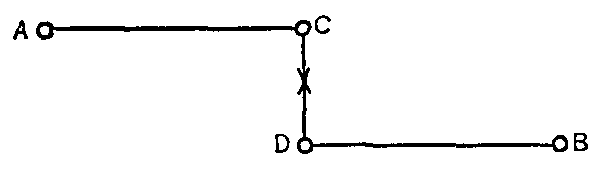
\includegraphics[width=50mm]{images/JJSfig1.png}
\end{center}

Euclid bases his \emph{Elements} on two postulates; first, that a
straight line can be drawn, second, that a circle can be
described. It is sometimes expressed in this way; he postulates a
ruler and compass. The latter contrivance is not difficult to
construct, because it does not involve the use of a ruler or a
compass in its own construction. But how is a ruler to be made
straight, unless you already have a ruler by which to test it? The
problem is to devise a mechanism which shall assume the second
postulate only, and be able to satisfy the first. It is the
mechanical problem of converting motion in a circle into motion in
a straight line, without the use of any guide. James Watt, the
inventor of the steam-engine, tackled the problem with all his
might, but gave it up as impossible. However, he succeeded in
finding a contrivance which solves the problem very approximately.
Watt's parallelogram, employed in nearly every beam-engine,
consists of three links; of which \emph{AC} and \emph{BD} are
equal, and have fixed pivots at \emph{A} and \emph{B}
respectively. The link \emph{CD} is of such a length that
\emph{AC} and \emph{BD} are parallel when horizontal. The tracing
point is attached to the middle point of \emph{CD}. When \emph{C}
and \emph{D} move round their pivots, the tracing point describes
a straight line very approximately, so long as the arc of
displacement is small. The complete figure which would be
described is the figure of 8, and the part utilized is near the
point of contrary flexure.

\begin{center}
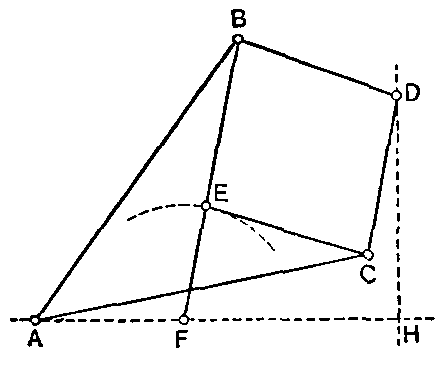
\includegraphics[width=50mm]{images/JJSfig2.png}
\end{center}

A linkage giving a closer approximation to a straight line was
also invented by the Russian mathematician before
mentioned---Tschebicheff; it likewise made use of three links. But
the linkage invented by Peaucellier and later by Lipkin had seven
pieces. The arms \emph{AB} and \emph{AC} are of equal length, and
have a fixed pivot at \emph{A}. The links \emph{DB}, \emph{BE},
\emph{EC}, \emph{CD} are of equal length. \emph{EF} is an arm
connecting \emph{E} with the fixed pivot \emph{F} and is equal in
length to the distance between \emph{A} and \emph{F}. It is
readily shown by geometry that, as the point \emph{E} describes a
circle around the center \emph{F}, the point \emph{D} describes an
exact straight line perpendicular to the line joining it and
\emph{F}. The exhibition of this contrivance at work was the
climax of Sylvester's lecture.

In Sylvester's audience were two mathematicians, Hart and Kempe,
who took up the subject for further investigation. Hart perceived
that the contrivances of Watt and of Tschebicheff consisted of
three links, whereas Peaucellier's consisted of seven. Accordingly
he searched for a contrivance of five links which would enable a
tracing point to describe a perfect straight line; and he
succeeded in inventing it. Kempe was a London barrister whose
specialty was ecclesiastical law. He and Sylvester worked up the
theory of linkages together, and discovered among other things the
skew pantograph. Kempe became so imbued with linkage that he
contributed to the Royal Society of London a paper on the ``Theory
of Mathematical Form,'' in which he explains all reasoning by
means of linkages.

About this time (1877) the Johns Hopkins University was organized
at Baltimore, and Sylvester, at the age of 63, was appointed the
first professor of mathematics. Of his work there as a teacher,
one of his pupils, Dr.\ Fabian Franklin, thus spoke in an address
delivered at a memorial meeting in that University: ``The one
thing which constantly marked Sylvester's lectures was
enthusiastic love of the thing he was doing. He had in the fullest
possible degree, to use the French phrase, the defect of this
quality; for as he almost always spoke with enthusiastic ardor, so
it was almost never possible for him to speak on matters incapable
of evoking this ardor. In other words, the substance of his
lectures had to consist largely of his own work, and, as a rule,
of work hot from the forge. The consequence was that a continuous
and systematic presentation of any extensive body of doctrine
already completed was not to be expected from him. Any unsolved
difficulty, any suggested extension, such as would have been
passed by with a mention by other lecturers, became inevitably
with him the occasion of a digression which was sure to consume
many weeks, if indeed it did not take him away from the original
object permanently. Nearly all of the important memoirs which he
published, while in Baltimore, arose in this way. We who attended
his lectures may be said to have seen these memoirs in the making.
He would give us on the Friday the outcome of his grapplings with
the enemy since the Tuesday lecture. Rarely can it have fallen to
the lot of any class to follow so completely the workings of the
mind of the master. Not only were all thus privileged to see `the
very pulse of the machine,' to learn the spring and motive of the
successive steps that led to his results, but we were set aglow by
the delight and admiration which, with perfect na\"{\i}vet\'e and
with that luxuriance of language peculiar to him, Sylvester
lavished upon these results. That in this enthusiastic admiration
he sometimes lacked the sense of proportion cannot be denied. A
result announced at one lecture and hailed with loud acclaim as a
marvel of beauty was by no means sure of not being found before
the next lecture to have been erroneous; but the Esther that
supplanted this Vashti was quite certain to be found still more
supremely beautiful. The fundamental thing, however, was not this
occasional extravagance, but the deep and abiding feeling for
truth and beauty which underlay it. No young man of generous mind
could stand before that superb grey head and hear those
expositions of high and dear-bought truths, testifying to a
passionate devotion undimmed by years or by arduous labors,
without carrying away that which ever after must give to the
pursuit of truth a new and deeper significance in his mind.''

One of Sylvester's principal achievements at Baltimore was the
founding of the \emph{American Journal of Mathematics}, which, at
his suggestion, took the quarto form. He aimed at establishing a
mathematical journal in the English language, which should equal
Liouville's \emph{Journal} in France, or Crelle's \emph{Journal}
in Germany. Probably his best contribution to the \emph{American
Journal} consisted in his ``Lectures on Universal Algebra'';
which, however, were left unfinished, like a great many other
projects of his.

Sylvester had that quality of absent-mindedness which is popularly
supposed to be, if not the essence, at least an invariable
accompaniment, of a distinguished mathematician. Many stories are
related on this point, which, if not all true, are at least
characteristic. Dr.\ Franklin describes an instance which actually
happened in Baltimore. To illustrate a theory of versification
contained in his book \emph{The Laws of Verse}, Sylvester prepared
a poem of 400 lines, all rhyming with the name Rosal\u\i{}nd or
Rosal\=\i{}nd; and it was announced that the professor would read
the poem on a specified evening at a specified hour at the Peabody
Institute. At the time appointed there was a large turn-out of
ladies and gentlemen. Prof.\ Sylvester, as usual, had a number of
footnotes appended to his production; and he announced that in
order to save interruption in reading the poem itself, he would
first read the footnotes. The reading of the footnotes suggested
various digressions to his imagination; an hour had passed, still
no poem; an hour and a half passed and the striking of the clock
or the unrest of his audience reminded him of the promised poem.
He was astonished to find how time had passed, excused all who had
engagements, and proceeded to read the Rosalind poem.

In the summer of 1881 I visited London to see the Electrical
Exhibition in the Crystal Palace---one of the earliest exhibitions
devoted to electricity exclusively. I had made some investigations
on the electric discharge, using a Holtz machine where De LaRue
used a large battery of cells. Mr.\ De LaRue was Secretary of the
Royal Institution; he gave me a ticket to a Friday evening
discourse to be delivered by Mr.\ Spottiswoode, then president of
the Royal Society, on the phenomena of the intensive discharge of
electricity through gases; also an invitation to a dinner at his
own house to be given prior to the lecture. Mr.\ Spottiswoode, the
lecturer for the evening, was there; also Prof.\ Sylvester. He was
a man rather under the average height, with long gray beard and a
profusion of gray locks round his head surmounted by a great dome
of forehead. He struck me as having the appearance of an artist or
a poet rather than of an exact scientist. After dinner he
conversed very eloquently with an elderly lady of title, while I
conversed with her daughter. Then cabs were announced to take us
to the Institution. Prof.\ Sylvester and I, being both bachelors,
were put in a cab together. The professor, who had been so
eloquent with the lady, said nothing; so I asked him how he liked
his work at the Johns Hopkins University. ``It is very pleasant
work indeed,'' said he, ``and the young men who study there are
all so enthusiastic.'' We had not exhausted that subject before we
reached our destination. We went up the stairway together, then
Sylvester dived into the library to see the last number of
\emph{Comptes Rendus} (in which he published many of his results
at that time) and I saw him no more. I have always thought it very
doubtful whether he came out to hear Spottiswoode's lecture.

We have seen that H.~J.~S.\ Smith, the Savilian professor of
Geometry at Oxford, died in 1883. Sylvester's friends urged his
appointment, with the result that he was elected. After two years
he delivered his inaugural lecture; of which the subject was
differential invariants, termed by him reciprocants. An elementary
reciprocant is $\frac{d^{2}y}{dx^{2}}$, for if
$\frac{d^{2}y}{dx^{2}}=0$ then $\frac{d^{2}x}{dy^{2}}=0$. He
looked upon this as the ``grub'' form, and developed from it the
``chrysalis''
\begin{equation*}
\left\vert
\begin{array}{ccc}
\frac{d^{2}\phi}{dx^{2}}&\frac{d^{2}\phi}{dxdy}&\frac{d\phi}{dx},\\
\frac{d^{2}\phi}{dxdy}&\frac{d^{2}\phi}{dy^{2}}&\frac{d\phi}{dy},\\
\frac{d\phi}{dx}&\frac{d\phi}{dy}&\cdot
\end{array}
\right\vert
\end{equation*}
\noindent and the ``imago''
\begin{equation*}
\left\vert
\begin{array}{ccc}
\frac{d^{2}\Phi}{dx^{2}}&\frac{d^{2}\Phi}{dxdy}&\frac{d^{2}\Phi}{dxdr},\\
\frac{d^{2}\Phi}{dxdy}&\frac{d^{2}\Phi}{dy^{2}}&\frac{d^{2}\Phi}{dydr},\\
\frac{d^{2}\Phi}{dxdr}&\frac{d^{2}\Phi}{dydr}&\frac{d^{2}\Phi}{dr^{2}}.
\end{array}
\right\vert
\end{equation*}
\noindent You will observe that the chrysalis expression is
unsymmetrical; the place of a ninth term is vacant. It moved
Sylvester's poetic imagination, and into his inaugural lecture he
interjected the following sonnet:

\begin{center}
\textsc{To a Missing Member of a Family Group of Terms in an
Algebraical Formula:}
\end{center}

\begin{verse}
Lone and discarded one! divorced by fate, \\
Far from thy wished-for fellows---whither art flown? \\
Where lingerest thou in thy bereaved estate, \\
Like some lost star, or buried meteor stone? \\
Thou minds't me much of that presumptuous one, \\
Who loth, aught less than greatest, to be great, \\
From Heaven's immensity fell headlong down \\
To live forlorn, self-centred, desolate: \\
Or who, new Heraklid, hard exile bore, \\
Now buoyed by hope, now stretched on rack of fear, \\
Till throned Astr\ae{}a, wafting to his ear \\
Words of dim portent through the Atlantic roar, \\
Bade him ``the sanctuary of the Muse revere \\
And strew with flame the dust of Isis' shore.''
\end{verse}

This inaugural lecture was the beginning of his last great
contribution to mathematics, and the subsequent lectures of that
year were devoted to his researches in that line. Smith and
Sylvester were akin in devoting attention to the theory of
numbers, and also in being eloquent speakers. But in other
respects the Oxonians found a great difference. Smith had been a
painstaking tutor; Sylvester could lecture only on his own
researches, which were not popular in a place so wholly given over
to examinations. Smith was an incessantly active man of affairs;
Sylvester became the subject of melancholy and complained that he
had no friends.

In 1872 a deputy professor was appointed. Sylvester removed to
London, and lived mostly at the Athen\ae{}um Club. He was now 78
years of age, and suffered from partial loss of sight and memory.
He was subject to melancholy, and his condition was indeed
``forlorn and desolate.'' His nearest relatives were nieces, but
he did not wish to ask their assistance. One day, meeting a
mathematical friend who had a home in London, he complained of the
fare at the Club, and asked his friend to help him find suitable
private apartments where he could have better cooking. They drove
about from place to place for a whole afternoon, but none suited
Sylvester. It grew late: Sylvester said, ``You have a pleasant
home: take me there,'' and this was done. Arrived, he appointed
one daughter his reader and another daughter his amanuensis.
``Now,'' said he, ``I feel comfortably installed; don't let my
relatives know where I am.'' The fire of his temper had not dimmed
with age, and it required all the Christian fortitude of the
ladies to stand his exactions. Eventually, notice had to be sent
to his nieces to come and take charge of him. He died on the 15th
of March, 1897, in the 83d year of his age, and was buried in the
Jewish cemetery at Dalston.

As a theist, Sylvester did not approve of the destructive attitude
of such men as Clifford, in matters of religion. In the early days
of his career he suffered much from the disabilities attached to
his faith, and they were the prime cause of so much ``fighting the
world.'' He was, in all probability, a greater mathematical genius
than Cayley; but the environment in which he lived for some years
was so much less favorable that he was not able to accomplish an
equal amount of solid work. Sylvester's portrait adorns St.\
John's College, Cambridge. A memorial fund of \pounds1500 has been
placed in the charge of the Royal Society of London, from the
proceeds of which a medal and about \pounds100 in money is awarded
triennially for work done in pure mathematics. The first award has
been made to M.\ Henri Poincar\'e of Paris, a mathematician for
whom Sylvester had a high professional and personal regard.

\chapter [Thomas Penyngton Kirkman (1806-1895)]{THOMAS \\
PENYNGTON KIRKMAN\footnote{This Lecture was delivered April 20,
1903.---\textsc{Editors.}}}

\large\begin{center}{(1806-1895)}\end{center}\normalsize

Thomas Penyngton Kirkman was born on March 31, 1806, at Bolton in
Lancashire. He was the son of John Kirkman, a dealer in cotton and
cotton waste; he had several sisters but no brother. He was
educated at the Grammar School of Bolton, where the tuition was
free. There he received good instruction in Latin and Greek, but
no instruction in geometry or algebra; even Arithmetic was not
then taught in the headmaster's upper room. He showed a decided
taste for study and was by far the best scholar in the school. His
father, who had no taste for learning and was succeeding in trade,
was determined that his only son should follow his own business,
and that without any loss of time. The schoolmaster tried to
persuade the father to let his son remain at school; and the vicar
also urged the father, saying that if he would send his son to
Cambridge University, he would guarantee for sixpence that the boy
would win a fellowship. But the father was obdurate; young Kirkman
was removed from school, when he was fourteen years of age, and
placed at a desk in his father's office. While so engaged, he
continued of his own accord his study of Latin and Greek, and
added French and German.

After ten years spent in the counting room, he tore away from his
father, secured the tuition of a young Irish baronet, Sir John
Blunden, and entered the University of Dublin with the view of
passing the examinations for the degree of B.A. There he never had
instruction from any tutor. It was not until he entered Trinity
College, Dublin, that he opened any mathematical book. He was not
of course abreast with men who had good preparation. What he knew
of mathematics, he owed to his own study, having never had a
single hour's instruction from any person. To this self-education
is due, it appears to me, both the strength and the weakness to be
found in his career as a scientist. However, in his college course
he obtained honors, or premiums as they are called, and graduated
as a moderator, something like a wrangler.

Returning to England in 1835, when he was 29 years old, he was
ordained as a minister in the Church of England. He was a curate
for five years, first at Bury, afterwards at Lymm; then he became
the vicar of a newly-formed parish---Croft with Southworth in
Lancashire. This parish was the scene of his life's labors. The
income of the benefice was not large, about \pounds200 per annum;
for several years he supplemented this by taking pupils. He
married, and property which came to his wife enabled them to
dispense with the taking of pupils. His father became poorer, but
was able to leave some property to his son and daughters. His
parochial work, though small, was discharged with enthusiasm; out
of the roughest material he formed a parish choir of boys and
girls who could sing at sight any four-part song put before them.
After the private teaching was over he had the leisure requisite
for the great mathematical researches in which he now engaged.

Soon after Kirkman was settled at Croft, Sir William Rowan
Hamilton began to publish his quaternion papers and, being a
graduate of Dublin University, Kirkman was naturally one of the
first to study the new analysis. As the fruit of his meditations
he contributed a paper to the \emph{Philosophical Magazine} ``On
pluquaternions and homoid products of sums of \emph{n} squares.''
He proposed the appellation "pluquaternions" for a linear
expression involving more than three imaginaries (the $i$, $j$,
$k$ of Hamilton), ``not dreading'' he says, ``the pluperfect
criticism of grammarians, since the convenient barbarism is their
own.'' Hamilton, writing to De~Morgan, remarked ``Kirkman is a
very clever fellow,'' where the adjective has not the American
colloquial meaning but the English meaning.

For his own education and that of his pupils he devoted much
attention to mathematical mnemonics, studying the \emph{Memoria
Technica} of Grey. In 1851 he contributed a paper on the subject
to the Literary and Philosophical Society of Manchester, and in
1852 he published a book, \emph{First Mnemonical Lessons in
Geometry, Algebra, and Trigonometry}, which is dedicated to his
former pupil, Sir John Blunden. De~Morgan pronounced it ``the most
curious crochet I ever saw,'' which was saying a great deal, for
De~Morgan was familiar with many quaint books in mathematics. In
the preface he says that much of the distaste for mathematical
study springs largely from the difficulty of retaining in the
memory the previous results and reasoning. ``This difficulty is
closely connected with the unpronounceableness of the formul\ae{};
the memory of the tongue and the ear are not easily turned to
account; nearly everything depends on the thinking faculty or on
the practice of the eye alone. Hence many, who see hardly anything
formidable in the study of a language, look upon mathematical
acquirements as beyond their power, when in truth they are very
far from being so. My object is to enable the learner to `talk to
himself,' in rapid, vigorous and suggestive syllables, about the
matters which he must digest and remember. I have sought to bring
the memory of the vocal organs and the ear to the assistance of
the reasoning faculty and have never scrupled to sacrifice either
good grammar or good English in order to secure the requisites for
a useful \emph{mnemonic}, which are smoothness, condensation, and
jingle.''

As a specimen of his mnemonics we may take the cotangent formula
in spherical trigonometry:

\begin{equation*}
\cot A \sin C + \cos b \cos C = \cot a \sin b
\end{equation*}

To remember this formula most masters then required some aid to
the memory; for instance the following: If in any spherical
triangle four parts be taken in succession, such as \emph{AbCa},
consisting of two means \emph{bC} and two extremes \emph{Aa}, then
the product of the cosines of the two means is equal to the sine
of the mean side $\times$ cotangent of the extreme side minus sine
of the mean angle $\times$ cotangent of the extreme angle, that is

\begin{equation*}
\cos b \cos C = \sin b \cot a - \sin C \cot A.
\end{equation*}

This is an appeal to the reason. Kirkman, however, proceeds on the
principle of appealing to the memory of the ear, of the tongue,
and of the lips altogether; a true \emph{memoria technica}. He
distinguishes the large letter from the small by calling them
\emph{Ang, Bang, Cang} (\emph{ang} from angle in contrast to
side). To make the formula more euphoneous he drops the s from cos
and the n from sin. Hence the formula is
\medskip
\begin{center}
cot \emph{Ang} si \emph{Cang} and co \emph{b} co \emph{Cang} are
cot \emph{a} si \emph{b}
\end{center}
\medskip
\noindent which is to be chanted till it becomes perfectly
familiar to the ear and the lips. The former rule is a hint
offered to the judgment; Kirkman's method is something to be
taught by rote. In his book Kirkman makes much use of verse, in
the turning of which he was very skillful.

In the early part of the nineteenth century a publication named
the \emph{Lady's and Gentlemen's Diary} devoted several columns to
mathematical problems. In 1844 the editor offered a prize for the
solution of the following question: ``Determine the number of
combinations that can be made out of $n$ symbols, each combination
having $p$ symbols, with this limitation, that no combination of
$q$ symbols which may appear in any one of them, may be repeated
in any other.'' This is a problem of great difficulty; Kirkman
solved it completely for the special case of $p=3$ and $q=2$ and
printed his results in the second volume of the \emph{Cambridge
and Dublin Mathematical Journal}. As a chip off this work he
published in the \emph{Diary} for 1850 the famous problem of the
fifteen schoolgirls as follows: ``Fifteen young ladies of a school
walk out three abreast for seven days in succession; it is
required to arrange them daily so that no two shall walk abreast
more than once.'' To form the schedules for seven days is not
difficult; but to find all the possible schedules is a different
matter. Kirkman found all the possible combinations of the fifteen
young ladies in groups of three to be 35, and the problem was also
considered and solved by Cayley, and has been discussed by many
later writers; Sylvester gave 91 as the greatest number of days;
and he also intimated that the principle of the puzzle was known
to him when an undergraduate at Cambridge, and that he had given
it to fellow undergraduates. Kirkman replied that up to the time
he proposed the problem he had neither seen Cambridge nor met
Sylvester, and narrated how he had hit on the question.

The Institute of France offered several times in succession a
prize for a memoir on the theory of the polyedra; this fact
together with his work in combinations led Kirkman to take up the
subject. He always writes \emph{polyedron} not \emph{polyhedron};
for he says we write \emph{periodic} not \emph{perihodic}. When
Kirkman began work nothing had been done beyond the very ancient
enumeration of the five regular solids and the simple combinations
of crystallography. His first paper, ``On the representation and
enumeration of the polyedra,'' was communicated in 1850 to the
Literary and Philosophical Society of Manchester. He starts with
the well-known theorem $P+S = L+2$, where $P$ is the number of
points or summits, $S$ the number of plane bounding surfaces and
$L$ the number of linear edges in a geometrical solid. "The
question---how many $n$-edrons are there?---has been asked, but it
is not likely soon to receive a definite answer. It is far from
being a simple question, even when reduced to the narrower
compass---how many $n$-edrons are there whose summits are all
trihedral"? He enumerated and constructed the fourteen 8-edra
whose faces are all triangles.

In 1858 the French Institute modified its prize question. As the
subject for the \emph{concours} of 1861 was announced:
``Perfectionner en quelque point important la th\'eorie
g\'eom\'etrique des poly\`edres,'' where the indefiniteness of the
question indicates the very imperfect state of knowledge on the
subject. The prize offered was 3000 francs. Kirkman appears to
have worked at it with a view of competing, but he did not send in
his memoir. Cayley appears to have intended to compete. The time
was prolonged for a year, but there was no award and the prize was
taken down. Kirkman communicated his results to the Royal Society
through his friend Cayley, and was soon elected a Fellow. Then he
contributed directly an elaborate paper entitled ``Complete theory
of the Polyedra.'' In the preface he says, ``The following memoir
contains a complete solution of the classification and enumeration
of the $P$-edra $Q$-acra. The actual construction of the solids is
a task impracticable from its magnitude, but it is here shown that
we can enumerate them with an accurate account of their symmetry
to any values of \emph{P} and \emph{Q}.'' The memoir consisted of
21 sections; only the two introductory sections, occupying 45
quarto pages, were printed by the Society, while the others still
remain in manuscript. During following years he added many
contributions to this subject.

In 1858 the French Academy also proposed a problem in the Theory
of Groups as the subject for competition for the grand
mathematical prize in 1860: ``Quels peuvent \^etre les nombres de
valeurs des fonctions bien d\'efinies qui contiennent un nombre
donn\'e de lettres, et comment peut on former les fonctions pour
lesquelles il existe un nombre donn\'e de valeurs?'' Three memoirs
were presented, of which Kirkman's was one, but no prize was
awarded. Not the slightest summary was vouchsafed of what the
competitors had added to science, although it was confessed that
all had contributed results both new and important; and the
question, though proposed for the first time for the year 1860,
was withdrawn from competition contrary to the usual custom of the
Academy. Kirkman contributed the results of his investigation to
the Manchester Society under the title ``The complete theory of
groups, being the solution of the mathematical prize question of
the French Academy for 1860.'' In more recent years the theory of
groups has engaged the attention of many mathematicians in Germany
and America; so far as British contributors are concerned Kirkman
was the first and still remains the greatest.

In 1861 the British Association met at Manchester; it was the last
of its meetings which Sir William Rowan Hamilton attended. After
the meeting Hamilton visited Kirkman at his home in the Croft
rectory, and that meeting was no doubt a stimulus to both. As
regards pure mathematics they were probably the two greatest in
Britain; both felt the loneliness of scientific work, both were
metaphysicians of penetrating power, both were good versifiers if
not great poets. Of nearly the same age, they were both endowed
with splendid physique; but the care which was taken of their
health was very different; in four years Hamilton died but Kirkman
lived more than 30 years longer.

About 1862 the \emph{Educational Times}, a monthly periodical
published in London, began to devote several columns to the
proposing and solving of mathematical problems, taking up the work
after the demise of the \emph{Diary}. This matter was afterwards
reprinted in separate volumes, two for each year. In these
reprints are to be found many questions proposed by Kirkman; they
are generally propounded in quaint verse, and many of them were
suggested by his study of combinations. A good specimen is ``The
Revenge of Old King Cole''

\begin{verse}
``Full oft ye have had your fiddler's fling, \\
For your own fun over the wine; \\
And now'' quoth Cole, the merry old king, \\
``Ye shall have it again for mine. \\
My realm prepares for a week of joy \\
At the coming of age of a princely boy--- \\
Of the grand six days procession in square, \\
In all your splendour dressed, \\
Filling the city with music rare \\
From fiddlers five abreast,'' etc.
\end{verse}

The problem set forth by this and other verses is that of 25 men
arranged in five rows on Monday. Shifting the second column one
step upward, the third two steps, the fourth three steps, and the
fifth four steps gives the arrangement for Tuesday. Applying the
same rule to Tuesday gives Wednesday's array, and similarly are
found those for Thursday and Friday. In none of these can the same
two men be found in one row. But the rule fails to work for
Saturday, so that a special arrangement must be brought in which I
leave to my hearers to work out. This problem resembles that of
the fifteen schoolgirls.

\begin{center}
\begin{tabular}{ccccc}
\multicolumn{5}{c}{Monday} \\
A&B&C&D&E \\
F&G&H&I&J \\
K&L&M&N&O \\
P&Q&R&S&T \\
U&V&W&X&Y
\end{tabular} \hspace{10 mm}
\begin{tabular}{ccccc}
\multicolumn{5}{c}{Tuesday} \\
A&G&M&S&Y \\
F&L&R&X&E \\
K&Q&W&D&J \\
P&V&C&I&O \\
U&B&H&N&T
\end{tabular}

\medskip
\begin{tabular}{ccccc}
\multicolumn{5}{c}{Wednesday} \\
A&L&W&I&T \\
F&Q&C&N&Y \\
K&V&H&S&E \\
P&B&M&X&J \\
N&G&R&D&O
\end{tabular} \hspace{10 mm}
\begin{tabular}{ccccc}
\multicolumn{5}{c}{Thursday} \\
A&Q&H&X&O \\
F&V&M&D&T \\
K&B&R&I&Y \\
P&G&W&N&E \\
U&L&C&S&J
\end{tabular}
\end{center}

The Rev.\ Kirkman became at an early period of his life a broad
churchman. About 1863 he came forward in defense of the Bishop of
Colenso, a mathematician, and later he contributed to a series of
pamphlets published in aid of the cause of ``Free Enquiry and Free
Expression.'' In one of his letters to me Kirkman writes as
follows: ``\emph{The Life of Colenso} by my friend Rev.\ Sir
George Cox, Bart., is a most charming book; and the battle of the
Bishops against the lawyers in the matter of the vacant see of
Natal, to which Cox is the bishop-elect, is exciting. Canterbury
refuses to ask, as required, the Queen's mandate to consecrate
him. The Natal churchmen have just petitioned the Queen to make
the Primate do his duty according to law. Natal was made a See
with perpetual succession, and is endowed. The endowment has been
lying idle since Colenso's death in 1883; and the bishops who have
the law courts dead against them here are determined that no
successor to Colenso shall be consecrated. There is a Bishop of
South African Church there, whom they thrust in while Colenso
lived, on pretense that Colenso was excommunicate. We shall soon
see whether the lawyers or the bishops are to win.'' It was
Kirkman's own belief that his course in this matter injured his
chance of preferment in the church; he never rose above being
rector of Croft.

While a broad churchman the Rev.\ Mr.\ Kirkman was very vehement
against the leaders of the materialistic philosophy. Two years
after Tyndall's Belfast address, in which he announced that he
could discern in matter the promise and potency of every form of
life, Kirkman published a volume entitled \emph{Philosophy without
Assumptions}, in which he criticises in very vigorous style the
materialistic and evolutional philosophy advocated by Mill,
Spencer, Tyndall, and Huxley. In ascribing everything to matter
and its powers or potencies he considers that they turn philosophy
upside down. He has, he writes, first-hand knowledge of himself as
a continuous person, endowed with will; and he infers that there
are will forces around; but he sees no evidence of the existence
of matter. Matter is an assumption and forms no part of his
philosophy. He relies on Boscovich's theory of an atom as simply
the center of forces. Force he understands from his knowledge of
will, but any other substance he does not understand. The obvious
difficulty in this philosophy is to explain the belief in the
existence of other conscious beings---other will forces. Is it not
the \emph{great} assumption which everyone is obliged to make;
verified by experience, but still in its nature an assumption?
Kirkman tries to get over this difficulty by means of a syllogism,
the major premise of which he has to manufacture, and which he
presents to his reason for adoption or rejection. How can a
universal proposition be easier to grasp than the particular case
included in it?  If the mind doubts about an individual case, how
can it be sure about an infinite number of such cases? It is a
\emph{petitio principii}.

As a critic of the materialistic philosophy Kirkman is more
successful. He criticises Herbert Spencer on free will as follows:
``The short chapter of eight pages on Will cost more philosophical
toil than all the two volumes on Psychology. The author gets
himself in a heat, he runs himself into a corner, and brings
himself dangerously to bay. Hear him: `To reduce the general
question to its simplest form; psychical changes either conform to
law, or they do not. If they do not conform to law, this work, in
common with all other works on the subject, is sheer nonsense;  no
science of Psychology is possible. If they do conform to law,
there cannot be any such thing as free will.' Here we see the
horrible alternative. If the assertors of free will refuse to
commit suicide, they must endure the infinitely greater pang of
seeing Mr.\ Spencer hurl himself and his books into that yawning
gulf, a sacrifice long devoted, and now by pitiless Fate
consigned, to the abysmal gods of nonsense. Then pitch him down
say I. Shall I spare him who tells me that my movements in this
orbit of conscious thought and responsibility are made under
`parallel conditions' with those of yon driven moon? Shall I spare
him who has juggled me out of my Will, my noblest attribute; who
has hocuspocused me out of my subsisting personality; and then, as
a refinement of cruelty, has frightened me out of the rest of my
wits by forcing me to this terrific alternative that either the
testimony of this Being, this Reason and this Conscience is one
ever-thundering lie, or else he, even he, has talked nonsense? He
has talked nonsense, I say it because I have proved it. And every
man must of course talk nonsense who begins his philosophy with
abstracts in the clouds instead of building on the witness of his
own self-consciousness. `If they do conform to law,' says Spencer,
`there cannot be any such thing as free will.' The force of this
seems to depend on his knowledge of `law.' When I ask, What does
this writer know of law---definite working law in the
Cosmos?---the only answer I can get is---Nothing, except a very
little which he has picked up, often malappropriately, as we have
seen, among the mathematicians. When I ask---What does he know
\emph{about} law?---there is neither beginning nor end to the
reply. I am advised to read his books \emph{about} law, and to
master the differentiations and integrations of the coherences,
the correlations, the uniformities, and universalities which he
has established in the abstract over all space and all time by his
vast experience and miraculous penetration. I have tried to do
this, and have found all pretty satisfactory, except the lack of
one thing---something like proof of his competence to decide all
that scientifically. When I persist in my demand for such proof,
it turns out at last---that he knows by heart the whole Hymn Book,
the Litanies, the Missal, and the Decretals of the Must-be-ite
religion! `Conform to law.' Shall I tell you what he means by
that? Exactly ninety-nine hundredths of his meaning under the word
\emph{law} is \emph{must be}.''

Kirkman points out that the kind of proof offered by these
philosophers is a bold assertion of \emph{must-be-so}. For
instance he mentions Spencer's evolution of consciousness out of
the unconscious: ``That an effectual adjustment may be made they
(the separate impressions or constituent changes of a complex
correspondence to be coordinated) \emph{must be} brought into
relation with each other. But this implies some center of
communication common to them all, through which they severally
pass; and as they \emph{cannot} pass through it simultaneously,
they \emph{must} pass through it in succession. So that as the
external phenomena responded to become greater in number and more
complicated in kind, the variety and rapidity of the changes to
which this common center of communication is subject \emph{must}
increase, there \emph{must} result an unbroken series of those
changes, there \emph{must} arise a consciousness.''

The paraphrase which Kirkman gave of Spencer's definition of
Evolution commended itself to such great minds as Tait and
Clerk-Maxwell. Spencer's definition is: ``Evolution is a change
from an indefinite incoherent homogeneity to a definite coherent
heterogeneity, through continuous differentiations and
integrations.'' Kirkman's paraphrase is ``Evolution is a change
from a nohowish untalkaboutable all-likeness, to a somehowish and
in-general-talkaboutable not-all-likeness, by continuous
somethingelseifications and sticktogetherations.'' The tone of
Kirkman's book is distinctly polemical and full of sarcasm. He
unfortunately wrote as a theologian rather than as a
mathematician. The writers criticised did not reply, although they
felt the edge of his sarcasm; and they acted wisely, for they
could not successfully debate any subject involving exact science
against one of the most penetrating mathematicians of the
nineteenth century.

We have seen that Hamilton appreciated Kirkman's genius; so did
Cayley, De~Morgan, Clerk-Maxwell, Tait. One of Tait's most
elaborate researches was the enumeration and construction of the
knots which can be formed in an endless cord---a subject which he
was induced to take up on account of its bearing on the vortex
theory of atoms. If the atoms are vortex filaments their
differences in kind, giving rise to differences in the spectra of
the elements, must depend on a greater or less complexity in the
form of the closed filament, and this difference would depend on
the knottiness of the filament. Hence the main question was ``How
many different forms of knots are there with any given small
number of crossings?'' Tait made the investigation for three,
four, five, six, seven, eight crossings. Kirkman's investigations
on the polyedra were much allied. He took up the problem and, with
some assistance from Tait, solved it not only for nine but for ten
crossings. An investigation by C.~N.\ Little, a graduate of Yale
University, has confirmed Kirkman's results.

Through Professor Tait I was introduced to Rev.\ Mr.\ Kirkman; and
we discussed the mathematical analysis of relationships, formal
logic, and other subjects. After I had gone to the University of
Texas, Kirkman sent me through Tait the following question which
he said was current in society: ``Two boys, Smith and Jones, of
the same age, are each the nephew of the other; how many legal
solutions?'' I set the analysis to work, wrote out the solutions,
and the paper is printed in the \emph{Proceedings} of the Royal
Society of Edinburgh. There are four solutions, provided Smith and
Jones are taken to be mere arbitrary, names; if the convention
about surnames holds there are only two legal solutions. On seeing
my paper Kirkman sent the question to the \emph{Educational Times}
in the following improved form:

\begin{verse}
Baby Tom of baby Hugh \\
The nephew is and uncle too; \\
In how many ways can this be true?
\end{verse}

Thomas Penyngton Kirkman died on February 3, 1895, having very
nearly reached the age of 89 years. I have found only one printed
notice of his career, but all his writings are mentioned in the
new German Encyclop\ae{}dia of Mathematics. He was an honorary
member of the Literary and Philosophical Societies of Manchester
and of Liverpool, a Fellow of the Royal Society, and a foreign
member of the Dutch Society of Sciences at Haarlem. I may close by
a quotation from one of his letters: ``What I have done in helping
busy Tait in knots is, like the much more difficult and extensive
things I have done in polyedra or groups, not at likely to be
talked about intelligently by people so long as I live. But it is
a faint pleasure to think it will one day win a little praise.''


\chapter [Isaac Todhunter (1820-1884)]{ISAAC
TODHUNTER\footnote{This Lecture was delivered April 13,
1904.---\textsc{Editors.}}}

\large\begin{center}{(1820-1884)}\end{center}\normalsize

Isaac Todhunter was born at Rye, Sussex, 23 Nov., 1820. He was the
second son of George Todhunter, Congregationalist minister of the
place, and of Mary his wife, whose maiden name was Hume, a
Scottish surname. The minister died of consumption when Isaac was
six years old, and left his family, consisting of wife and four
boys, in narrow circumstances. The widow, who was a woman of
strength, physically and mentally, moved to the larger town of
Hastings in the same county, and opened a school for girls. After
some years Isaac was sent to a boys' school in the same town kept
by Robert Carr, and subsequently to one newly opened by a Mr.\
Austin from London; for some years he had been unusually backward
in his studies, but under this new teacher he made rapid progress,
and his career was then largely determined.

After his school days were over, he became an usher or assistant
master with Mr.\ Austin in a school at Peckham; and contrived to
attend at the same time the evening classes at University College,
London. There he came under the great educating influence of
De~Morgan, for whom in after years he always expressed an
unbounded admiration; to De~Morgan ``he owed that interest in the
history and bibliography of science, in moral philosophy and logic
which determined the course of his riper studies.'' In 1839 he
passed the matriculation examination of the University of London,
then a merely examining body, winning the exhibition for
mathematics (\pounds30 for two years); in 1842 he passed the B.A.\
examination carrying off a mathematical scholarship (of \pounds50
for three years); and in 1844 obtained the degree of Master of
Arts with the gold medal awarded to the candidate who gained the
greatest distinction in that examination.

Sylvester was then professor of natural philosophy in University
College, and Todhunter studied under him. The writings of Sir John
Herschel also had an influence; for Todhunter wrote as follows
(\emph{Conflict of Studies}, p.\ 66): ``Let me at the outset
record my opinion of mathematics; I cannot do this better than by
adopting the words of Sir J.\ Herschel, to the influence of which
I gratefully attribute the direction of my own early studies. He
says of Astronomy, `Admission to its sanctuary can only be gained
by one means,---sound and sufficient knowledge of mathematics, the
great instrument of all exact inquiry, without which no man can
ever make such advances in this or any other of the higher
departments of science as can entitle him to form an independent
opinion on any subject of discussion within their range.'\,''

When Todhunter graduated as M.A.\ he was 24 years of age.
Sylvester had gone to Virginia, but De~Morgan remained. The latter
advised him to go through the regular course at Cambridge; his
name was now entered at St.\ John's College. Being somewhat older,
and much more brilliant than the honor men of his year, he was
able to devote a great part of his attention to studies beyond
those prescribed. Among other subjects he took up Mathematical
Electricity. In 1848 he took his B.A.\ degree as senior wrangler,
and also won the first Smith's prize.

While an undergraduate Todhunter lived a very secluded life. He
contributed along with his brothers to the support of their
mother, and he had neither money nor time to spend on
entertainments. The following legend was applied to him, if not
recorded of him: ``Once on a time, a senior wrangler gave a wine
party to celebrate his triumph. Six guests took their seats round
the table. Turning the key in the door, he placed one bottle of
wine on the table asseverating with unction, `None of you will
leave this room while a single drop remains.'\,''

At the University of Cambridge there is a foundation which
provides for what is called the Burney prize. According to the
regulations the prize is to be awarded to a graduate of the
University who is not of more than three years' standing from
admission to his degree and who shall produce the best English
essay ``On some moral or metaphysical subject, or on the
existence, nature and attributes of God, or on the truth and
evidence of the Christian religion.'' Todhunter in the course of
his first postgraduate year submitted an essay on the thesis that
``The doctrine of a divine providence is inseparable from the
belief in the existence of an absolutely perfect Creator.'' This
essay received the prize, and was printed in 1849.

Todhunter now proceeded to the degree of M.A., and unlike his
mathematical instructors in University College, De~Morgan and
Sylvester, he did not parade his non-conformist principles, but
submitted to the regulations with as good grace as possible. He
was elected a fellow of his college, but not immediately, probably
on account of his being a non-conformist, and appointed lecturer
on mathematics therein; he also engaged for some time in work as a
private tutor, having for one of his pupils P.~G.\ Tait, and I
believe E.~J.\ Routh also.

For a space of 15 years he remained a fellow of St.\ John's
College, residing in it, and taking part in the instruction. He
was very successful as a lecturer, and it was not long before he
began to publish textbooks on the subjects of his lectures. In
1853 he published a textbook on \emph{Analytical Statics}; in 1855
one on \emph{Plane Coordinate Geometry}; and in 1858
\emph{Examples of Analytical Geometry of Three Dimensions}. His
success in these subjects induced him to prepare manuals on
elementary mathematics; his \emph{Algebra} appeared in 1858, his
\emph{Trigonometry} in 1859, his \emph{Theory of Equations} in
1861, and his \emph{Euclid} in 1862. Some of his textbooks passed
through many editions and have been widely used in Great Britain
and North America. Latterly he was appointed principal
mathematical lecturer in his college, and he chose to drill the
freshmen in Euclid and other elementary mathematics.

Within these years he also labored at some works of a more
strictly scientific character. Professor Woodhouse (who was the
forerunner of the Analytical Society) had written a history of the
calculus of variations, ending with the eighteenth century; this
work was much admired for its usefulness by Todhunter, and as he
felt a decided taste for the history of mathematics, he formed and
carried out the project of continuing the history of that calculus
during the nineteenth century. It was the first of the great
historical works which has given Todhunter his high place among
the mathematicians of the nineteenth century. This history was
published in 1861; in 1862 he was elected a Fellow of the Royal
Society of London. In 1863 he was a candidate for the Sadlerian
professorship of Mathematics, to which Cayley was appointed.
Todhunter was not a mere mathematical specialist. He was an
excellent linguist; besides being a sound Latin and Greek scholar,
he was familiar with French, German, Spanish, Italian and also
Russian, Hebrew and Sanskrit. He was likewise well versed in
philosophy, and for the two years 1863-5 acted as an Examiner for
the Moral Science Tripos, of which the chief founders were himself
and Whewell.

By 1864 the financial success of his books was such that he was
able to marry, a step which involved the resigning of his
fellowship. His wife was a daughter of Captain George Davies of
the Royal Navy, afterwards Admiral Davies.

As a fellow and tutor of St.\ John's College he had lived a very
secluded life. His relatives and friends thought he was a
confirmed bachelor. He had sometimes hinted that the grapes were
sour. For art he had little eye; for music no ear. ``He used to
say he knew two tunes; one was `God save the Queen,' the other
wasn't. The former he recognized by the people standing up.'' As
owls shun the broad daylight he had shunned the glare of parlors.
It was therefore a surprise to his friends and relatives when they
were invited to his marriage in 1864. Prof.\ Mayor records that
Todhunter wrote to his fianc\'ee, ``You will not forget, I am sure,
that I have always been a student, and always shall be; but books
shall not come into even distant rivalry with you,'' and Prof.\
Mayor insinuated that thus forearmed, he calmly introduced to the
inner circle of their honeymoon Hamilton on \emph{Quaternions}.

It was now (1865) that the London Mathematical Society was
organized under the guidance of De~Morgan, and Todhunter became a
member in the first year of its existence. The same year he
discharged the very onerous duties of examiner for the
mathematical tripos---a task requiring so much labor and involving
so much interference with his work as an author that he never
accepted it again. Now (1865) appeared his \emph{History of the
Mathematical Theory of Probability}, and the same year he was able
to edit a new edition of Boole's \emph{Treatise on Differential
Equations}, the author having succumbed to an untimely death.
Todhunter certainly had a high appreciation of Boole, which he
shared in common with De~Morgan. The work involved in editing the
successive editions of his elementary books was great; he did not
proceed to stereotype until many independent editions gave ample
opportunity to correct all errors and misprints. He now added two
more textbooks; \emph{Mechanics} in 1867 and \emph{Mensuration} in
1869.

About 1847 the members of St.\ John's College founded a prize in
honor of their distinguished fellow, J.~C.\ Adams. It is awarded
every two years, and is in value about \pounds225. In 1869 the
subject proposed was ``A determination of the circumstances under
which Discontinuity of any kind presents itself in the solution of
a problem of maximum or minimum in the Calculus of Variations.''
There had been a controversy a few years previous on this subject
in the pages of \emph{Philosophical Magazine} and Todhunter had
there advocated his view of the matter. This view is found in the
opening sentences of his essay: ``We shall find that, generally
speaking, discontinuity is introduced, by virtue of some
restriction which we impose, either explicitly or implicitly in
the statement of the problems which we propose to solve.'' This
thesis he supported by considering in turn the usual applications
of the calculus, and pointing out where he considers the
discontinuities which occur have been introduced into the
conditions of the problem. This he successfully proves in many
instances. In some cases, the want of a distinct test of what
discontinuity is somewhat obscures the argument. To his essay the
prize was awarded; it is published under the title ``Researches in
the Calculus of Variations''---an entirely different work from his
\emph{History of the Calculus of Variations}.

In 1873 he published his \emph{History of the Mathematical
Theories of Attraction}. It consists of two volumes of nearly 1000
pages altogether and is probably the most elaborate of his
histories. In the same year (1873) he published in book form his
views on some of the educational questions of the day, under the
title of \emph{The Conflict of Studies, and other essays on
subjects connected with education}. The collection contains six
essays; they were originally written with the view of successive
publication in some magazine, but in fact they were published only
in book form. In the first essay, that on the Conflict of
Studies---Todhunter gave his opinion of the educative value in
high schools and colleges of the different kinds of study then
commonly advocated in opposition to or in addition to the old
subjects of classics and mathematics. He considered that the
Experimental Sciences were little suitable, and that for a very
English reason, because they could not be examined on adequately.
He says:

``Experimental Science viewed in connection with education,
rejoices in a name which is unfairly expressive. A real experiment
is a very valuable product of the mind, requiring great knowledge
to invent it and great ingenuity to carry it out. When Perrier
ascended the Puy de D\^ome with a barometer in order to test the
influence of change of level on the height of the column of
mercury, he performed an experiment, the suggestion of which was
worthy of the genius of Pascal and Descartes. But when a modern
traveller ascends Mont Blanc, and directs one of his guides to
carry a barometer, he cannot be said to perform an experiment in
any very exact or very meritorious sense of the word. It is a
repetition of an observation made thousands of times before, and
we can never recover any of the interest which belonged to the
first trial, unless indeed, without having ever heard of it, we
succeeded in reconstructing the process of ourselves. In fact,
almost always he who first plucks an experimental flower thus
appropriates and destroys its fragrance and its beauty.''

At the time when Todhunter was writing the above, the Cavendish
Laboratory for Experimental Physics was just being built at
Cambridge, and Clerk-Maxwell had just been appointed the professor
of the new study; from Todhunter's utterance we can see the state
of affairs then prevailing. Consider the corresponding experiment
of Torricelli, which can be performed inside a classroom; to every
fresh student the experiment retains its fragrance; the sight of
it, and more especially the performance of it imparts a kind of
knowledge which cannot be got from description or testimony; it
imparts accurate conceptions and is a necessary preparative for
making a new and original experiment. To Todhunter it may be
replied that the flowers of Euclid's \emph{Elements} were plucked
at least 2000 years ago, yet, he must admit, they still possess,
to the fresh student of mathematics, even although he becomes
acquainted with them through a textbook, both fragrance and
beauty.

Todhunter went on to write another passage which roused the ire of
Professor Tait. ``To take another example. We assert that if the
resistance of the air be withdrawn a sovereign and a feather will
fall through equal spaces in equal times. Very great credit is due
to the person who first imagined the well-known experiment to
illustrate this; but it is not obvious what is the special benefit
now gained by seeing a lecturer repeat the process. It may be said
that a boy takes more interest in the matter by seeing for
himself, or by performing for himself, that is, by working the
handle of the air-pump; this we admit, while we continue to doubt
the educational value of the transaction. The boy would also
probably take much more interest in football than in Latin
grammar; but the measure of his interest is not identical with
that of the importance of the subjects. It may be said that the
fact makes a stronger impression on the boy through the medium of
his sight, that he believes it the more confidently. I say that
this ought not to be the case.  If he does not believe the
statements of his tutor---probably a clergyman of mature
knowledge, recognized ability and blameless character---his
suspicion is irrational, and manifests a want of the power of
appreciating evidence, a want fatal to his success in that branch
of science which he is supposed to be cultivating.''

Clear physical conceptions cannot be got by tradition, even from a
clergyman of blameless character; they are best got directly from
Nature, and this is recognized by the modern laboratory
instruction in physics. Todhunter would reduce science to a matter
of authority; and indeed his mathematical manuals are not free
from that fault. He deals with the characteristic difficulties of
algebra by authority rather than by scientific explanation.
Todhunter goes on to say: ``Some considerable drawback must be
made from the educational value of experiments, so called, on
account of their failure. Many persons must have been present at
the exhibitions of skilled performers, and have witnessed an
uninterrupted series of ignominious reverses,---they have probably
longed to imitate the cautious student who watched an eminent
astronomer baffled by Foucault's experiment for proving the
rotation of the Earth; as the pendulum would move the wrong way
the student retired, saying that he wished to retain his faith in
the elements of astronomy.''

It is not unlikely that the series of ignominious reverses
Todhunter had in his view were what he had seen in the physics
classroom of University College when the manipulation was in the
hands of a pure mathematician---Prof.\ Sylvester. At the
University of Texas there is a fine clear space about 60 feet high
inside the building, very suitable for Foucault's experiment. I
fixed up a pendulum, using a very heavy ball, and the turning of
the Earth could be seen in two successive oscillations. The
experiment, although only a repetition according to Todhunter, was
a live and inspiring lesson to all who saw it, whether they came
with previous knowledge about it or no. The repetition of any such
great experiment has an educative value of which Todhunter had no
conception.

Another subject which Todhunter discussed in these essays is the
suitability of Euclid's \emph{Elements} for use as the elementary
textbook of Geometry. His experience as a college tutor for 25
years; his numerous engagements as an examiner in mathematics; his
correspondence with teachers in the large schools gave weight to
the opinion which he expressed. The question was raised by the
first report of the Association for the Improvement of Geometrical
Teaching; and the points which Todhunter made were afterwards
taken up and presented in his own unique style by Lewis Carroll in
``Euclid and his modern rivals.'' Up to that time Euclid's manual
was, and in a very large measure still is, the authorized
introduction to geometry; it is not as in this country where there
is perfect liberty as to the books and methods to be employed. The
great difficulty in the way of liberty in geometrical teaching is
the universal tyranny of competitive examinations. Great Britain
is an examination-ridden country. Todhunter referred to one of the
most distinguished professors of Mathematics in England; one whose
pupils had likewise gained a high reputation as investigators and
teachers; his ``venerated master and friend,'' Prof.\ De~Morgan;
and pointed out that he recommended the study of Euclid with all
the authority of his great attainments and experience.

Another argument used by Todhunter was as follows: In America
there are the conditions which the Association desires; there is,
for example, a textbook which defines parallel lines as those
which \emph{have the same direction}. Could the American
mathematicians of that day compare with those of England? He
answered no.

While Todhunter could point to one master---De~Morgan---as in his
favor, he was obliged to quote another master---Sylvester---as
opposed. In his presidential address before section A of the
British Association at Exeter in 1869, Sylvester had said: ``I
should rejoice to see \ldots Euclid honorably shelved or buried
`deeper than did ever plummet sound' out of the schoolboy's reach;
morphology introduced into the elements of algebra; projection,
correlation, and motion accepted as aids to geometry; the mind of
the student quickened and elevated and his faith awakened by early
initiation into the ruling ideas of polarity, continuity,
infinity, and familiarization with the doctrine of the imaginary
and inconceivable.'' Todhunter replied: ``Whatever may have
produced the dislike to Euclid in the illustrious mathematician
whose words I have quoted, there is no ground for supposing that
he would have been better pleased with the substitutes which are
now offered and recommended in its place.  But the remark which is
naturally suggested by the passage is that nothing prevents an
enthusiastic teacher from carrying his pupils to any height he
pleases in geometry, even if he starts with the use of Euclid.''

Todhunter also replied to the adverse opinion, delivered by some
professor (doubtless Tait) in an address at Edinburgh which was as
follows: ``From the majority of the papers in our few mathematical
journals, one would almost be led to fancy that British
mathematicians have too much pride to use a simple method, while
an unnecessarily complex one can be had. No more telling example
of this could be wished for than the insane delusion under which
they permit `Euclid' to be employed in our elementary teaching.
They seem voluntarily to weight alike themselves and their pupils
for the race.'' To which Todhunter replied: ``The British
mathematical journals with the titles of which I am acquainted are
the Quarterly Journal of Mathematics, the Mathematical Messenger,
and the Philosophical Magazine; to which may be added the
Proceedings of the Royal Society and the Monthly Notices of the
Astronomical Society. I should have thought it would have been an
adequate employment, for a person engaged in teaching, to read and
master these periodicals regularly; but that a single
mathematician should be able to improve more than half the matter
which is thus presented to him fills me with amazement. I take
down some of these volumes, and turning over the pages I find
article after article by Profs.\ Cayley, Salmon and Sylvester, not
to mention many other highly distinguished names. The idea of
amending the elaborate essays of these eminent mathematicians
seems to me something like the audacity recorded in poetry with
which a superhuman hero climbs to the summit of the Indian Olympus
and overturns the thrones of Vishnu, Brahma and Siva. While we may
regret that such ability should be exerted on the revolutionary
side of the question, here is at least one mournful satisfaction:
the weapon with which Euclid is assailed was forged by Euclid
himself. The justly celebrated professor, from whose address the
quotation is taken, was himself trained by those exercises which
he now considers worthless; twenty years ago his solutions of
mathematical problems were rich with the fragrance of the Greek
geometry. I venture to predict that we shall have to wait some
time before a pupil will issue from the reformed school, who
singlehanded will be able to challenge more than half the
mathematicians of England.'' Professor Tait, in what he said, had,
doubtless, reference to the avoidance of the use of the Quaternion
method by his contemporaries in mathematics.

More than half of the Essays is taken up with questions connected
with competitive examinations. Todhunter explains the influence of
Cambridge in this matter: ``Ours is an age of examination; and the
University of Cambridge may claim the merit of originating this
characteristic of the period. When we hear, as we often do, that
the Universities are effete bodies which have lost their influence
on the national character, we may point with real or affected
triumph to the spread of examinations as a decisive proof that the
humiliating assertion is not absolutely true. Although there must
have been in schools and elsewhere processes resembling
examinations before those of Cambridge had become widely famous,
yet there can be little chance of error in regarding our
mathematical tripos as the model for rigor, justice and
importance, of a long succession of institutions of a similar kind
which have since been constructed.'' Todhunter makes the damaging
admission that ``We cannot by our examinations, \emph{create}
learning or genius; it is uncertain whether we can infallibly
\emph{discover} them; what we detect is simply the
examination-passing power.''

In England education is for the most part directed to training
pupils for examination. One direct consequence is that the memory
is cultivated at the expense of the understanding; knowledge
instead of being assimilated is crammed for the time being, and
lost as soon as the examination is over. Instead of a rational
study of the principles of mathematics, attention is directed to
problem-making,---to solving ten-minute conundrums. Textbooks are
written with the view not of teaching the subject in the most
scientific manner, but of passing certain specified examinations.
I have seen such a textbook on trigonometry where all the
important theorems which required the genius of Gregory and others
to discover, are put down as so many definitions. Nominal
knowledge, not real, is the kind that suits examinations.

Todhunter possessed a considerable sense of humour. We see this in
his Essays; among other stories he tells the following: A youth
who was quite unable to satisfy his examiners as to a problem,
endeavored to mollify them, as he said, ``by writing out book work
bordering on the problem.'' Another youth who was rejected said
``if there had been fairer examiners and better papers I should
have passed; I knew many things which were not set.'' Again: ``A
visitor to Cambridge put himself under the care of one of the
self-constituted guides who obtrude their services. Members of the
various ranks of the academical state were pointed out to the
stranger---heads of colleges, professors and ordinary fellows; and
some attempt was made to describe the nature of the functions
discharged by the heads and professors. But an inquiry as to the
duties of fellows produced and reproduced only the answer, `Them's
fellows I say.' The guide had not been able to attach the notion
of even the pretense of duty to a fellowship.''

In 1874 Todhunter was elected an honorary fellow of his college,
an honor which he prized very highly. Later on he was chosen as an
elector to three of the University professorships---Moral
Philosophy, Astronomy, Mental Philosophy and Logic. When the
University of Cambridge established its new degree of Doctor of
Science, restricted to those who have made original contributions
to the advancement of science or learning, Todhunter was one of
those whose application was granted within the first few months.
In 1875 he published his manual \emph{Functions of Laplace, Bessel
and Legendre}. Next year he finished an arduous literary
task---the preparation of two volumes, the one containing an
account of the writings of Whewell, the other containing
selections from his literary and scientific correspondence.
Todhunter's task was marred to a considerable extent by an
unfortunate division of the matter: the scientific and literary
details were given to him, while the writing of the life itself
was given to another.

In the summer of 1880 Dr.\ Todhunter first began to suffer from
his eyesight, and from that date he gradually and slowly became
weaker. But it was not till September, 1883, when he was at
Hunstanton, that the worst symptoms came on. He then partially
lost by paralysis the use of the right arm; and, though he
afterwards recovered from this, he was left much weaker. In
January of the next year he had another attack, and he died on
March 1, 1884, in the 64th year of his age.

Todhunter left a \emph{History of Elasticity} nearly finished. The
manuscript was submitted, to Cayley for report; it was in 1886
published under the editorship of Karl Pearson. I believe that he
had other histories in contemplation; I had the honor of meeting
him once, and in the course of conversation on mathematical logic,
he said that he had a project of taking up the history of that
subject; his interest in it dated from his study under De~Morgan.
Todhunter had the same ruling passion as Airy---love of
order---and was thus able to achieve an immense amount of
mathematical work. Prof.\ Mayor wrote, ``Todhunter had no enemies,
for he neither coined nor circulated scandal; men of all sects and
parties were at home with him, for he was many-sided enough to see
good in every thing. His friendship extended even to the lower
creatures. The canaries always hung in his room, for he never
forgot to see to their wants.''


\newpage
%%%%%%%%%%%%%%%%%%%%%%%%% GUTENBERG LICENSE %%%%%%%%%%%%%%%%%%%%%%%%%%
\iffalse %%%%% Start of original license %%%%

\small
\chapter{PROJECT GUTENBERG "SMALL PRINT"}
\pagenumbering{gobble}
\begin{verbatim}

\end{verbatim}
\normalsize
\fi
%%%%% End of original license %%%%

\PGLicense
\begin{PGtext}
End of the Project Gutenberg EBook of Ten British Mathematicians of the 19th
Century, by Alexander Macfarlane

*** END OF THIS PROJECT GUTENBERG EBOOK TEN BRITISH MATHEMATICIANS ***

***** This file should be named 9942-pdf.pdf or 9942-pdf.zip *****
This and all associated files of various formats will be found in:
        http://www.gutenberg.org/9/9/4/9942/

Produced by David Starner, John Hagerson, and the Online
Distributed Proofreading Team


Updated editions will replace the previous one--the old editions
will be renamed.

Creating the works from public domain print editions means that no
one owns a United States copyright in these works, so the Foundation
(and you!) can copy and distribute it in the United States without
permission and without paying copyright royalties.  Special rules,
set forth in the General Terms of Use part of this license, apply to
copying and distributing Project Gutenberg-tm electronic works to
protect the PROJECT GUTENBERG-tm concept and trademark.  Project
Gutenberg is a registered trademark, and may not be used if you
charge for the eBooks, unless you receive specific permission.  If you
do not charge anything for copies of this eBook, complying with the
rules is very easy.  You may use this eBook for nearly any purpose
such as creation of derivative works, reports, performances and
research.  They may be modified and printed and given away--you may do
practically ANYTHING with public domain eBooks.  Redistribution is
subject to the trademark license, especially commercial
redistribution.



*** START: FULL LICENSE ***

THE FULL PROJECT GUTENBERG LICENSE
PLEASE READ THIS BEFORE YOU DISTRIBUTE OR USE THIS WORK

To protect the Project Gutenberg-tm mission of promoting the free
distribution of electronic works, by using or distributing this work
(or any other work associated in any way with the phrase "Project
Gutenberg"), you agree to comply with all the terms of the Full Project
Gutenberg-tm License available with this file or online at
  www.gutenberg.org/license.


Section 1.  General Terms of Use and Redistributing Project Gutenberg-tm
electronic works

1.A.  By reading or using any part of this Project Gutenberg-tm
electronic work, you indicate that you have read, understand, agree to
and accept all the terms of this license and intellectual property
(trademark/copyright) agreement.  If you do not agree to abide by all
the terms of this agreement, you must cease using and return or destroy
all copies of Project Gutenberg-tm electronic works in your possession.
If you paid a fee for obtaining a copy of or access to a Project
Gutenberg-tm electronic work and you do not agree to be bound by the
terms of this agreement, you may obtain a refund from the person or
entity to whom you paid the fee as set forth in paragraph 1.E.8.

1.B.  "Project Gutenberg" is a registered trademark.  It may only be
used on or associated in any way with an electronic work by people who
agree to be bound by the terms of this agreement.  There are a few
things that you can do with most Project Gutenberg-tm electronic works
even without complying with the full terms of this agreement.  See
paragraph 1.C below.  There are a lot of things you can do with Project
Gutenberg-tm electronic works if you follow the terms of this agreement
and help preserve free future access to Project Gutenberg-tm electronic
works.  See paragraph 1.E below.

1.C.  The Project Gutenberg Literary Archive Foundation ("the Foundation"
or PGLAF), owns a compilation copyright in the collection of Project
Gutenberg-tm electronic works.  Nearly all the individual works in the
collection are in the public domain in the United States.  If an
individual work is in the public domain in the United States and you are
located in the United States, we do not claim a right to prevent you from
copying, distributing, performing, displaying or creating derivative
works based on the work as long as all references to Project Gutenberg
are removed.  Of course, we hope that you will support the Project
Gutenberg-tm mission of promoting free access to electronic works by
freely sharing Project Gutenberg-tm works in compliance with the terms of
this agreement for keeping the Project Gutenberg-tm name associated with
the work.  You can easily comply with the terms of this agreement by
keeping this work in the same format with its attached full Project
Gutenberg-tm License when you share it without charge with others.

1.D.  The copyright laws of the place where you are located also govern
what you can do with this work.  Copyright laws in most countries are in
a constant state of change.  If you are outside the United States, check
the laws of your country in addition to the terms of this agreement
before downloading, copying, displaying, performing, distributing or
creating derivative works based on this work or any other Project
Gutenberg-tm work.  The Foundation makes no representations concerning
the copyright status of any work in any country outside the United
States.

1.E.  Unless you have removed all references to Project Gutenberg:

1.E.1.  The following sentence, with active links to, or other immediate
access to, the full Project Gutenberg-tm License must appear prominently
whenever any copy of a Project Gutenberg-tm work (any work on which the
phrase "Project Gutenberg" appears, or with which the phrase "Project
Gutenberg" is associated) is accessed, displayed, performed, viewed,
copied or distributed:

This eBook is for the use of anyone anywhere at no cost and with
almost no restrictions whatsoever.  You may copy it, give it away or
re-use it under the terms of the Project Gutenberg License included
with this eBook or online at www.gutenberg.org

1.E.2.  If an individual Project Gutenberg-tm electronic work is derived
from the public domain (does not contain a notice indicating that it is
posted with permission of the copyright holder), the work can be copied
and distributed to anyone in the United States without paying any fees
or charges.  If you are redistributing or providing access to a work
with the phrase "Project Gutenberg" associated with or appearing on the
work, you must comply either with the requirements of paragraphs 1.E.1
through 1.E.7 or obtain permission for the use of the work and the
Project Gutenberg-tm trademark as set forth in paragraphs 1.E.8 or
1.E.9.

1.E.3.  If an individual Project Gutenberg-tm electronic work is posted
with the permission of the copyright holder, your use and distribution
must comply with both paragraphs 1.E.1 through 1.E.7 and any additional
terms imposed by the copyright holder.  Additional terms will be linked
to the Project Gutenberg-tm License for all works posted with the
permission of the copyright holder found at the beginning of this work.

1.E.4.  Do not unlink or detach or remove the full Project Gutenberg-tm
License terms from this work, or any files containing a part of this
work or any other work associated with Project Gutenberg-tm.

1.E.5.  Do not copy, display, perform, distribute or redistribute this
electronic work, or any part of this electronic work, without
prominently displaying the sentence set forth in paragraph 1.E.1 with
active links or immediate access to the full terms of the Project
Gutenberg-tm License.

1.E.6.  You may convert to and distribute this work in any binary,
compressed, marked up, nonproprietary or proprietary form, including any
word processing or hypertext form.  However, if you provide access to or
distribute copies of a Project Gutenberg-tm work in a format other than
"Plain Vanilla ASCII" or other format used in the official version
posted on the official Project Gutenberg-tm web site (www.gutenberg.org),
you must, at no additional cost, fee or expense to the user, provide a
copy, a means of exporting a copy, or a means of obtaining a copy upon
request, of the work in its original "Plain Vanilla ASCII" or other
form.  Any alternate format must include the full Project Gutenberg-tm
License as specified in paragraph 1.E.1.

1.E.7.  Do not charge a fee for access to, viewing, displaying,
performing, copying or distributing any Project Gutenberg-tm works
unless you comply with paragraph 1.E.8 or 1.E.9.

1.E.8.  You may charge a reasonable fee for copies of or providing
access to or distributing Project Gutenberg-tm electronic works provided
that

- You pay a royalty fee of 20% of the gross profits you derive from
     the use of Project Gutenberg-tm works calculated using the method
     you already use to calculate your applicable taxes.  The fee is
     owed to the owner of the Project Gutenberg-tm trademark, but he
     has agreed to donate royalties under this paragraph to the
     Project Gutenberg Literary Archive Foundation.  Royalty payments
     must be paid within 60 days following each date on which you
     prepare (or are legally required to prepare) your periodic tax
     returns.  Royalty payments should be clearly marked as such and
     sent to the Project Gutenberg Literary Archive Foundation at the
     address specified in Section 4, "Information about donations to
     the Project Gutenberg Literary Archive Foundation."

- You provide a full refund of any money paid by a user who notifies
     you in writing (or by e-mail) within 30 days of receipt that s/he
     does not agree to the terms of the full Project Gutenberg-tm
     License.  You must require such a user to return or
     destroy all copies of the works possessed in a physical medium
     and discontinue all use of and all access to other copies of
     Project Gutenberg-tm works.

- You provide, in accordance with paragraph 1.F.3, a full refund of any
     money paid for a work or a replacement copy, if a defect in the
     electronic work is discovered and reported to you within 90 days
     of receipt of the work.

- You comply with all other terms of this agreement for free
     distribution of Project Gutenberg-tm works.

1.E.9.  If you wish to charge a fee or distribute a Project Gutenberg-tm
electronic work or group of works on different terms than are set
forth in this agreement, you must obtain permission in writing from
both the Project Gutenberg Literary Archive Foundation and Michael
Hart, the owner of the Project Gutenberg-tm trademark.  Contact the
Foundation as set forth in Section 3 below.

1.F.

1.F.1.  Project Gutenberg volunteers and employees expend considerable
effort to identify, do copyright research on, transcribe and proofread
public domain works in creating the Project Gutenberg-tm
collection.  Despite these efforts, Project Gutenberg-tm electronic
works, and the medium on which they may be stored, may contain
"Defects," such as, but not limited to, incomplete, inaccurate or
corrupt data, transcription errors, a copyright or other intellectual
property infringement, a defective or damaged disk or other medium, a
computer virus, or computer codes that damage or cannot be read by
your equipment.

1.F.2.  LIMITED WARRANTY, DISCLAIMER OF DAMAGES - Except for the "Right
of Replacement or Refund" described in paragraph 1.F.3, the Project
Gutenberg Literary Archive Foundation, the owner of the Project
Gutenberg-tm trademark, and any other party distributing a Project
Gutenberg-tm electronic work under this agreement, disclaim all
liability to you for damages, costs and expenses, including legal
fees.  YOU AGREE THAT YOU HAVE NO REMEDIES FOR NEGLIGENCE, STRICT
LIABILITY, BREACH OF WARRANTY OR BREACH OF CONTRACT EXCEPT THOSE
PROVIDED IN PARAGRAPH 1.F.3.  YOU AGREE THAT THE FOUNDATION, THE
TRADEMARK OWNER, AND ANY DISTRIBUTOR UNDER THIS AGREEMENT WILL NOT BE
LIABLE TO YOU FOR ACTUAL, DIRECT, INDIRECT, CONSEQUENTIAL, PUNITIVE OR
INCIDENTAL DAMAGES EVEN IF YOU GIVE NOTICE OF THE POSSIBILITY OF SUCH
DAMAGE.

1.F.3.  LIMITED RIGHT OF REPLACEMENT OR REFUND - If you discover a
defect in this electronic work within 90 days of receiving it, you can
receive a refund of the money (if any) you paid for it by sending a
written explanation to the person you received the work from.  If you
received the work on a physical medium, you must return the medium with
your written explanation.  The person or entity that provided you with
the defective work may elect to provide a replacement copy in lieu of a
refund.  If you received the work electronically, the person or entity
providing it to you may choose to give you a second opportunity to
receive the work electronically in lieu of a refund.  If the second copy
is also defective, you may demand a refund in writing without further
opportunities to fix the problem.

1.F.4.  Except for the limited right of replacement or refund set forth
in paragraph 1.F.3, this work is provided to you 'AS-IS', WITH NO OTHER
WARRANTIES OF ANY KIND, EXPRESS OR IMPLIED, INCLUDING BUT NOT LIMITED TO
WARRANTIES OF MERCHANTABILITY OR FITNESS FOR ANY PURPOSE.

1.F.5.  Some states do not allow disclaimers of certain implied
warranties or the exclusion or limitation of certain types of damages.
If any disclaimer or limitation set forth in this agreement violates the
law of the state applicable to this agreement, the agreement shall be
interpreted to make the maximum disclaimer or limitation permitted by
the applicable state law.  The invalidity or unenforceability of any
provision of this agreement shall not void the remaining provisions.

1.F.6.  INDEMNITY - You agree to indemnify and hold the Foundation, the
trademark owner, any agent or employee of the Foundation, anyone
providing copies of Project Gutenberg-tm electronic works in accordance
with this agreement, and any volunteers associated with the production,
promotion and distribution of Project Gutenberg-tm electronic works,
harmless from all liability, costs and expenses, including legal fees,
that arise directly or indirectly from any of the following which you do
or cause to occur: (a) distribution of this or any Project Gutenberg-tm
work, (b) alteration, modification, or additions or deletions to any
Project Gutenberg-tm work, and (c) any Defect you cause.


Section  2.  Information about the Mission of Project Gutenberg-tm

Project Gutenberg-tm is synonymous with the free distribution of
electronic works in formats readable by the widest variety of computers
including obsolete, old, middle-aged and new computers.  It exists
because of the efforts of hundreds of volunteers and donations from
people in all walks of life.

Volunteers and financial support to provide volunteers with the
assistance they need are critical to reaching Project Gutenberg-tm's
goals and ensuring that the Project Gutenberg-tm collection will
remain freely available for generations to come.  In 2001, the Project
Gutenberg Literary Archive Foundation was created to provide a secure
and permanent future for Project Gutenberg-tm and future generations.
To learn more about the Project Gutenberg Literary Archive Foundation
and how your efforts and donations can help, see Sections 3 and 4
and the Foundation information page at www.gutenberg.org


Section 3.  Information about the Project Gutenberg Literary Archive
Foundation

The Project Gutenberg Literary Archive Foundation is a non profit
501(c)(3) educational corporation organized under the laws of the
state of Mississippi and granted tax exempt status by the Internal
Revenue Service.  The Foundation's EIN or federal tax identification
number is 64-6221541.  Contributions to the Project Gutenberg
Literary Archive Foundation are tax deductible to the full extent
permitted by U.S. federal laws and your state's laws.

The Foundation's principal office is located at 4557 Melan Dr. S.
Fairbanks, AK, 99712., but its volunteers and employees are scattered
throughout numerous locations.  Its business office is located at 809
North 1500 West, Salt Lake City, UT 84116, (801) 596-1887.  Email
contact links and up to date contact information can be found at the
Foundation's web site and official page at www.gutenberg.org/contact

For additional contact information:
     Dr. Gregory B. Newby
     Chief Executive and Director
     gbnewby@pglaf.org

Section 4.  Information about Donations to the Project Gutenberg
Literary Archive Foundation

Project Gutenberg-tm depends upon and cannot survive without wide
spread public support and donations to carry out its mission of
increasing the number of public domain and licensed works that can be
freely distributed in machine readable form accessible by the widest
array of equipment including outdated equipment.  Many small donations
($1 to $5,000) are particularly important to maintaining tax exempt
status with the IRS.

The Foundation is committed to complying with the laws regulating
charities and charitable donations in all 50 states of the United
States.  Compliance requirements are not uniform and it takes a
considerable effort, much paperwork and many fees to meet and keep up
with these requirements.  We do not solicit donations in locations
where we have not received written confirmation of compliance.  To
SEND DONATIONS or determine the status of compliance for any
particular state visit www.gutenberg.org/donate

While we cannot and do not solicit contributions from states where we
have not met the solicitation requirements, we know of no prohibition
against accepting unsolicited donations from donors in such states who
approach us with offers to donate.

International donations are gratefully accepted, but we cannot make
any statements concerning tax treatment of donations received from
outside the United States.  U.S. laws alone swamp our small staff.

Please check the Project Gutenberg Web pages for current donation
methods and addresses.  Donations are accepted in a number of other
ways including checks, online payments and credit card donations.
To donate, please visit:  www.gutenberg.org/donate


Section 5.  General Information About Project Gutenberg-tm electronic
works.

Professor Michael S. Hart was the originator of the Project Gutenberg-tm
concept of a library of electronic works that could be freely shared
with anyone.  For forty years, he produced and distributed Project
Gutenberg-tm eBooks with only a loose network of volunteer support.

Project Gutenberg-tm eBooks are often created from several printed
editions, all of which are confirmed as Public Domain in the U.S.
unless a copyright notice is included.  Thus, we do not necessarily
keep eBooks in compliance with any particular paper edition.

Most people start at our Web site which has the main PG search facility:

     www.gutenberg.org

This Web site includes information about Project Gutenberg-tm,
including how to make donations to the Project Gutenberg Literary
Archive Foundation, how to help produce our new eBooks, and how to
subscribe to our email newsletter to hear about new eBooks.
\end{PGtext}

% %%%%%%%%%%%%%%%%%%%%%%%%%%%%%%%%%%%%%%%%%%%%%%%%%%%%%%%%%%%%%%%%%%%%%%% %
%                                                                         %
% End of the Project Gutenberg EBook of Ten British Mathematicians of the 19th
% Century, by Alexander Macfarlane                                        %
%                                                                         %
% *** END OF THIS PROJECT GUTENBERG EBOOK TEN BRITISH MATHEMATICIANS ***  %
%                                                                         %
% ***** This file should be named 9942-t.tex or 9942-t.zip *****          %
% This and all associated files of various formats will be found in:      %
%         http://www.gutenberg.org/9/9/4/9942/                            %
%                                                                         %
% %%%%%%%%%%%%%%%%%%%%%%%%%%%%%%%%%%%%%%%%%%%%%%%%%%%%%%%%%%%%%%%%%%%%%%% %

\end{document}

This is pdfTeX, Version 3.1415926-2.5-1.40.14 (TeX Live 2013/Debian) (format=pdflatex 2014.9.6)  24 APR 2015 15:32
entering extended mode
 %&-line parsing enabled.
**9942-t.tex
(./9942-t.tex
LaTeX2e <2011/06/27>
Babel <3.9h> and hyphenation patterns for 78 languages loaded.
(/usr/share/texlive/texmf-dist/tex/latex/base/book.cls
Document Class: book 2007/10/19 v1.4h Standard LaTeX document class
(/usr/share/texlive/texmf-dist/tex/latex/base/bk12.clo
File: bk12.clo 2007/10/19 v1.4h Standard LaTeX file (size option)
)
\c@part=\count79
\c@chapter=\count80
\c@section=\count81
\c@subsection=\count82
\c@subsubsection=\count83
\c@paragraph=\count84
\c@subparagraph=\count85
\c@figure=\count86
\c@table=\count87
\abovecaptionskip=\skip41
\belowcaptionskip=\skip42
\bibindent=\dimen102
) (/usr/share/texlive/texmf-dist/tex/latex/tools/enumerate.sty
Package: enumerate 1999/03/05 v3.00 enumerate extensions (DPC)
\@enLab=\toks14
) (/usr/share/texlive/texmf-dist/tex/latex/amsmath/amsmath.sty
Package: amsmath 2013/01/14 v2.14 AMS math features
\@mathmargin=\skip43
For additional information on amsmath, use the `?' option.
(/usr/share/texlive/texmf-dist/tex/latex/amsmath/amstext.sty
Package: amstext 2000/06/29 v2.01
(/usr/share/texlive/texmf-dist/tex/latex/amsmath/amsgen.sty
File: amsgen.sty 1999/11/30 v2.0
\@emptytoks=\toks15
\ex@=\dimen103
)) (/usr/share/texlive/texmf-dist/tex/latex/amsmath/amsbsy.sty
Package: amsbsy 1999/11/29 v1.2d
\pmbraise@=\dimen104
) (/usr/share/texlive/texmf-dist/tex/latex/amsmath/amsopn.sty
Package: amsopn 1999/12/14 v2.01 operator names
)
\inf@bad=\count88
LaTeX Info: Redefining \frac on input line 210.
\uproot@=\count89
\leftroot@=\count90
LaTeX Info: Redefining \overline on input line 306.
\classnum@=\count91
\DOTSCASE@=\count92
LaTeX Info: Redefining \ldots on input line 378.
LaTeX Info: Redefining \dots on input line 381.
LaTeX Info: Redefining \cdots on input line 466.
\Mathstrutbox@=\box26
\strutbox@=\box27
\big@size=\dimen105
LaTeX Font Info:    Redeclaring font encoding OML on input line 566.
LaTeX Font Info:    Redeclaring font encoding OMS on input line 567.
\macc@depth=\count93
\c@MaxMatrixCols=\count94
\dotsspace@=\muskip10
\c@parentequation=\count95
\dspbrk@lvl=\count96
\tag@help=\toks16
\row@=\count97
\column@=\count98
\maxfields@=\count99
\andhelp@=\toks17
\eqnshift@=\dimen106
\alignsep@=\dimen107
\tagshift@=\dimen108
\tagwidth@=\dimen109
\totwidth@=\dimen110
\lineht@=\dimen111
\@envbody=\toks18
\multlinegap=\skip44
\multlinetaggap=\skip45
\mathdisplay@stack=\toks19
LaTeX Info: Redefining \[ on input line 2665.
LaTeX Info: Redefining \] on input line 2666.
) (/usr/share/texlive/texmf-dist/tex/latex/amsfonts/amssymb.sty
Package: amssymb 2013/01/14 v3.01 AMS font symbols
(/usr/share/texlive/texmf-dist/tex/latex/amsfonts/amsfonts.sty
Package: amsfonts 2013/01/14 v3.01 Basic AMSFonts support
\symAMSa=\mathgroup4
\symAMSb=\mathgroup5
LaTeX Font Info:    Overwriting math alphabet `\mathfrak' in version `bold'
(Font)                  U/euf/m/n --> U/euf/b/n on input line 106.
)) (/usr/share/texlive/texmf-dist/tex/latex/base/alltt.sty
Package: alltt 1997/06/16 v2.0g defines alltt environment
) (/usr/share/texlive/texmf-dist/tex/generic/babel/babel.sty
Package: babel 2013/12/03 3.9h The Babel package
(/usr/share/texlive/texmf-dist/tex/generic/babel-greek/greek.ldf
Language: greek 2013/12/03 v1.8a Greek support for the babel system
(/usr/share/texlive/texmf-dist/tex/generic/babel/babel.def
File: babel.def 2013/12/03 3.9h Babel common definitions
\babel@savecnt=\count100
\U@D=\dimen112
) (/usr/share/texlive/texmf-dist/tex/latex/greek-fontenc/lgrenc.def
File: lgrenc.def 2013/07/16 v0.9 LGR Greek font encoding definitions
(/usr/share/texlive/texmf-dist/tex/latex/greek-fontenc/greek-fontenc.def
File: greek-fontenc.def 2013/11/28 v0.11 Common Greek font encoding definitions

))) (/usr/share/texlive/texmf-dist/tex/generic/babel-english/english.ldf
Language: english 2012/08/20 v3.3p English support from the babel system
\l@canadian = a dialect from \language\l@american 
\l@australian = a dialect from \language\l@british 
\l@newzealand = a dialect from \language\l@british 
)) (/usr/share/texlive/texmf-dist/tex/latex/graphics/graphicx.sty
Package: graphicx 1999/02/16 v1.0f Enhanced LaTeX Graphics (DPC,SPQR)
(/usr/share/texlive/texmf-dist/tex/latex/graphics/keyval.sty
Package: keyval 1999/03/16 v1.13 key=value parser (DPC)
\KV@toks@=\toks20
) (/usr/share/texlive/texmf-dist/tex/latex/graphics/graphics.sty
Package: graphics 2009/02/05 v1.0o Standard LaTeX Graphics (DPC,SPQR)
(/usr/share/texlive/texmf-dist/tex/latex/graphics/trig.sty
Package: trig 1999/03/16 v1.09 sin cos tan (DPC)
) (/usr/share/texlive/texmf-dist/tex/latex/latexconfig/graphics.cfg
File: graphics.cfg 2010/04/23 v1.9 graphics configuration of TeX Live
)
Package graphics Info: Driver file: pdftex.def on input line 91.
(/usr/share/texlive/texmf-dist/tex/latex/pdftex-def/pdftex.def
File: pdftex.def 2011/05/27 v0.06d Graphics/color for pdfTeX
(/usr/share/texlive/texmf-dist/tex/generic/oberdiek/infwarerr.sty
Package: infwarerr 2010/04/08 v1.3 Providing info/warning/error messages (HO)
) (/usr/share/texlive/texmf-dist/tex/generic/oberdiek/ltxcmds.sty
Package: ltxcmds 2011/11/09 v1.22 LaTeX kernel commands for general use (HO)
)
\Gread@gobject=\count101
))
\Gin@req@height=\dimen113
\Gin@req@width=\dimen114
) (./9942-t.aux
LaTeX Font Info:    Try loading font information for LGR+cmr on input line 22.
(/usr/share/texlive/texmf-dist/tex/latex/cbfonts-fd/lgrcmr.fd
File: lgrcmr.fd 2013/09/01 v1.0 Greek European Computer Regular
))
\openout1 = `9942-t.aux'.

LaTeX Font Info:    Checking defaults for OML/cmm/m/it on input line 134.
LaTeX Font Info:    ... okay on input line 134.
LaTeX Font Info:    Checking defaults for T1/cmr/m/n on input line 134.
LaTeX Font Info:    ... okay on input line 134.
LaTeX Font Info:    Checking defaults for OT1/cmr/m/n on input line 134.
LaTeX Font Info:    ... okay on input line 134.
LaTeX Font Info:    Checking defaults for OMS/cmsy/m/n on input line 134.
LaTeX Font Info:    ... okay on input line 134.
LaTeX Font Info:    Checking defaults for OMX/cmex/m/n on input line 134.
LaTeX Font Info:    ... okay on input line 134.
LaTeX Font Info:    Checking defaults for U/cmr/m/n on input line 134.
LaTeX Font Info:    ... okay on input line 134.
LaTeX Font Info:    Checking defaults for LGR/cmr/m/n on input line 134.
LaTeX Font Info:    ... okay on input line 134.
(/usr/share/texlive/texmf-dist/tex/context/base/supp-pdf.mkii
[Loading MPS to PDF converter (version 2006.09.02).]
\scratchcounter=\count102
\scratchdimen=\dimen115
\scratchbox=\box28
\nofMPsegments=\count103
\nofMParguments=\count104
\everyMPshowfont=\toks21
\MPscratchCnt=\count105
\MPscratchDim=\dimen116
\MPnumerator=\count106
\makeMPintoPDFobject=\count107
\everyMPtoPDFconversion=\toks22
) (/usr/share/texlive/texmf-dist/tex/generic/oberdiek/pdftexcmds.sty
Package: pdftexcmds 2011/11/29 v0.20 Utility functions of pdfTeX for LuaTeX (HO
)
(/usr/share/texlive/texmf-dist/tex/generic/oberdiek/ifluatex.sty
Package: ifluatex 2010/03/01 v1.3 Provides the ifluatex switch (HO)
Package ifluatex Info: LuaTeX not detected.
) (/usr/share/texlive/texmf-dist/tex/generic/oberdiek/ifpdf.sty
Package: ifpdf 2011/01/30 v2.3 Provides the ifpdf switch (HO)
Package ifpdf Info: pdfTeX in PDF mode is detected.
)
Package pdftexcmds Info: LuaTeX not detected.
Package pdftexcmds Info: \pdf@primitive is available.
Package pdftexcmds Info: \pdf@ifprimitive is available.
Package pdftexcmds Info: \pdfdraftmode found.
)
LaTeX Font Info:    Try loading font information for U+msa on input line 165.
(/usr/share/texlive/texmf-dist/tex/latex/amsfonts/umsa.fd
File: umsa.fd 2013/01/14 v3.01 AMS symbols A
)
LaTeX Font Info:    Try loading font information for U+msb on input line 165.
(/usr/share/texlive/texmf-dist/tex/latex/amsfonts/umsb.fd
File: umsb.fd 2013/01/14 v3.01 AMS symbols B
) [1


{/var/lib/texmf/fonts/map/pdftex/updmap/pdftex.map}] [2

] [1


]
Overfull \hbox (6.79999pt too wide) in paragraph at lines 233--305
[] 
 []


Overfull \vbox (44.86664pt too high) has occurred while \output is active []

[2] [3

] <images/AMpic.png, id=26, 374.39874pt x 446.66875pt>
File: images/AMpic.png Graphic file (type png)
<use images/AMpic.png>
Package pdftex.def Info: images/AMpic.png used on input line 360.
(pdftex.def)             Requested size: 71.13188pt x 84.86111pt.
[4 <./images/AMpic.png>] (./9942-t.toc)
\tf@toc=\write3
\openout3 = `9942-t.toc'.

[5

]
Chapter 1.
[1


] [2] [3] [4] [5] [6] [7] [8] [9] [10]
Chapter 2.
[11

] [12] [13] [14] [15] [16] [17] [18] [19] [20] [21] [22] [23]
Chapter 3.
[24

] [25] [26] [27] [28] [29] [30] [31] [32] [33] [34] <images/WRHfig1.png, id=150
, 338.26375pt x 281.05pt>
File: images/WRHfig1.png Graphic file (type png)
<use images/WRHfig1.png>
Package pdftex.def Info: images/WRHfig1.png used on input line 1932.
(pdftex.def)             Requested size: 71.13188pt x 59.09943pt.
[35 <./images/WRHfig1.png>] [36]
Chapter 4.
[37

] [38] [39] [40] [41] [42] [43] <images/GBfig1.png, id=181, 184.43906pt x 182.9
3344pt>
File: images/GBfig1.png Graphic file (type png)
<use images/GBfig1.png>
Package pdftex.def Info: images/GBfig1.png used on input line 2334.
(pdftex.def)             Requested size: 71.13188pt x 70.55101pt.
<images/GBfig2.png, id=182, 248.93pt x 243.91125pt>
File: images/GBfig2.png Graphic file (type png)
<use images/GBfig2.png>
Package pdftex.def Info: images/GBfig2.png used on input line 2361.
(pdftex.def)             Requested size: 71.13188pt x 69.69778pt.
[44 <./images/GBfig1.png>] <images/GBfig3.png, id=187, 246.9225pt x 243.91125pt
>
File: images/GBfig3.png Graphic file (type png)
<use images/GBfig3.png>
Package pdftex.def Info: images/GBfig3.png used on input line 2376.
(pdftex.def)             Requested size: 71.13188pt x 70.2635pt.
<images/GBfig4.png, id=188, 248.93pt x 243.91125pt>
File: images/GBfig4.png Graphic file (type png)
<use images/GBfig4.png>
Package pdftex.def Info: images/GBfig4.png used on input line 2377.
(pdftex.def)             Requested size: 71.13188pt x 69.69778pt.
<images/GBfig5.png, id=189, 245.91875pt x 243.91125pt>
File: images/GBfig5.png Graphic file (type png)
<use images/GBfig5.png>
Package pdftex.def Info: images/GBfig5.png used on input line 2395.
(pdftex.def)             Requested size: 71.13188pt x 70.55008pt.
[45 <./images/GBfig2.png> <./images/GBfig3.png> <./images/GBfig4.png> <./images
/GBfig5.png>] [46] [47] [48]
Chapter 5.
[49

] [50] [51] [52] [53] [54] [55] [56] [57] [58] [59] [60]
Chapter 6.
[61

] [62] [63] [64] [65] [66] [67] [68] [69] [70] [71] [72]
Chapter 7.
[73

] [74] [75] [76] [77] [78] [79] [80] [81] [82] [83] [84]
Chapter 8.
[85

] [86] [87] [88] [89] [90] <images/JJSfig1.png, id=337, 608.2725pt x 173.64874p
t>
File: images/JJSfig1.png Graphic file (type png)
<use images/JJSfig1.png>
Package pdftex.def Info: images/JJSfig1.png used on input line 4372.
(pdftex.def)             Requested size: 142.26378pt x 40.61137pt.
[91 <./images/JJSfig1.png>] <images/JJSfig2.png, id=341, 447.6725pt x 369.38pt>
File: images/JJSfig2.png Graphic file (type png)
<use images/JJSfig2.png>
Package pdftex.def Info: images/JJSfig2.png used on input line 4402.
(pdftex.def)             Requested size: 142.26378pt x 117.38675pt.
[92 <./images/JJSfig2.png>] [93] [94] [95] [96] [97]
Chapter 9.
[98

] [99] [100] [101] [102] [103] [104] [105] [106] [107] [108]
Chapter 10.
[109

] [110] [111] [112] [113] [114] [115] [116] [117] [118] [119] [1

] [2] [3] [4] [5] [6] [7] (./9942-t.aux)

 *File List*
    book.cls    2007/10/19 v1.4h Standard LaTeX document class
    bk12.clo    2007/10/19 v1.4h Standard LaTeX file (size option)
enumerate.sty    1999/03/05 v3.00 enumerate extensions (DPC)
 amsmath.sty    2013/01/14 v2.14 AMS math features
 amstext.sty    2000/06/29 v2.01
  amsgen.sty    1999/11/30 v2.0
  amsbsy.sty    1999/11/29 v1.2d
  amsopn.sty    1999/12/14 v2.01 operator names
 amssymb.sty    2013/01/14 v3.01 AMS font symbols
amsfonts.sty    2013/01/14 v3.01 Basic AMSFonts support
   alltt.sty    1997/06/16 v2.0g defines alltt environment
   babel.sty    2013/12/03 3.9h The Babel package
   greek.ldf    2013/12/03 v1.8a Greek support for the babel system
  lgrenc.def    2013/07/16 v0.9 LGR Greek font encoding definitions
greek-fontenc.def    2013/11/28 v0.11 Common Greek font encoding definitions
 english.ldf    2012/08/20 v3.3p English support from the babel system
graphicx.sty    1999/02/16 v1.0f Enhanced LaTeX Graphics (DPC,SPQR)
  keyval.sty    1999/03/16 v1.13 key=value parser (DPC)
graphics.sty    2009/02/05 v1.0o Standard LaTeX Graphics (DPC,SPQR)
    trig.sty    1999/03/16 v1.09 sin cos tan (DPC)
graphics.cfg    2010/04/23 v1.9 graphics configuration of TeX Live
  pdftex.def    2011/05/27 v0.06d Graphics/color for pdfTeX
infwarerr.sty    2010/04/08 v1.3 Providing info/warning/error messages (HO)
 ltxcmds.sty    2011/11/09 v1.22 LaTeX kernel commands for general use (HO)
  lgrcmr.fd    2013/09/01 v1.0 Greek European Computer Regular
supp-pdf.mkii
pdftexcmds.sty    2011/11/29 v0.20 Utility functions of pdfTeX for LuaTeX (HO)
ifluatex.sty    2010/03/01 v1.3 Provides the ifluatex switch (HO)
   ifpdf.sty    2011/01/30 v2.3 Provides the ifpdf switch (HO)
    umsa.fd    2013/01/14 v3.01 AMS symbols A
    umsb.fd    2013/01/14 v3.01 AMS symbols B
images/AMpic.png
images/WRHfig1.png
images/GBfig1.png
images/GBfig2.png
images/GBfig3.png
images/GBfig4.png
images/GBfig5.png
images/JJSfig1.png
images/JJSfig2.png
 ***********

 ) 
Here is how much of TeX's memory you used:
 3447 strings out of 493304
 48644 string characters out of 6139872
 108074 words of memory out of 5000000
 6847 multiletter control sequences out of 15000+600000
 21690 words of font info for 81 fonts, out of 8000000 for 9000
 957 hyphenation exceptions out of 8191
 26i,10n,31p,485b,339s stack positions out of 5000i,500n,10000p,200000b,80000s
</usr/share/texlive/texmf-dist/fonts/type1/public/amsfonts/cm/cmbx12.pfb></us
r/share/texlive/texmf-dist/fonts/type1/public/amsfonts/cm/cmcsc10.pfb></usr/sha
re/texlive/texmf-dist/fonts/type1/public/amsfonts/cm/cmex10.pfb></usr/share/tex
live/texmf-dist/fonts/type1/public/amsfonts/cm/cmmi12.pfb></usr/share/texlive/t
exmf-dist/fonts/type1/public/amsfonts/cm/cmmi8.pfb></usr/share/texlive/texmf-di
st/fonts/type1/public/amsfonts/cm/cmr10.pfb></usr/share/texlive/texmf-dist/font
s/type1/public/amsfonts/cm/cmr12.pfb></usr/share/texlive/texmf-dist/fonts/type1
/public/amsfonts/cm/cmr17.pfb></usr/share/texlive/texmf-dist/fonts/type1/public
/amsfonts/cm/cmr6.pfb></usr/share/texlive/texmf-dist/fonts/type1/public/amsfont
s/cm/cmr7.pfb></usr/share/texlive/texmf-dist/fonts/type1/public/amsfonts/cm/cmr
8.pfb></usr/share/texlive/texmf-dist/fonts/type1/public/amsfonts/cm/cmsy10.pfb>
</usr/share/texlive/texmf-dist/fonts/type1/public/amsfonts/cm/cmsy8.pfb></usr/s
hare/texlive/texmf-dist/fonts/type1/public/amsfonts/cm/cmti12.pfb></usr/share/t
exlive/texmf-dist/fonts/type1/public/amsfonts/cm/cmtt10.pfb></usr/share/texlive
/texmf-dist/fonts/type1/public/amsfonts/cm/cmtt9.pfb></usr/share/texlive/texmf-
dist/fonts/type1/public/amsfonts/cm/cmu10.pfb></usr/share/texlive/texmf-dist/fo
nts/type1/public/cbfonts/grmn1200.pfb></usr/share/texlive/texmf-dist/fonts/type
1/public/amsfonts/symbols/msam10.pfb>
Output written on 9942-t.pdf (133 pages, 580841 bytes).
PDF statistics:
 519 PDF objects out of 1000 (max. 8388607)
 352 compressed objects within 4 object streams
 0 named destinations out of 1000 (max. 500000)
 46 words of extra memory for PDF output out of 10000 (max. 10000000)

